%% ----------------------------------------------------------------
%% Final_Report.tex
%% ---------------------------------------------------------------- 
%%Preamble
\documentclass{ecsarticle}			 % Use the GDP Report Style
\graphicspath{{../Figures/}}   				% Location of your graphics files
%\usepackage{natbib}           					 % Use Natbib style for the refs.
\usepackage{listings} 							%Package to include source code.
\usepackage{booktabs}
\usepackage{pdflscape}       	% Enables the use of landscape orientation of pages
\usepackage{longtable}        % Enables a table to cut across more than one page
\usepackage{tabu}         		% Used together with longtable for the above purpose
\usepackage{multirow}					% Used for the multi column testing table (for power)
\usepackage{bigstrut}					% Used for the multi column testing table (for power)
\usepackage{appendix}			% To use \appendixpage to add Appendix Chapter
\usepackage{color}				% listings colour
\usepackage{float}
\usepackage{fixltx2e}
\usepackage{hyperref}
\newcommand{\plus}{\raisebox{.4\height}{\scalebox{.6}{+}}}	% Used for the small + and - signs in the power testing table
\newcommand{\minus}{\raisebox{.4\height}{\scalebox{.8}{-}}} % Used for the small + and - signs in the power testing table

%\lstset{language=C}   					%Set source code language to 'c'
%\usepackage[inline]{enumitem} 			%In line lists
\usepackage{paralist}
\usepackage{tensor}			% Enables writing super- and sub- scripts on left hand side
%\usepackage{mathtools}
%Uncomment the following to enable 3 column footnotes (doesnt work for Tom!?)
%\usepackage{savesym}				%Save command symbols to resolve package conflicts.
%\savesymbol{lemma}
%\usepackage{ledmac}
%\usepackage{eledmac}
%\restoresymbol{LED}{lemma}
%\footthreecolX{A}
%\let\footnote\footnoteA


\definecolor{dkgreen}{rgb}{0,0.6,0}
\definecolor{gray}{rgb}{0.5,0.5,0.5}
\definecolor{mauve}{rgb}{0.58,0,0.82}
\definecolor{lightblue}{rgb}{0.80,0.95,1.0}

\lstset{ %
  language=C,                % the language of the code
  basicstyle=\footnotesize,           % the size of the fonts that are used for the code
  numbers=left,                   % where to put the line-numbers
  numberstyle=\tiny\color{black},  % the style that is used for the line-numbers
  stepnumber=1,                   % the step between two line-numbers. If it's 1, each line 
                                  % will be numbered
  numbersep=5pt,                  % how far the line-numbers are from the code
  backgroundcolor=\color{white},      % choose the background color. You must add \usepackage{color}
  showspaces=false,               % show spaces adding particular underscores
  showstringspaces=false,         % underline spaces within strings
  showtabs=false,                 % show tabs within strings adding particular underscores
  %frame=single,                   % adds a frame around the code
  rulecolor=\color{black},        % if not set, the frame-color may be changed on line-breaks within not-black text (e.g. comments (green here))
  tabsize=2,                      % sets default tabsize to 2 spaces
  captionpos=b,                   % sets the caption-position to bottom
  breaklines=true,                % sets automatic line breaking
  breakatwhitespace=false,        % sets if automatic breaks should only happen at whitespace
  %title=\lstname,                   % show the filename of files included with \lstinputlisting;
                                  % also try caption instead of title
  keywordstyle=\color{blue},          % keyword style
  commentstyle=\color{dkgreen},       % comment style
  stringstyle=\color{mauve},         % string literal style
  escapeinside={\%*}{*)},            % if you want to add LaTeX within your code
  morekeywords={*,...},              % if you want to add more keywords to the set
  deletekeywords={...}              % if you want to delete keywords from the given language
}



\removecolourlinks    % Uncomment this command to remove colour from any links
%% ----------------------------------------------------------------
%% Definitions.tex
%% ---------------------------------------------------------------- 


\newcommand{\BibTeX}{{\rm B\kern-.05em{\sc i\kern-.025em b}\kern-.08em T\kern-.1667em\lower.7ex\hbox{E}\kern-.125emX}}

%% People
\newcounter{address}
\setcounter{address}{1}
\renewcommand{\theaddress}{\textsuperscript{\fnsymbol{address}}}
\newcommand{\address}[1]{\refstepcounter{address}\theaddress#1\\}
\newcommand{\Name}[3]{\texorpdfstring{\href{mailto:#3}{#2}#1}{#2}\xspace}
\newcommand{\SteveRGunn}[1]{\Name{#1}{Steve R. Gunn}{S.R.Gunn@ecs.soton.ac.uk}}

%% Dingbats
\newcommand{\tick}{\ding{51}}
\newcommand{\cross}{\ding{55}}

%% Calculus
\newcommand{\pd}[2]{\ensuremath{\frac{\partial #1}{\partial #2}}\xspace}
\newcommand{\fd}[2]{\ensuremath{\frac{d #1}{d #2}}\xspace}
\newcommand{\dint}{\ensuremath{\int\!\!\!\int}\xspace}
\newcommand{\tint}{\ensuremath{\int\!\!\!\int\!\!\!\int}\xspace}

%% Math Sets
\newcommand{\Q}[1]{\ensuremath{\mathbb{#1}}\xspace}
\newcommand{\R}{\Q{R}}

%% Matrix, Vector
\newcommand{\V}[1]{\ensuremath{\boldsymbol{#1}}\xspace}
\newcommand{\M}[1]{\ensuremath{\boldsymbol{#1}}\xspace}
\newcommand{\0}{\V{0}}
\newcommand{\1}{\V{1}}
\newcommand{\I}{\M{I}}

%% Math Functions
\newcommand{\F}[1]{\ensuremath{\mathrm{#1}}\xspace}
\newcommand{\sgn}{\F{sgn}}
\newcommand{\tr}{\F{trace}}
\newcommand{\diag}{\F{diag}}

%% Math Names
\newcommand{\N}[1]{\ensuremath{\mathit{#1}}\xspace}

%% Data
\newcommand{\mc}[1]{\ensuremath{\mathcal{#1}}\xspace}
\newcommand{\Hyp}{\mc{H}}
\newcommand{\D}{\mc{D}}

%% Kernel
\newcommand{\K}{\M{K}}
\newcommand{\eins}{\texorpdfstring{\ensuremath{\epsilon}}{\textepsilon}-insensitive\xspace}
\newcommand{\e}{\ensuremath{\epsilon}\xspace}
\newcommand{\Bxi}{\ensuremath{\boldsymbol{\xi}}\xspace}
\newcommand{\Kanova}{\ensuremath{\mathit{K_{ANOVA}}}\xspace}
\newcommand{\Kspline}{\ensuremath{\mathit{K_{spline}}}\xspace}

%% Bayesian
\newcommand{\MP}{\ensuremath{\mathit{{\scriptscriptstyle \hspace{-1.5pt}M\hspace{-1.5pt}P}}}\xspace}
\newcommand{\ML}{\ensuremath{\mathit{{\scriptscriptstyle \hspace{-1.5pt}M\hspace{-1.5pt}L}}}\xspace}
\newcommand{\Qw}{\ensuremath{Q_{\w}(\w)}\xspace}
\newcommand{\Qa}{\ensuremath{Q_{\Ba}(\Ba)}\xspace}
\newcommand{\Qb}{\ensuremath{Q_{\beta}(\beta)}\xspace}
\newcommand{\wMPab}{\ensuremath{\w_{\MP|\bar {\Ba},\bar \beta}}\xspace}
\newcommand{\wMP}{\ensuremath{\w_{\MP}}\xspace}
\newcommand{\yMP}{\ensuremath{y_{\MP}}\xspace}
\newcommand{\BaMP}{\ensuremath{\Ba_{\hspace{1pt}\MP}}\xspace}
\newcommand{\aMP}{\ensuremath{\alpha_{\hspace{1pt}\MP}}\xspace}
\newcommand{\bMP}{\ensuremath{\beta_{\hspace{1pt}\MP}}\xspace}
\newcommand{\Sab}{\ensuremath{\M{\Sigma}_{\bar \Ba,\bar \beta}}\xspace}
\newcommand{\Ba}{\ensuremath{\boldsymbol{\alpha}}\xspace}
\newcommand{\Bb}{\ensuremath{\boldsymbol{\beta}}\xspace}
\newcommand{\Bm}{\ensuremath{\boldsymbol{\mu}}\xspace}
\newcommand{\BL}{\ensuremath{\boldsymbol{\Lambda}}\xspace}
\newcommand{\BPhi}{\ensuremath{\boldsymbol{\Phi}}\xspace}
\newcommand{\SMP}{\ensuremath{\M{\Sigma}_{\MP}}\xspace}

\newcommand{\Pa}{\ensuremath{P(\alpha|\mathcal{H})}\xspace}
\newcommand{\Pb}{\ensuremath{P(\beta|\mathcal{H})}\xspace}
\newcommand{\Pab}{\ensuremath{P(\alpha,\beta|\mathcal{H})}\xspace}
\newcommand{\Pw}{\ensuremath{P(\w|\mathcal{H})}\xspace}
\newcommand{\PD}{\ensuremath{P(\D|\mathcal{H})}\xspace}
\newcommand{\PwIa}{\ensuremath{P(\w|\alpha,\mathcal{H})}\xspace}
\newcommand{\PDIwb}{\ensuremath{P(\D|\w,\beta,\mathcal{H})}\xspace}
\newcommand{\PDwab}{\ensuremath{P(\D,\w,\alpha,\beta|\mathcal{H})}\xspace}
\newcommand{\PDIw}{\ensuremath{P(\D|\w,\mathcal{H})}\xspace}
\newcommand{\PwID}{\ensuremath{P(\w|\D,\mathcal{H})}\xspace}
\newcommand{\PwabID}{\ensuremath{P(\w,\alpha,\beta|\D,\mathcal{H})}\xspace}

\newcommand{\PanH}{\ensuremath{P(\alpha)}\xspace}
\newcommand{\PbnH}{\ensuremath{P(\beta)}\xspace}
\newcommand{\PabnH}{\ensuremath{P(\alpha,\beta)}\xspace}
\newcommand{\PwnH}{\ensuremath{P(\w)}\xspace}
\newcommand{\PDnH}{\ensuremath{P(\D)}\xspace}
\newcommand{\PwIanH}{\ensuremath{P(\w|\alpha)}\xspace}
\newcommand{\PDIwbnH}{\ensuremath{P(\D|\w,\beta)}\xspace}
\newcommand{\PDwabnH}{\ensuremath{P(\D,\w,\Ba,\beta)}\xspace}
\newcommand{\PDIwnH}{\ensuremath{P(\D|\w)}\xspace}
\newcommand{\PwIDnH}{\ensuremath{P(\w|\D)}\xspace}
\newcommand{\PwabIDnH}{\ensuremath{P(\w,\alpha,\beta|\D)}\xspace}

\newcommand{\PDwBab}{\ensuremath{P(\D,\w,\Ba,\beta|\mathcal{H})}\xspace}
\newcommand{\PwIBa}{\ensuremath{P(\w|\Ba,\mathcal{H})}\xspace}
\newcommand{\PBab}{\ensuremath{P(\Ba,\beta|\mathcal{H})}\xspace}
\newcommand{\PwBabID}{\ensuremath{P(\w,\Ba,\beta|\D,\mathcal{H})}\xspace}

\newcommand{\PBanH}{\ensuremath{P(\Ba)}\xspace}
\newcommand{\PwIBanH}{\ensuremath{P(\w|\Ba)}\xspace}

%% Snakes
\newcommand{\Esnake}{\ensuremath{\mathit{E_{snake}}}\xspace}
\newcommand{\Eimage}{\ensuremath{\mathit{E_{image}}}\xspace}
\newcommand{\Econt}{\ensuremath{\mathit{E_{cont}}}\xspace}
\newcommand{\Ecurv}{\ensuremath{\mathit{E_{curv}}}\xspace}
\newcommand{\Eint}{\ensuremath{\mathit{E_{int}}}\xspace}
\newcommand{\Eext}{\ensuremath{\mathit{E_{ext}}}\xspace}
\newcommand{\Eterm}{\ensuremath{\mathit{E_{term}}}\xspace}
\newcommand{\Eline}{\ensuremath{\mathit{E_{line}}}\xspace}
\newcommand{\Eedge}{\ensuremath{\mathit{E_{edge}}}\xspace}
\newcommand{\Econ}{\ensuremath{\mathit{E_{con}}}\xspace}
\newcommand{\Eangle}{\ensuremath{\mathit{E_{angle}}}\xspace}
\newcommand{\Elshape}{\ensuremath{\mathit{E_{lshape}}}\xspace}
\newcommand{\Eedgedir}{\ensuremath{\mathit{E_{edgedir}}}\xspace}
\newcommand{\Emodel}{\ensuremath{\mathit{E_{model}}}\xspace}
\newcommand{\wte}{\ensuremath{\mathit{w_{term}}}\xspace}
\newcommand{\wli}{\ensuremath{\mathit{w_{line}}}\xspace}
\newcommand{\wed}{\ensuremath{\mathit{w_{edge}}}\xspace}
\newcommand{\wco}{\ensuremath{\mathit{w_{con}}}\xspace}

%% Environments
\newcounter{alg}
\newenvironment{algorithm}[1]
{
    \stepcounter{alg}
    \begin{table}[htb]
    \centering
    \begin{tabular}[t]{ll}
    \hline&\\
    \multicolumn{2}{l}{\bf Algorithm \arabic{alg}: #1}\\&\\
} {
    &\\
    \hline
    \end{tabular}
    \end{table}
}
            % Include your abbreviations
%% ----------------------------------------------------------------

\begin{document}
\frontmatter
\title      {SOC Design Report}
\authors    {\texorpdfstring
             {\href{mailto:xb1g10@ecs.soton.ac.uk}{Xuan Ban}}
             {Xuan Ban} \\  
							\texorpdfstring
             {\href{mailto:xb1g10@ecs.soton.ac.uk}{xb1g10}}
             {xb1g10} \\ 
             {\href{mailto:xb1g10@ecs.soton.ac.uk}{Yang Huihuang}}
         \\  
							\texorpdfstring
             {\href{mailto:hy9g10@ecs.soton.ac.uk}{hy9g10}}
            {hy9g10}  \\ 
             {\href{mailto:xb1g10@ecs.soton.ac.uk}{Dedic Charlie}}
             \\  
							\texorpdfstring
             {\href{mailto:cd2g10@ecs.soton.ac.uk}{cd2g10}}
             {cd2g10} \\ 
    {\href{mailto:xb1g10@ecs.soton.ac.uk}{Wang Chu}}
             \\  
							\texorpdfstring
             {\href{mailto:cd2g10@ecs.soton.ac.uk}{cw9g10}}
             {cw9g10} \\
            }
\department  {Electronics and Computer Science}
\group       {}
\addresses  {\groupname\\\deptname\\\univname}
\date       {\today}
%\subject    {}
%\keywords   {}
\supervisor {Professor Steve Gunn}
%\examiner   {}

\degree     {Master of Engineering}
\maketitle

\begin{abstract}
Abstract goes here. Use this latex template as our report template.
\end{abstract}

\newpage
%\setcounter{tocdepth}{2} %Set table of contents depth - not include subsubsections and paragraphs.
\tableofcontents
%\listoffigures
%\listoftables

%% -----------------------
%% lstpatch.sty
%% -----------------------
%% lstpatch cannot be distributed with these files. I believe it is only needed if the
%% \lstlistoflistings is used. So this has been turned off by default. Re-add if required:
%% \usepackage{lstpatch}
%% \lstlistoflistings
%% You will need to download lstpatch, possibly from:
%% http://web.mit.edu/texsrc/source/latex/listings/lstpatch.sty
%% -----------------------



%\acknowledgements{
%Many thanks to no one yet \dots
%}


%\listofsymbols{ll}{$w$ & The angular velocity vector }
\mainmatter
%% ----------------------------------------------------------------
%% ----------------------------------------------------------------
%% Introduction.tex
%% ---------------------------------------------------------------- 


%\chapter[Introduction]{Introduction} \label{Chapter:Introduction}
\section{Introduction} \label{Section:Introduction}
In this exercise, the final goal is to design, test and demonstrate an 8-bits affine transformation implementation of picoMIPS on an Altera FPGA development system. A simple affine transform\cite{affine} can be defined as such: 
\begin{align}
	{x2 \choose y2} = A \times {x1 \choose y1} + B
\end{align}

The specific A and B datasets were chosen for the demonstration in this exercise, which are:
\begin{align}
 A = \begin{bmatrix}
       0.75 & 0.5           \\[0.3em]
       -0.5 & 0.75          \\[0.3em]
     \end{bmatrix}   		
%\end{align}	
%\begin{align}	
 B= \begin{bmatrix}
        20          \\[0.3em]
       -20          \\[0.3em]
     \end{bmatrix}
\end{align}

In the picoMIPS program design, the six transformation constants must be included as immediate literals. The switches SW0-7 on the FPGA development system are required for Pixel coordinates input. The LEDs LED0-7 are assigned to display the transformation result. Switch SW8 controls the handshaking functionality to complete the transform sequence, as described below. The switch SW9 is used as an active low reset.
\begin{table}[H]
%
\centering % used for centering table
\begin{tabular}{ll}
\hline
1 & When SW8 is on read the coordinate x1 from SW{[}7:0{]}, otherwise wait. \\ 
2 & Wait until SW8 is off                                                   \\
3 & When SW8 is on read the coordinate y1 from SW{[}7:0{]}, otherwise wait  \\
4 & Wait until SW8 is off                                                   \\
5 & Execute the affine transformation for x2 and display it on LED{[}7:0{]}        \\
6 & Wait until SW8 is on                                                    \\
7 & Execute the affine transformation for y2 and display it on LED{[}7:0{]}                                              \\
8 & Wait until SW8 is off. If so go back to step 1                          \\ \hline

\end{tabular}
\caption{Instruction Set} % title of Table
\end{table}
During the preparation, the picoMIPS architecture and SystemVerilog code examples of each picoMIPS block that are provided by ELEC6016 lecture slides were well studied and tested in the Modelsim. During the first stage of the design, a set of Systemverilog codes were developed based on the preparation and a successful working design was achieved to fulfil the basic requirement of the exercise. Separate testbenchs for the individual modules and the top-level design were also implemented and simulated in Modelsim to verify the correct functionality of the design. The input and output 8‐bit data were assigned to the designated ports. All modules were successfully synthesised and programed into the FPGA Development System. \\\\
At the second stage of the development, the goal was focused on optimizing the original design to reduce the cost figure as much as possible. The cost figure is defined as:\\\\
                    Cost = number of Logic Elements used + 30 x Kbits of RAM used\\\\
The optimization includes the usage of the synchronous RAM and simplification of the instruction set and other picoMIPS modules. As the result, the cost figure was successfully reduced from 132 to 76.\\\\
This report is split into two major sections. Section 2-4 will describe the original design and section 6 will discuss the AE0 synthesis and optimized design in detail. The cost figure discussion for each design will be included in conclusion section.



%% ----------------------------------------------------------------
%% Body.tex
%% ---------------------------------------------------------------- 

\section{Introduction} \label{Section:Introduction}
In this exercise, the final goal is to design, test and demonstrate an 8-bits affine transformation implementation of picoMIPS on an Altera FPGA development system. A simple affine transform\cite{affine} can be defined as such: 
\begin{align}
	{x2 \choose y2} = A \times {x1 \choose y1} + B
\end{align}

The specific A and B datasets were chosen for the demonstration in this exercise, which are:
\begin{align}
 A = \begin{bmatrix}
       0.75 & 0.5           \\[0.3em]
       -0.5 & 0.75          \\[0.3em]
     \end{bmatrix}   		
%\end{align}	
%\begin{align}	
 B= \begin{bmatrix}
        20          \\[0.3em]
       -20          \\[0.3em]
     \end{bmatrix}
\end{align}

In the picoMIPS program design, the six transformation constants must be included as immediate literals. The switches SW0-7 on the FPGA development system are required for Pixel coordinates input. The LEDs LED0-7 are assigned to display the transformation result. Switch SW8 controls the handshaking functionality to complete the transform sequence, as described in table 1. The switch SW9 is used as an active low reset.
\begin{table}[H]
\centering % used for centering table
\begin{tabular}{ll}
\hline
1 & When SW8 is on read the coordinate x1 from SW{[}7:0{]}, otherwise wait. \\ 
2 & Wait until SW8 is off                                                   \\
3 & When SW8 is on read the coordinate y1 from SW{[}7:0{]}, otherwise wait  \\
4 & Wait until SW8 is off                                                   \\
5 & Execute the affine transformation for x2 and display it on LED{[}7:0{]}        \\
6 & Wait until SW8 is on                                                    \\
7 & Execute the affine transformation for y2 and display it on LED{[}7:0{]}                                              \\
8 & Wait until SW8 is off. If so go back to step 1                          \\ \hline
\end{tabular}
\caption{handshaking protocol} % title of Table
\end{table}
During the preparation, the picoMIPS architecture and SystemVerilog code examples of each picoMIPS block that are provided by ELEC6016 lecture slides were well studied and tested in the Modelsim. During the first stage of the design, a set of Systemverilog codes were developed based on the preparation and a successful working design was achieved to fulfil the basic requirement of the exercise. Separate testbenchs for the individual modules and the top-level design were also implemented and simulated in Modelsim to verify the correct functionality of the design. The input and output 8‐bit data were assigned to the designated ports. All modules were successfully synthesised and programed into the FPGA Development System. \\\\
At the second stage of the development, the goal was focused on optimizing the original design to reduce the cost figure as much as possible. The cost figure is defined as:\\\\
                    Cost = number of Logic Elements used + 30 x Kbits of RAM used\\\\
The optimization includes the usage of the synchronous RAM and simplification of the instruction set and other picoMIPS modules. As the result, the cost figure was successfully reduced from 132 to 76.\\\\
This report is split into two major sections. Section 2-4 will describe the original design and section 6 will discuss the AE0 synthesis and optimized design in detail. The cost figure discussion for each design will be included in conclusion section.
%\chapter[ReportBody]{Design} \label{Chapter:ReportBody}
\section{Instruction set} \label{Section:Instruction}

\subsection{Instruction format}\label{Section:Instruction format}
During the project, there were seven types of instructions have been implemented. In the original design, each instruction was composed of 4 bits operand, 3 bits source and destination register address and 8 bits immediate (18 bits in total). The picoMIPS architecture design is illustrated in Diagram~\ref{fig:oldarc}. The opcode bits were assigned to the decoder. Source and destination address bits were allocated to general purpose register. Immediate bits were connected to the ALU for immediate arithmetic operation. In this way each instruction could also be used to interact with register. All Instruction types are summarised in table 2.
\begin{figure}[H]
		\centering
		%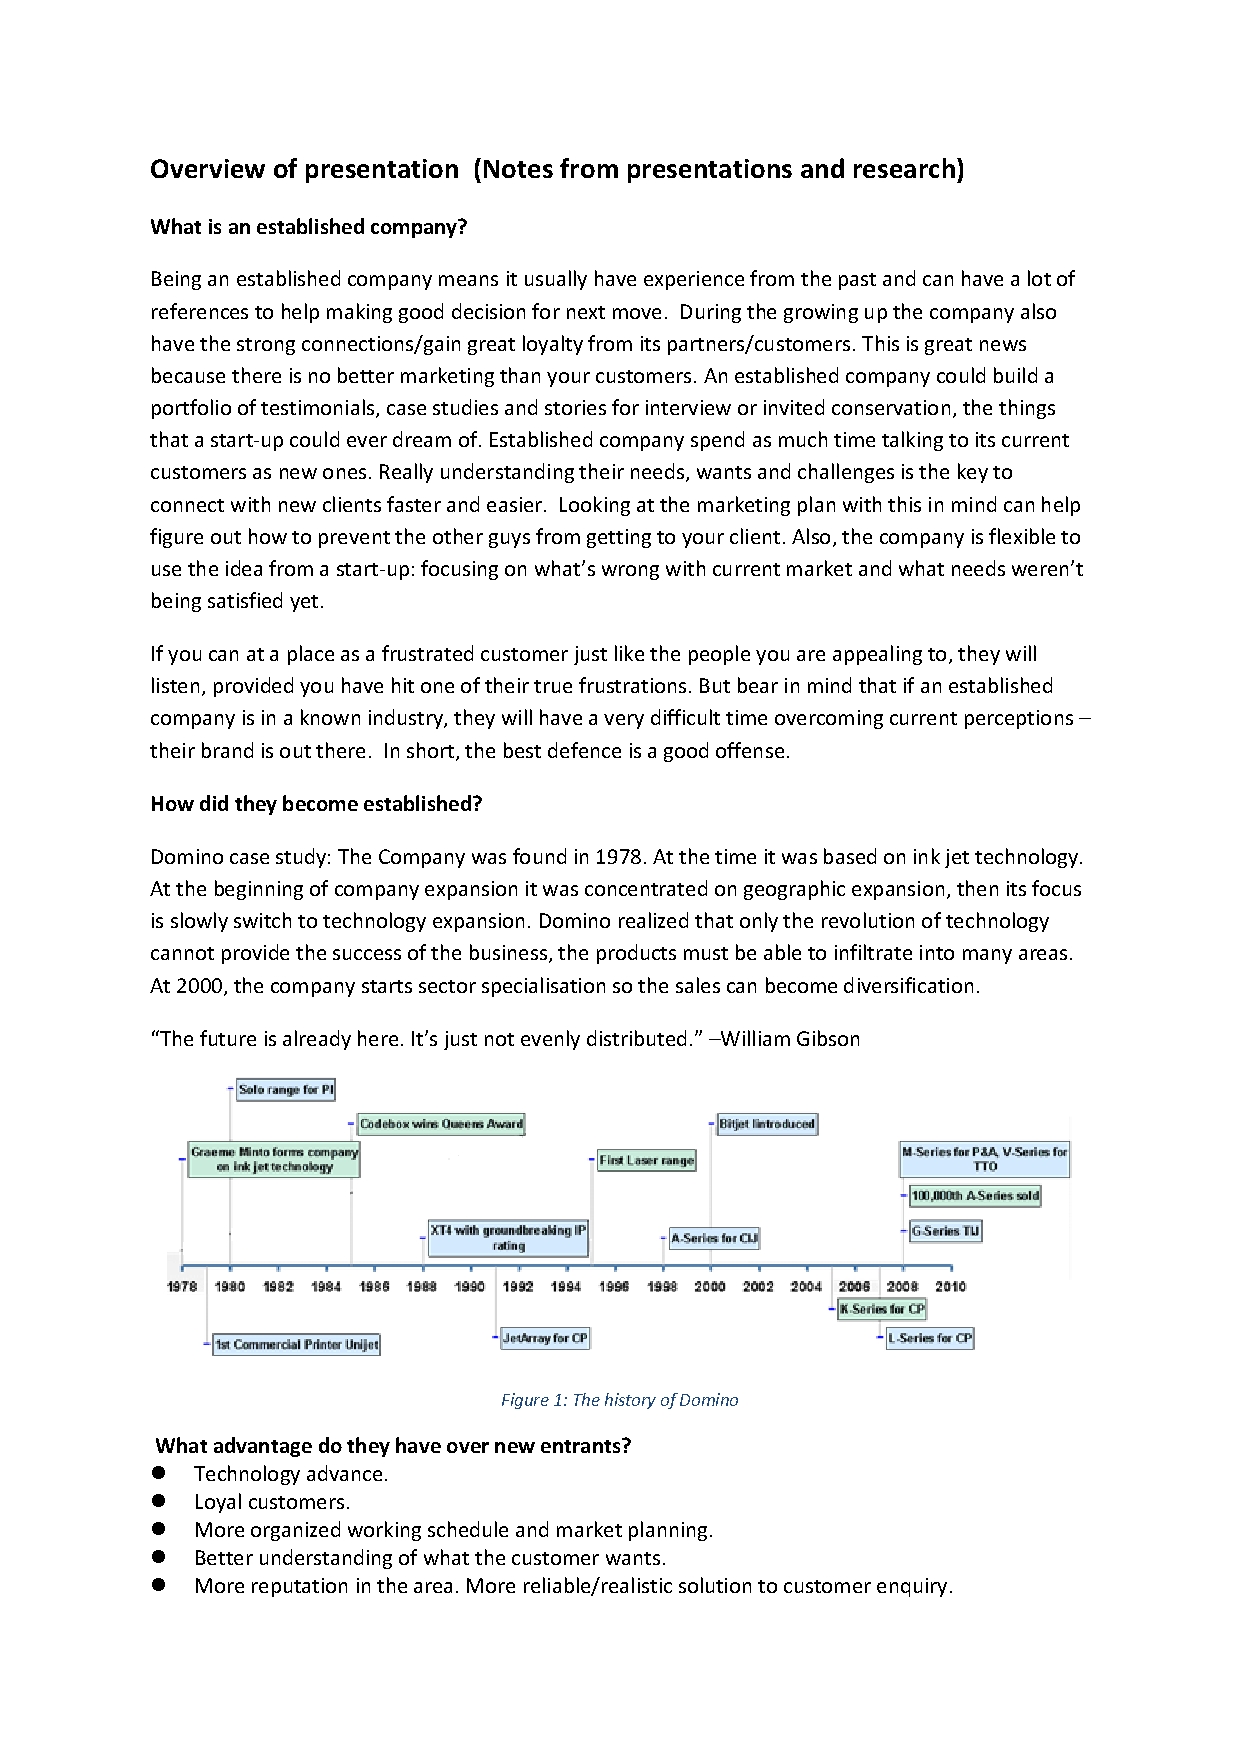
\includegraphics[width = 0.9\textwidth]{Figures/Overview_of_presentations}
		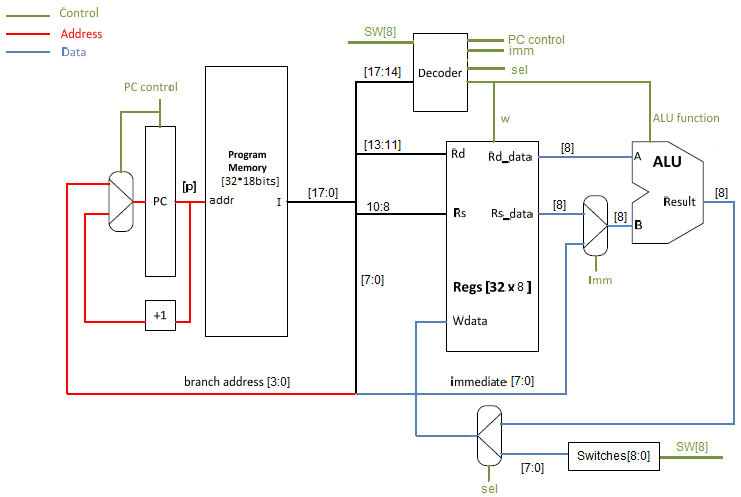
\includegraphics[width = 0.8\textwidth]{Figures/oldarch}		
		\caption{The origianl picoMIPS architecture design \cite{oldarcdigram}}
		\label {fig:oldarc}
\end{figure}
\begin{table}[H]

\centering % used for centering table
\begin{tabular}{c c c } % centered columns (4 columns)
\hline\hline %inserts double horizontal lines
Instruction                 & Acronym     & Description \\ [0.5ex] % inserts table
%heading
\hline % inserts single horizontal line
Addition                    & ADD         & \(Rd \leftarrow Rd + Rs \)  \\
Addition immediate          & ADDI        & \(Rd \leftarrow Rd + Imm\)      \\
Load switches SW[7:0]       & LOAD        & \(Rd \leftarrow Switches[7:0]\)      \\
Multiply immediate          & MUXI        & \(Rd \leftarrow Rd \times Imm\)      \\
Wait while SW[8]= 0         & WAIT0       & \(if(SW[8] = 1) PC++     \)          \\
Wait while SW[8]= 1         & WAIT1       & \(if(SW[8] = 0) PC++  \)         \\
Absolute jump               & JUMP        & \(PC \leftarrow 0  \)             \\ [1ex] % [1ex] adds vertical space
\hline %inserts single line
\end{tabular}
\caption{Instruction Set} % title of Table
\label{table:instr} % is used to refer this table in the text
\end{table}

\subsection{Control Instruction} \label{SubSection:Control Instruction}

The affine transform does not require any decisions based on the data. Therefore there is no flag needed, neither is the conditional branch. The only necessary control signal is for the handshaking procedure, and it comes from switch SW8. During the handshaking, the program counter will not increment until value of switch SW8 is correct. In this case, instruction \textit{WAIT0} and \textit{WAIT1} were implemented to accomplish this operation. At the end of the affine transform, an absolute jump is essential for returning the transform operation to the start. The instruction \textit{JUMP} replaces the value of the program counter with its last four bits. So in fact, it can make the processor to jump to any instruction location. But in this project, it only resets the program counter. 

\subsection{Arithmetic and register instruction} \label{SubSection:Arithmetic and register instruction}
In order to accomplish an affine transform, at least two kinds of arithmetic are needed: addition and multiplication. In the processor, the corresponding arithmetic instructions were \textit{ADD} and \textit{MUX}. They consist of the operand codes that will deliver operating commands to Arithmetic Logic Unit (ALU), designated source and destination register addresses. In addition, instruction \textit{ADDI} and \textit{MUXI} were developed for the arithmetic with signed immediate values. The immediate instructions select build-in immediate values rather than the ones from source register. It is very convenient when used in the calculations with matrix constants. No subtract instruction was implemented to reduce the size of the ALU.\\\\
At the beginning of the affine transform, x1 and y1 values are provided by the switches. The processor needs to read and store them in the certain memory locations. Therefore a store instruction \textit{LOAD} is implemented for this purpose. Since the register will also be accessed in conjunction with other arithmetic instructions, the register addresses are included in those instructions. 
	
\section{Program Counter, Program memory and Decoder design} 

\subsection{Program Counter} \label{Program Counter}
Program counter is the simplest sequential logic module in the system. The counter will increment every clock cycle if the increment control signal \textit{PCincr} is high. If the \textit{JUMP} instruction is called, the absolute branch control signal \textit{PCabsbranch} will force the counter to jump to the address given by the instruction. In this case, it would be the start position of the operation. The program counter size was set to 5 bits, so it can count up to 32 instructions. 

\lstset{language=verilog,caption={Testbench for program counter},label=pctest}
\begin{lstlisting}
module pctest;
 parameter Psize = 5;
 logic clk, reset, PCincr,PCabsbranch;
 logic [Psize-1:0] Branchaddr;
 logic [Psize-1 : 0]PCout;
 
pc  #(.Psize(Psize)) P(.*);

//------------- code starts here ---------
//clock
initial
begin
  clk =  0;
  #5ns  forever #5ns clk = ~clk;
end

initial
begin
  //default
 reset = 1;
 PCincr = 0;
 Branchaddr = 4'b0000; 
 PCabsbranch = 0;
  
  // test all functions
  #10 reset = 0; 
  #10 PCincr = 1; //start counting
  #10 PCincr = 0; //stop counting
  #10 PCincr = 1;
  #50 PCabsbranch = 1;PCincr = 0; //JUMP
  #10 PCabsbranch = 0;
  #10 PCincr = 1;

end

endmodule //end of pctest
\end{lstlisting}

\begin{figure}[ht!]
		\centering
		%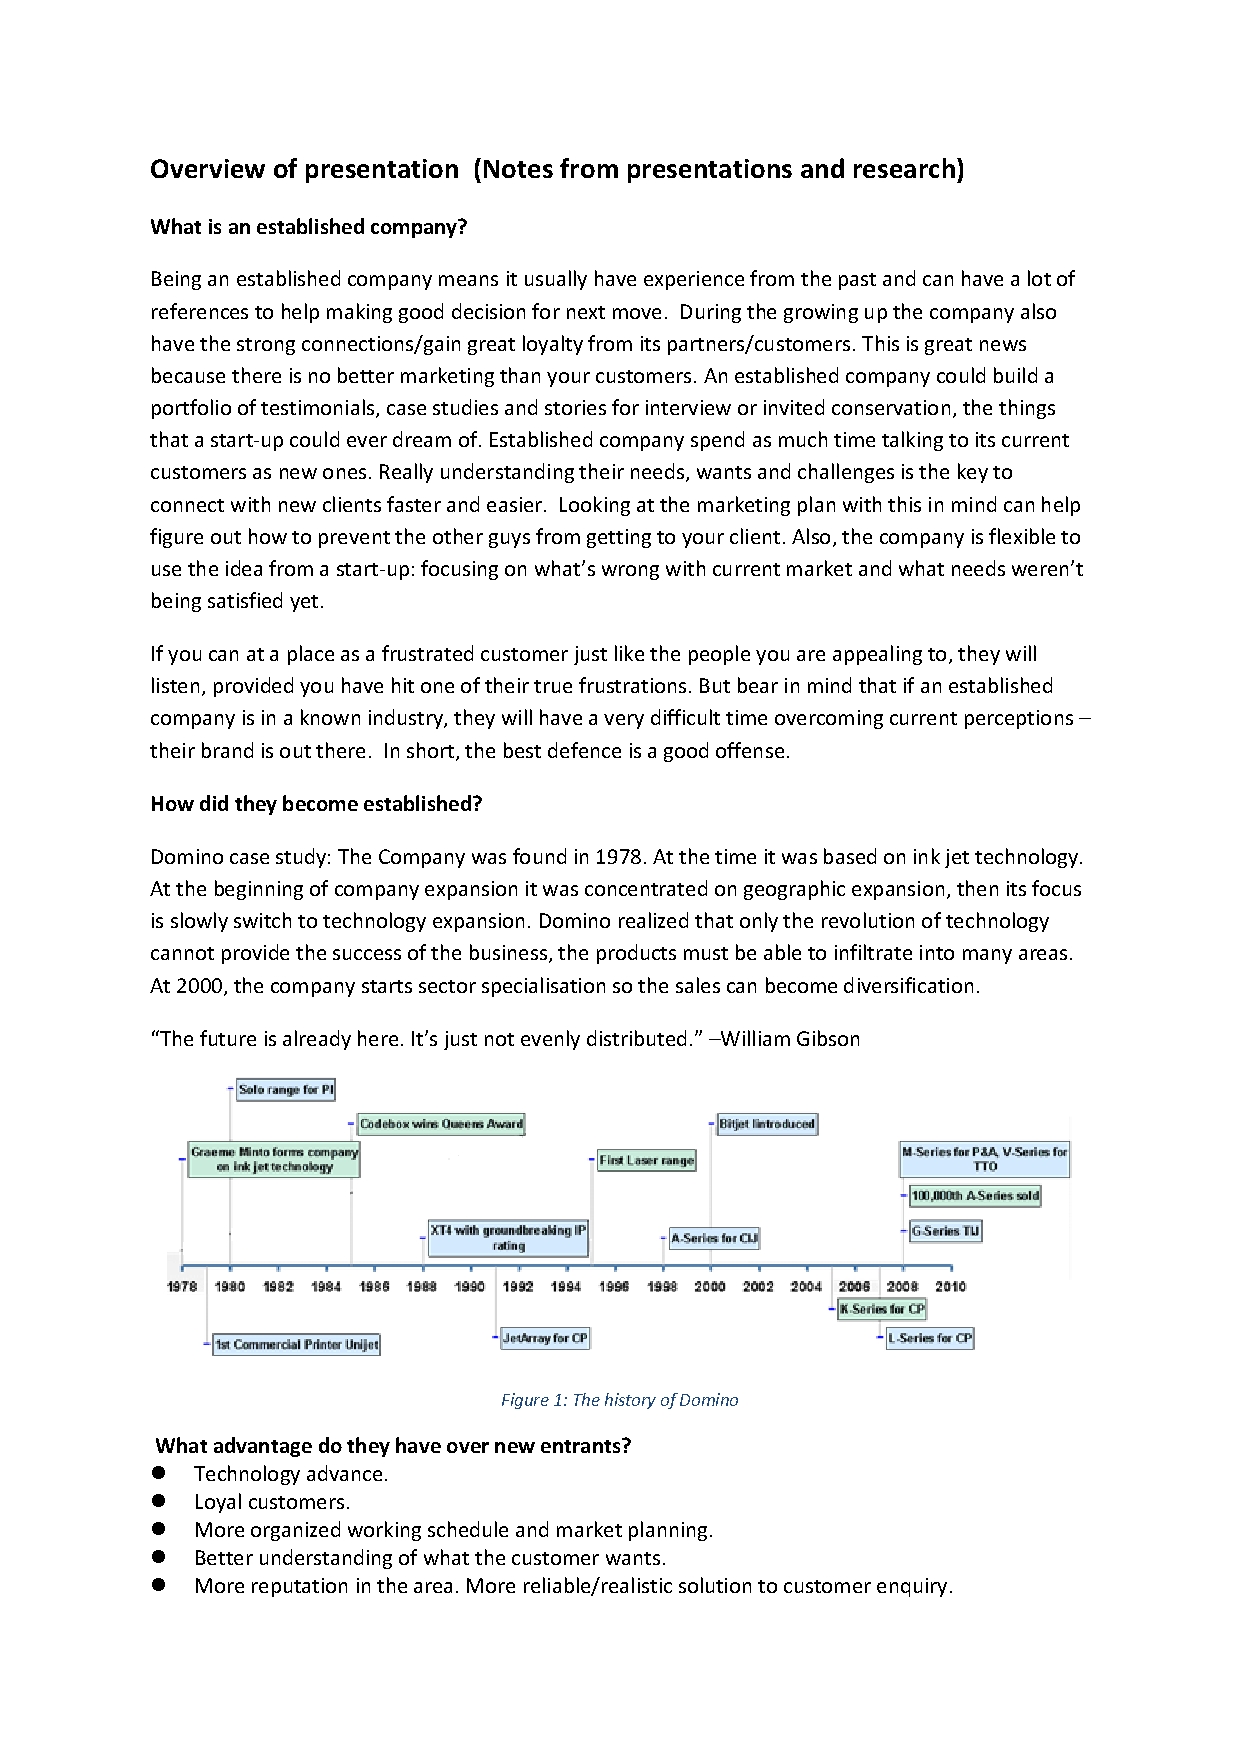
\includegraphics[width = 0.9\textwidth]{Figures/Overview_of_presentations}
		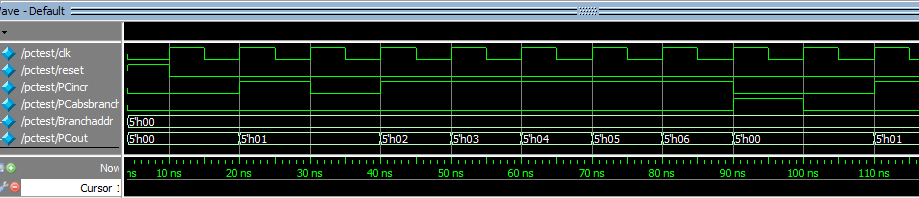
\includegraphics[width = \textwidth]{Figures/PC}		
		\caption[Additional Notes]{Testbench result of Program Counter}
		\label {fig:pc}
\end{figure}

The testbench and simulation result of program counter are shown in listing~\ref{pctest} and Figure~\ref{fig:pc}. At 20ns, the increment control signal PCincr went high so the counter started to count up. At 30ns, PCincr went low so counter stopped counting at the current clock cycle. At 90ns, the testbench simulated a \textit{JUMP} instruction: \textit{PCincr} became low and absoluate branch control signal \textit{PCabsbranch} went high. In this case, the counter loads the address from Branch address \textit{Brachaddr} (0000) and restarts the counting.\\\\
The RTL level synthesis of program counter is shown in Figure ~\ref{fig:counter}.

		\begin{figure}[ht!]
		\centering
		%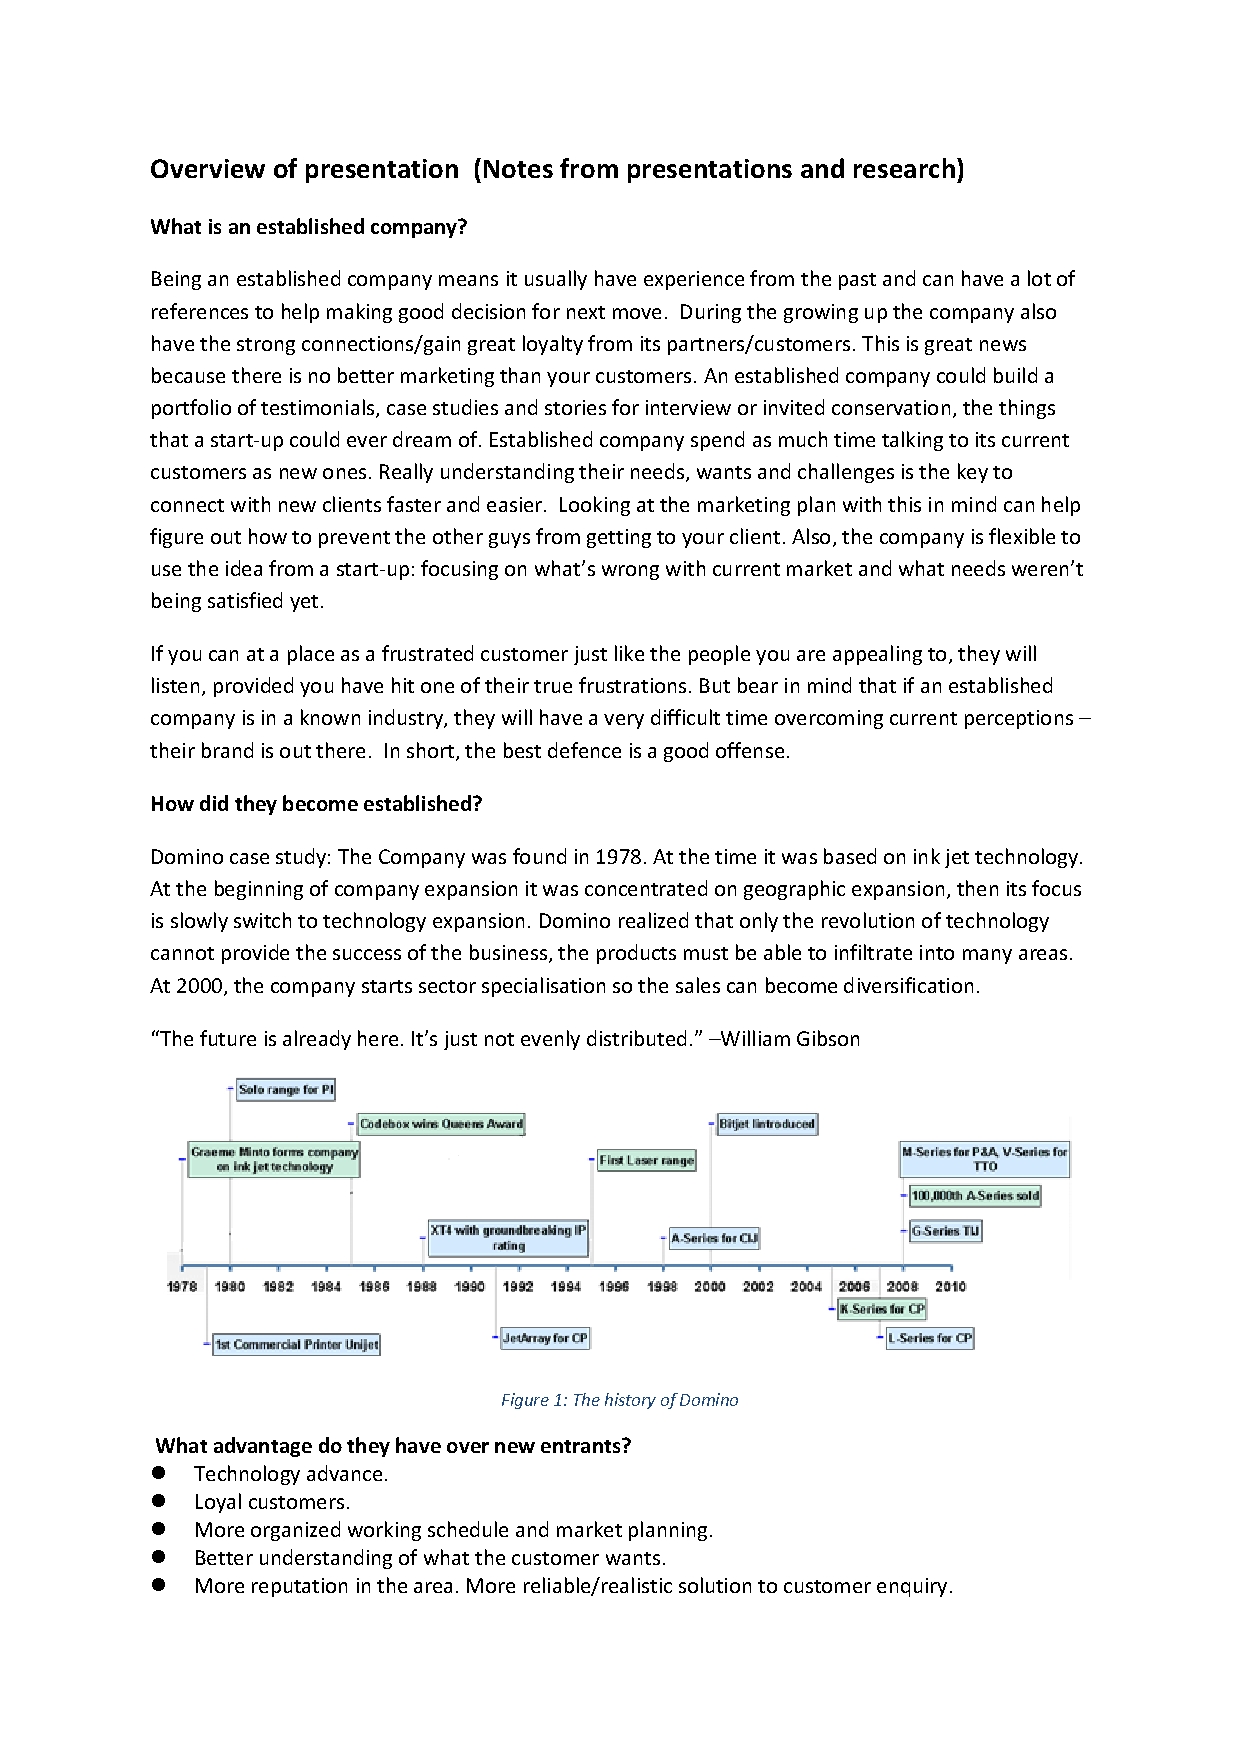
\includegraphics[width = 0.9\textwidth]{Figures/Overview_of_presentations}
		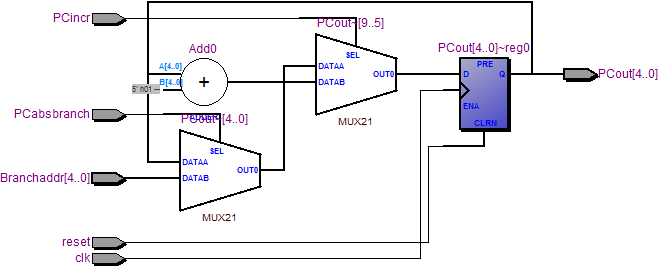
\includegraphics[width = \textwidth]{Figures/counter}		
		\caption{RTL synthesis of Program Counter}
		\label {fig:counter}
	\end{figure}

\subsection{Program Memory} \label{Program Memory}

In general, the program memory is a ROM with asynchronous read. It has one input port to receive the address sent by program counter. The address extracts the corresponding instruction stored in the memory to the output port. All the instructions were decoded in hexadecimal format and stored in the separate hex file \textit{prog.hex}. During the initiation of the program memory, this file was loaded into the program RAM. The program address width and instruction length were acquired for the declaration of the program memory.\\\\
The testbench codes are demonstrated in listing~\ref{pmtest}.

\lstset{language=verilog,caption={Testbench for program Memory},label=pmtest}
\begin{lstlisting}

module progtest;
parameter Psize = 5, Isize = 18;
logic [Psize-1:0] address;
logic [Isize-1:0] I; // I - instruction code

// program memory declaration, note: 1<<n is same as 2^n
logic [Isize:0] progMem[ (1<<Psize)-1:0];

prog #(.Psize(Psize),.Isize(Isize)) r(.*);

//------------- code starts here ---------
initial
begin
  //try all the memory address
  address [Psize-1:0] = 5'h00;
  #10ns  address [Psize-1:0] = 5'h01; 
  #10ns  address [Psize-1:0] = 5'h02;
  #10ns  address [Psize-1:0] = 5'h03;
  #10ns  address [Psize-1:0] = 5'h04;
  #10ns  address [Psize-1:0] = 5'h05;
  #10ns  address [Psize-1:0] = 5'h06;
  #10ns  address [Psize-1:0] = 5'h07;
  #10ns  address [Psize-1:0] = 5'h08;
  #10ns  address [Psize-1:0] = 5'h09;
  #10ns  address [Psize-1:0] = 5'h0A;
  #10ns  address [Psize-1:0] = 5'h0B;
  #10ns  address [Psize-1:0] = 5'h0C;
  #10ns  address [Psize-1:0] = 5'h0D;
  #10ns  address [Psize-1:0] = 5'h0E; 
  #10ns  address [Psize-1:0] = 5'h0F; 
  #10ns  address [Psize-1:0] = 5'h10; 
  #10ns  address [Psize-1:0] = 5'h11;
  #10ns  address [Psize-1:0] = 5'h12;              
end

endmodule // module regstest
\end{lstlisting}

\begin{figure}[H]
		\centering
		%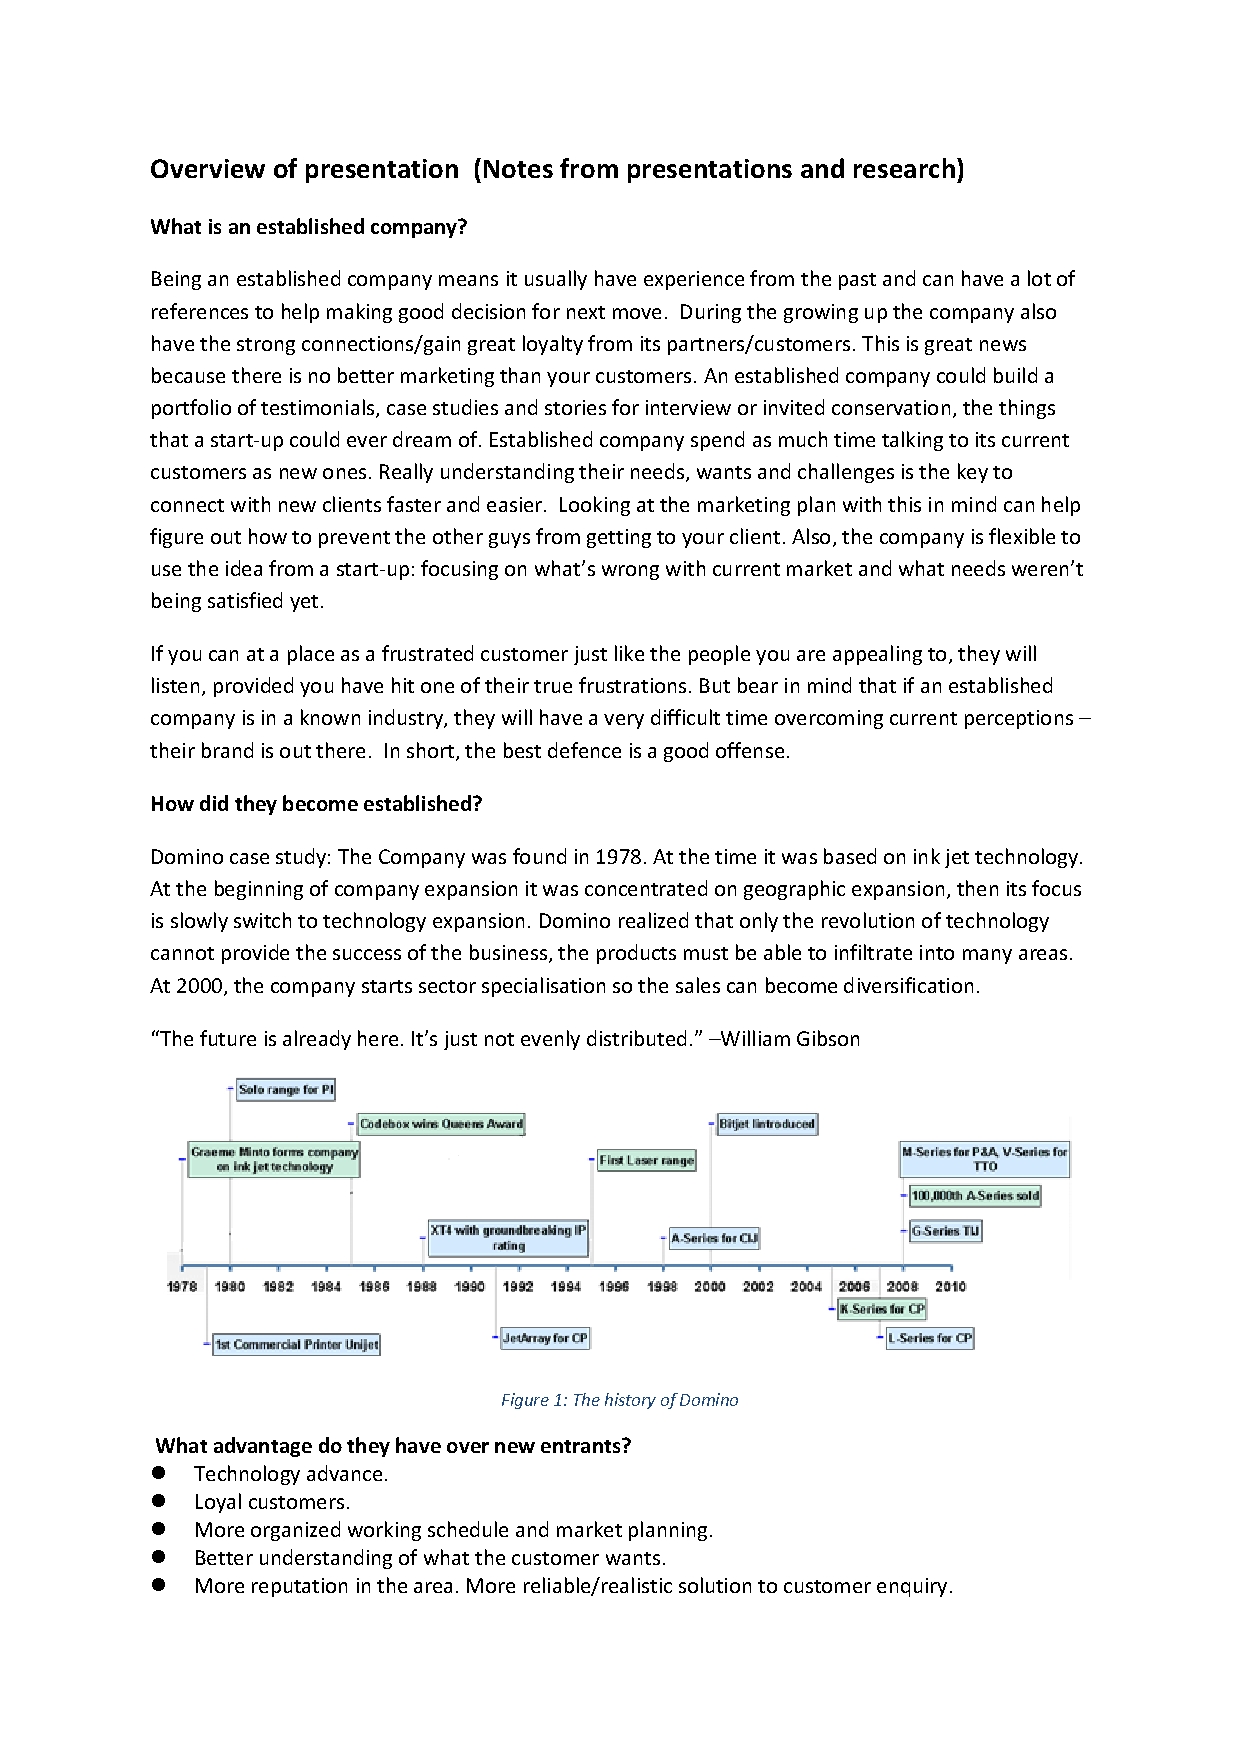
\includegraphics[width = 0.9\textwidth]{Figures/Overview_of_presentations}
		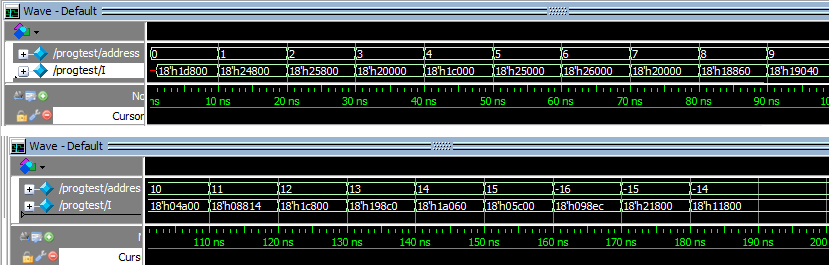
\includegraphics[width = \textwidth]{Figures/PM}		
		\caption[Additional Notes]{Testbench result of Program Memory}
		\label {fig:pm}
\end{figure}

As shown in Figure~\ref{fig:pm}, when the testbench feed an address to the program memory, the corresponding instruction was extracted at the output. The testbench attempted all the memory address and outputted instructions were verified correct according to the hex file \textit{prog.hex}. \\\\
The RTL synthesis of program memory is shown in Figure~\ref{fig:memory}. Note that the write-enable of the memory is always zero, which makes the program memory a READ-ONLY memory.
		\begin{figure}[H]
		\centering
		%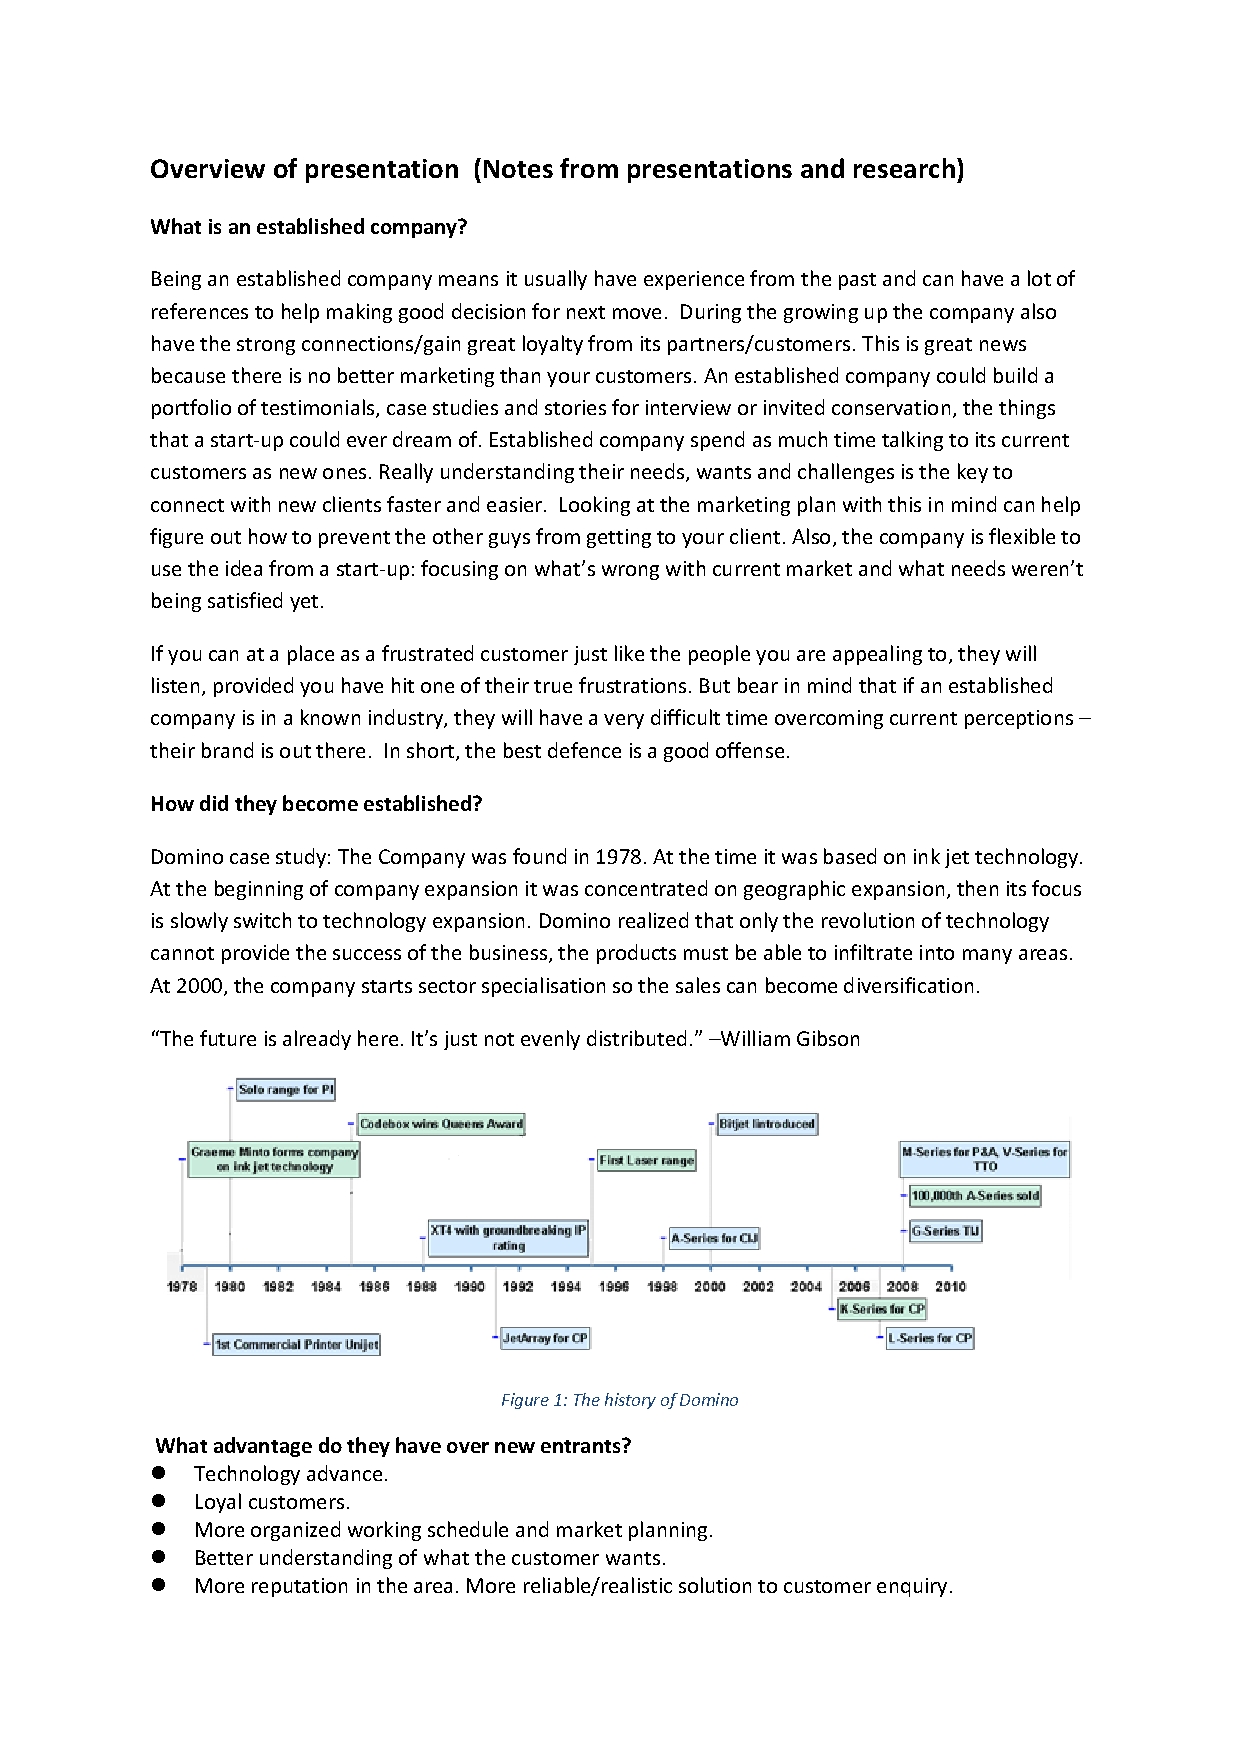
\includegraphics[width = 0.9\textwidth]{Figures/Overview_of_presentations}
		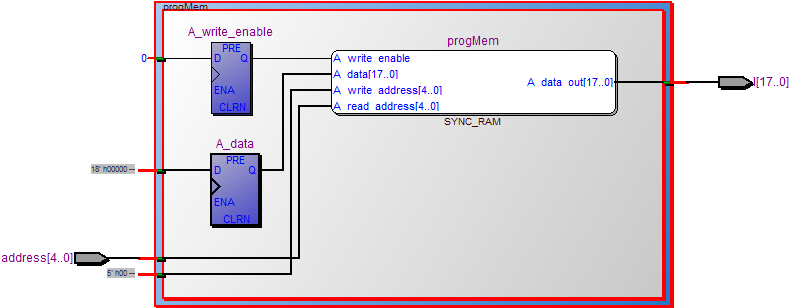
\includegraphics[width = \textwidth]{Figures/progmem}		
		\caption{RTL synthesis of Program Memory}
		\label {fig:memory}
	\end{figure}

\subsection{Decoder} \label{Decoder}
The decoder was implemented as a combinational logic. It decodes the opcodes, which is the first four bits of the instruction. Eight types of instructions mentioned in the instruction chapter will be read from the program memory and translate into the control signals for ALU, program counter and general purpose register. The decoder also reads the control signal from switch SW[8] on the top level so the instruction \textit{WAIT0} and \textit{WAIT1} can be executed correctly. If an unexpected opcode is provided in the decoder, an error message will display for the debugging. Each opcode was defined in file \textit{opcodes.sv}. So it is easier to recognize and edit during the programming. ALU function control signals were defined in file \textit{alucodes.sv} for the same purpose. This file is also used in Arithmetic Logic Unit (ALU).\\\\ 
The opcode part of the decoder code is show in the listing~\ref{decoder}. 
\lstset{language=verilog,caption={Opcode part of Decoder code},label=decoder}
\begin{lstlisting}

module decoder;
.....
 case(opcode)
     //do nothing
     `NOP: PCincr = 1'b1;
		
     //register-register add		
      `ADD:begin
	        w = 1'b1; // write result to dest register
	        PCincr = 1'b1;
	        ALUfunc = `RADD;
	      end
			
		 //register-immediate add
	     `ADDI:begin
	         w = 1'b1; 
			     imm = 1'b1; // select immediate operand
			     PCincr = 1'b1;
			     ALUfunc = `RADD;
		    end	 		
				
     //register-register multiply
	 	   `MUX: begin 
	         w = 1'b1; // write result to dest register
	         ALUfunc = `RMUX;
	         PCincr = 1'b1;
	      end	
		 
		 //register-immediate multiply		
	     `MUXI: begin 
	          w = 1'b1; 
	          imm = 1'b1;
	          ALUfunc = `RMUX;
	          PCincr = 1'b1;
	      end	 
				
		 //wait while 1			
	     `WAIT1: begin 
	         if(SW == 1'b1) //if SW[8] == 0 PC++
	          begin
	          PCincr = 1'b0;
	          sel = 1'b0;
	         end
	         else
	          begin
	          PCincr = 1'b1;	     
	          sel = 1'b0;
	         end
	      end
				
		 //wait while 0		
	     `WAIT0: begin   
	         if(SW == 1'b1) //if SW[8] == 1 PC++
	          begin
	          PCincr = 1'b1;
	          sel = 1'b0;
	          end
	         else
	          begin
	          PCincr = 1'b0;
	          sel = 1'b0;	
	          end     
	      end
				
 	   //Read Switches[7:0] and load into register
	     `LOAD: begin
	         w = 1'b1;
	         PCincr = 1'b1;
	         sel = 1'b1;
	     end 
			
     //JUMP (unconditional absolute branch)
	     `J:  begin
	         PCincr = 1'b0; 
					 PCabsbranch = 1'b1;
	     end
	      
	   default:
	   error("unimplemented opcode"); 
  endcase // opcode	
endmodule

\end{lstlisting}

Decoder Opcode is shown in listing ~\ref{opcode}.
\lstset{language=verilog,caption={opcode.sv},label=opcode}
\begin{lstlisting}
`define NOP   4'b0000
`define ADD   4'b0001
`define ADDI  4'b0010
`define J     4'b0100
`define MUX   4'b0101
`define MUXI  4'b0110
`define WAIT0 4'b0111
`define WAIT1 4'b1000
`define LOAD  4'b1001
\end{lstlisting}

Similar to program memory, the testbench examines all control signals can be decoded correctly for all types of opcode, as shown in listing~\ref{DCtest} .

\lstset{language=verilog,caption={Decoder testbench},label=DCtest}
\begin{lstlisting}
`include "alucodes.sv"
`include "opcodes.sv"

module decodertest;

logic [3:0] opcode; // top 6 bits of instruction
logic [2:0] ALUfunc;
logic SW;
logic PCincr,imm,w,PCabsbranch,sel;

decoder c(.*);
//------------- code starts here ---------

initial 
begin
  SW = 0;	
  #10ns opcode =4'b0111; //WAIT0
  #10ns SW=1; 
  #10ns opcode =4'b1000; //WAIT1
  #10ns SW=0;
  #10ns opcode =4'b1001; //LOAD
  #10ns opcode =4'b0110; //MUXI
  #10ns opcode =4'b0001; //ADD
  #10ns opcode =4'b0010; //ADDI
  #10ns opcode =4'b0100; //JUMP
  end
endmodule 
\end{lstlisting}

\begin{figure}[H]
		\centering
		%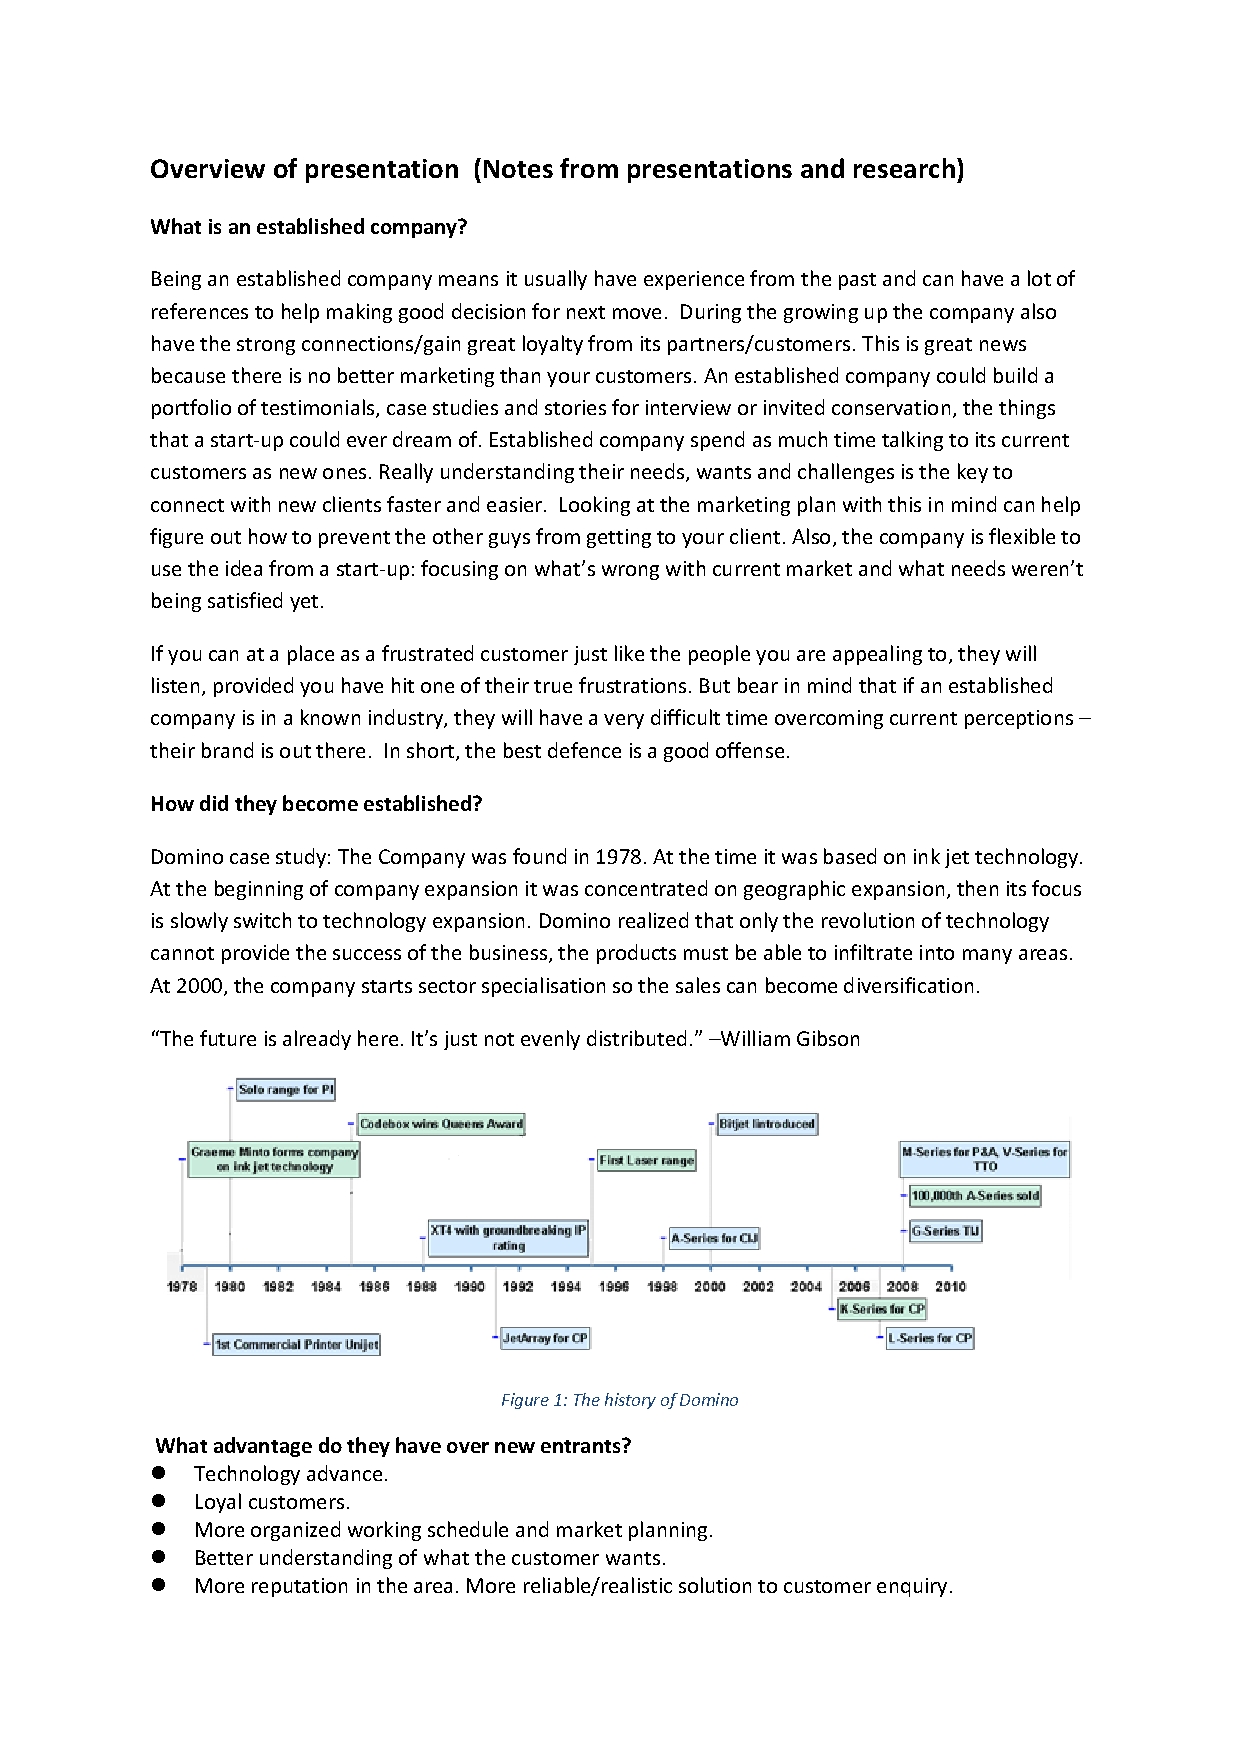
\includegraphics[width = 0.9\textwidth]{Figures/Overview_of_presentations}
		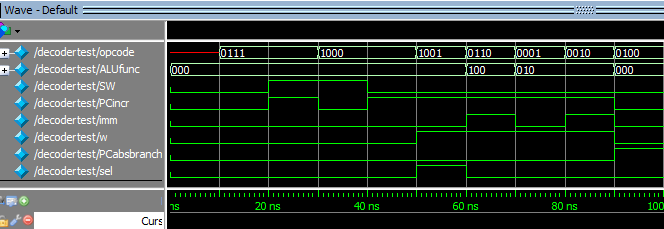
\includegraphics[width = \textwidth]{Figures/DC}		
		\caption{Simulation results of Decoder}
		\label {fig:DCtest}
\end{figure}

From the simulation results in Figure~\ref{fig:DCtest}, at 0ns, the program counter does not increment (PCincr = 0) in default state (no opcode input). When the opcode is \textit{ WAIT0} (at 10ns) or \textit{WAIT1} (at 30ns), the program counter signal \textit{PCincr} depends on switch signal \textit{SW}. \\\\
At 50ns, because the opcode is \textit{LOAD}, the "write-to-register" signal \textit{w} and "read-from-switches" signal \textit{sel} rise to high. The arithmetic opcode decoding test starts from 60ns. The decoder outputs the ALU control signal \textit{ALUfunc} accordingly, along with the write signal \textit{w}. If the arithmetic opcodes involve the immediate value (at 60ns and 80ns, the control signal \textit{imm} will rise to high. The last opcode in the simulation is \textit{JUMP}, therefore the absolute branch signal \textit{PCabsbranch} becomes high.\\\\
The RTL synthesis is shown in Figure~\ref{fig:decoder}.

\begin{figure}[H]
		\centering
		%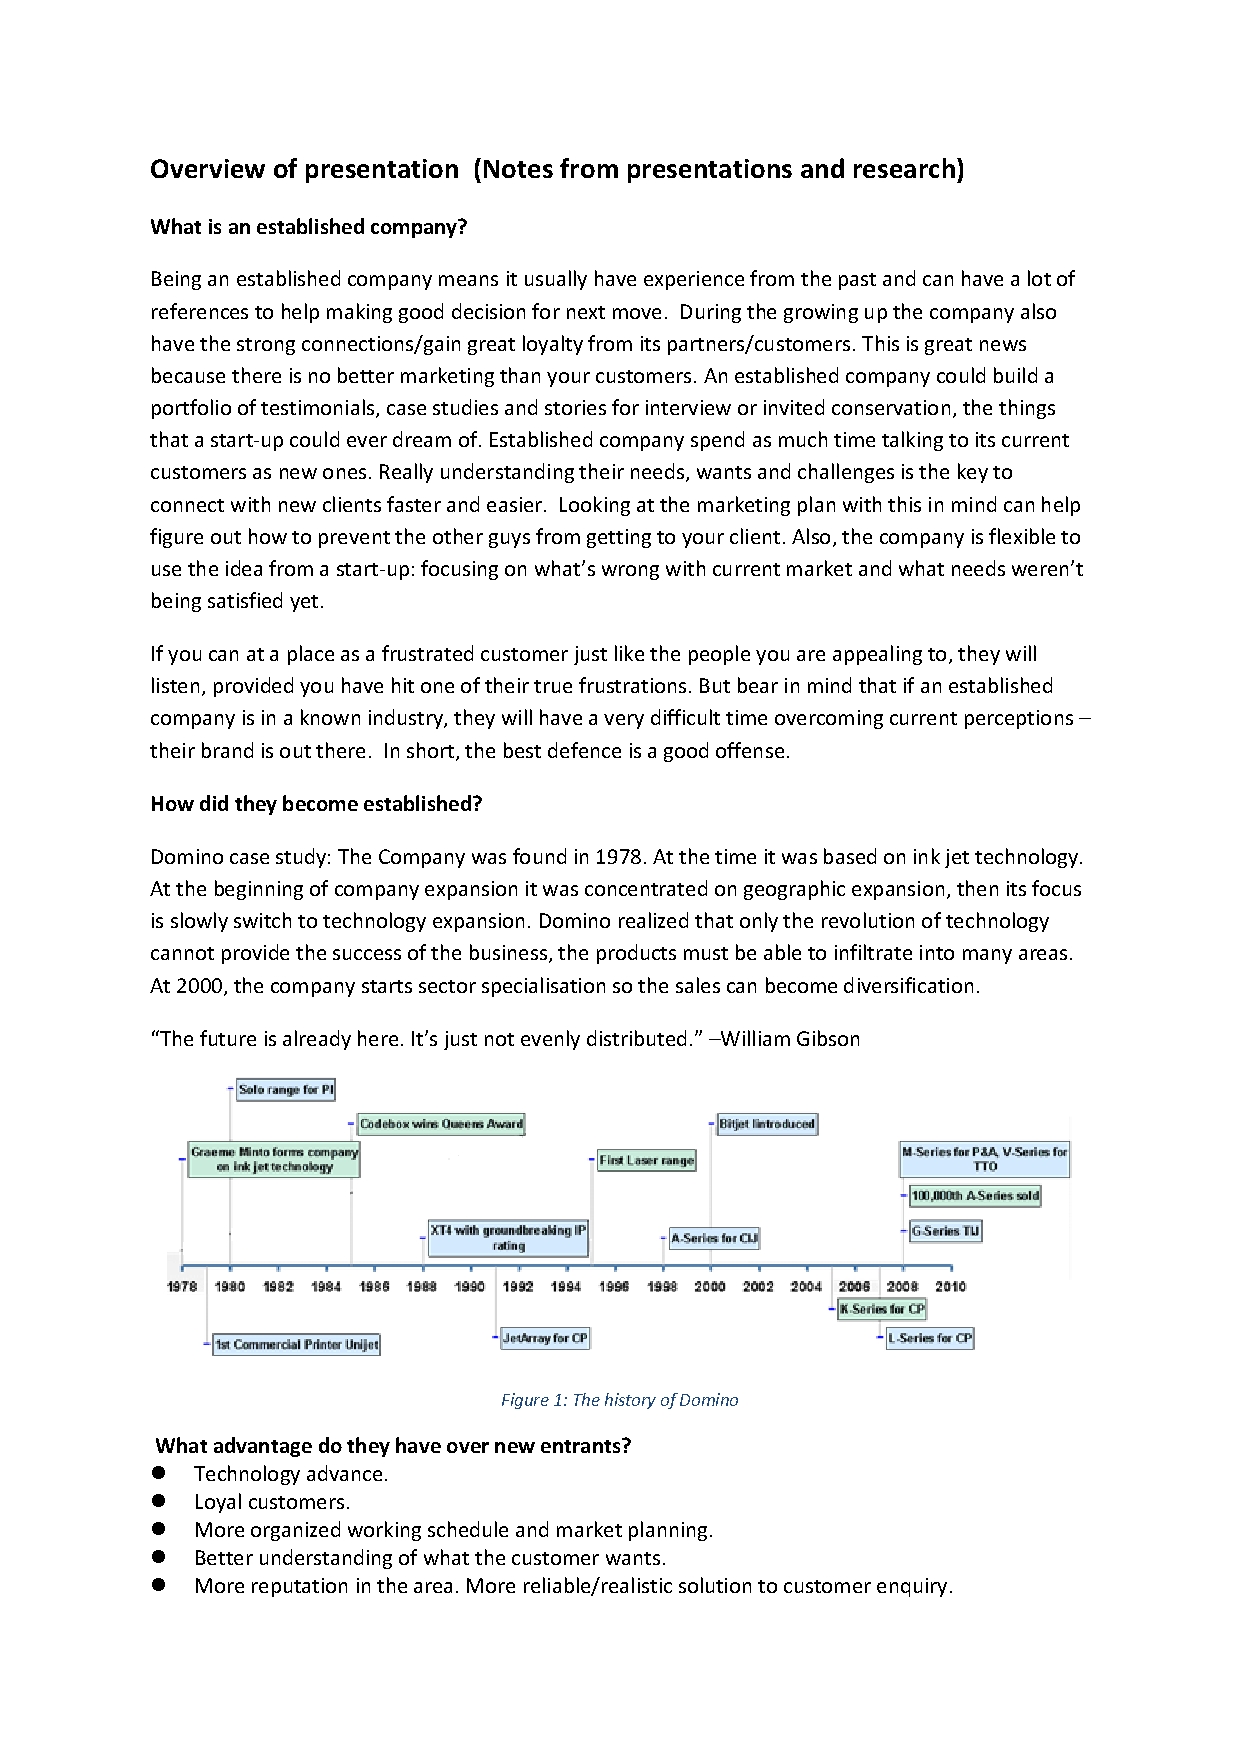
\includegraphics[width = 0.9\textwidth]{Figures/Overview_of_presentations}
		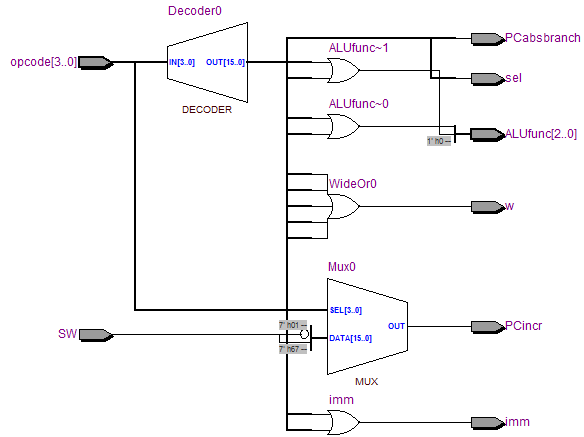
\includegraphics[width = 0.7\textwidth]{Figures/decoder}		
		\caption{RTL synthesis of Decoder}
		\label {fig:decoder}
\end{figure}

\section{General Purpose Register file design} \label{General Purpose Register}

The general purpose register was implemented as the multiple-port RAM with asynchronous read. It has two register address input ports and two register value output ports. The register-to-register calculation is greatly benefited of the dual-port design. In total there were five registers declared and each register could store one 8bits data. Different from the program memory, the general purpose register must also be able to restore the data to the designated address. However the register will not record the data only if the “write-to-register” signal \textit{w} from the decoder rises to high. The fifth to seventh bits of the instruction were used as the destination register address. Eighth and tenth bits were the source register address.\\\\
The testbench code is shown in listing~\ref{GDR}.
\lstset{language=verilog,caption={General Purpose Register testbench},label=GDR}
\begin{lstlisting}
module regstest;

parameter n = 8;
logic clk, w,reset;
logic [n-1:0] Wdata;
logic [2:0] Rdno, Rsno;
logic [n-1:0] Rd, Rs;

regs  #(.n(n)) r(.*);

//------------- code starts here ---------
//clock
initial
begin
  clk =  0;
  #5ns  forever #5ns clk = ~clk;
end

initial
begin
    w = 0;
    Wdata = 8'b00000000;
    reset = 1;
		Rdno = 0; Rsno =0;
  #10ns Wdata = 8'b00011111; reset =0;
  #10ns w =1; Rdno = 3'b001; //write data in register 1
  #10ns w = 0;
  #10ns Wdata = 8'b00001111;
  #10ns w =1; Rdno = 3'b010; //write data in register 2
  #10ns w=0;
  #10ns Rdno = 3'b001;//test Rd
  #10ns Rsno = 3'b010;//test Rs
end
endmodule // module regstest
\end{lstlisting}

\begin{figure}[H]
		\centering
		%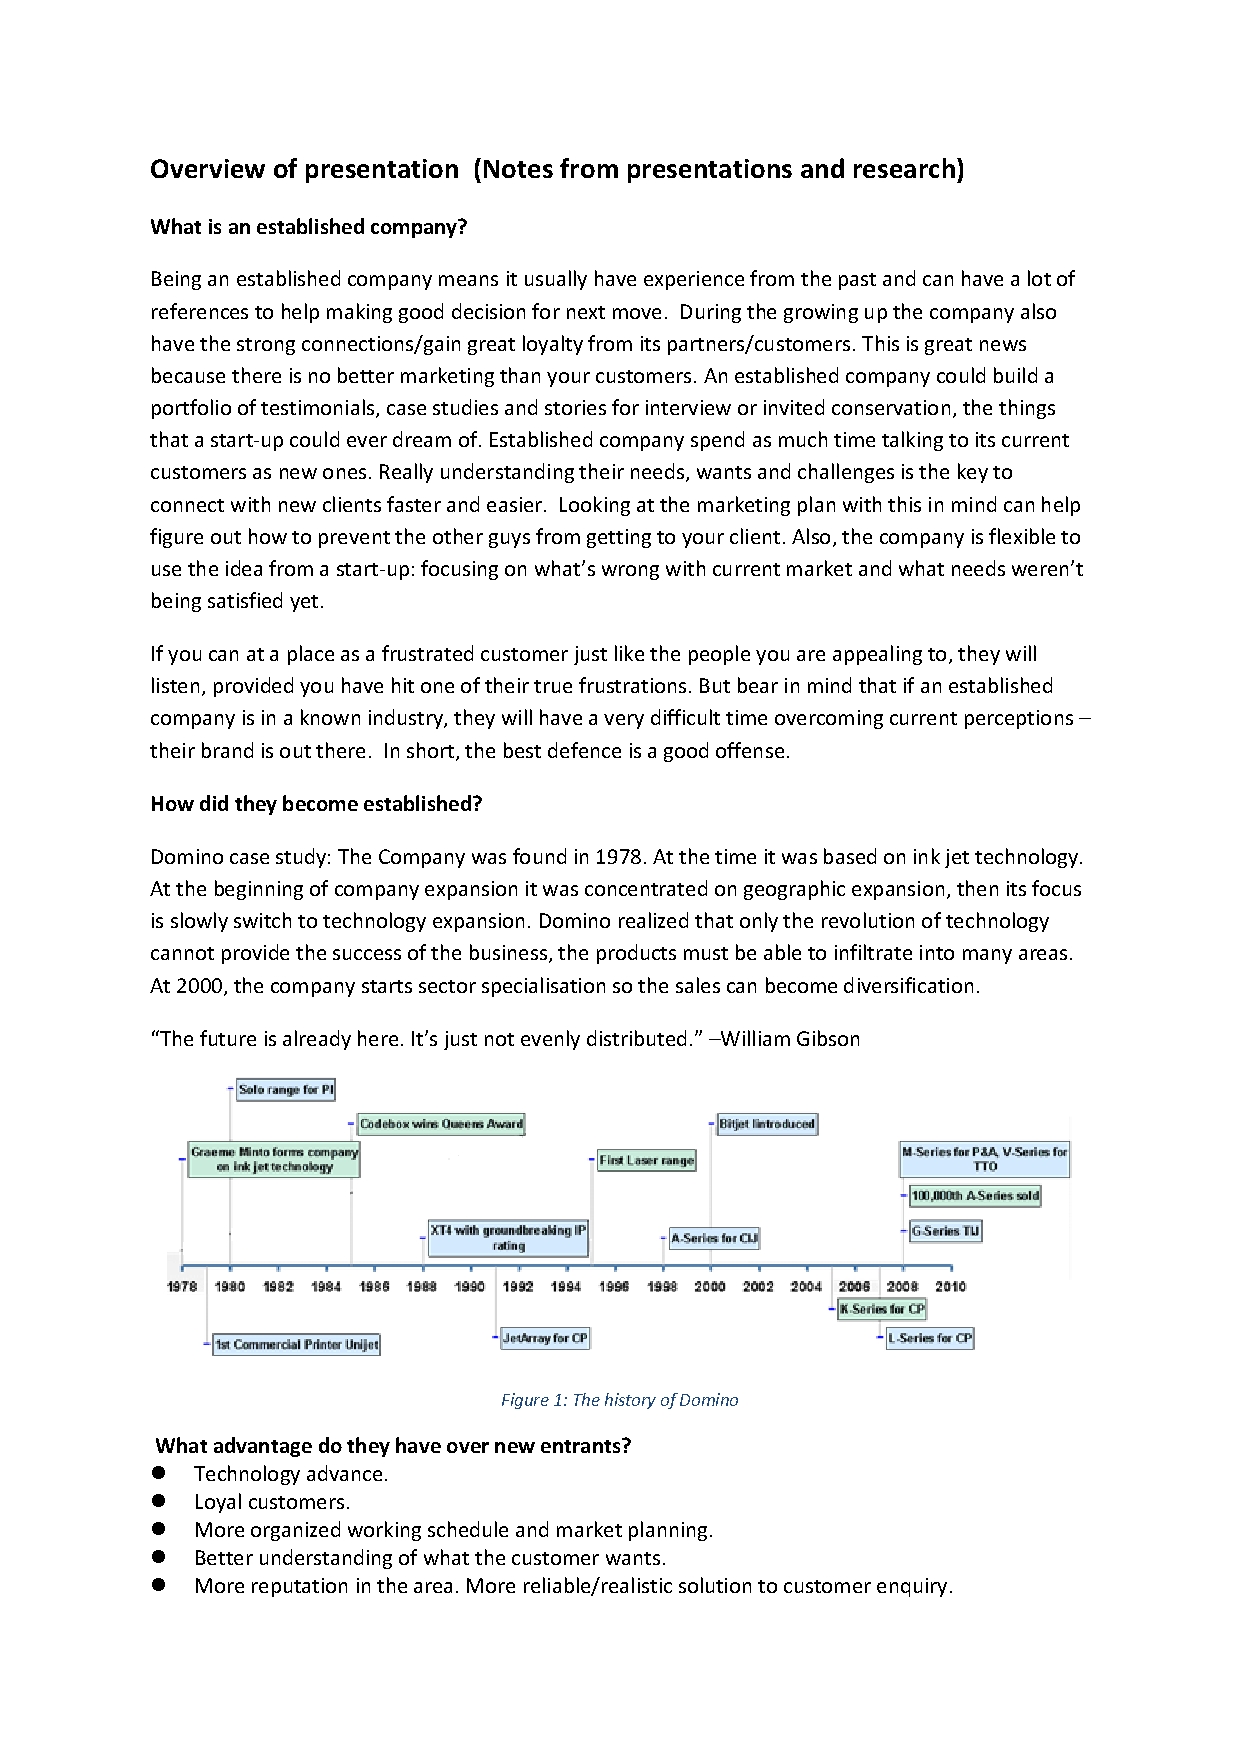
\includegraphics[width = 0.9\textwidth]{Figures/Overview_of_presentations}
		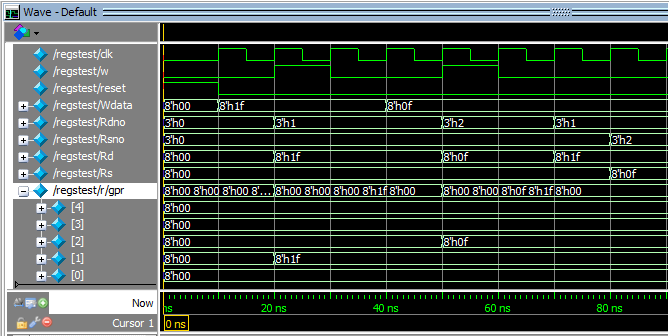
\includegraphics[width = \textwidth]{Figures/GPR}		
		\caption{Simulation results of General Purpose Register}
		\label {fig:GPRtest}
\end{figure}

In the testbench simulation there were two data written in the register 1 and 2 at different time. Because the register has asynchronous read, so the data could be written in and read out during the same clock cycle. At 70ns and 80ns, destination and source addresses were changed, and so were the data output at the destination and source register. This behaviour indicates the correct operation of the general purpose register. \\\\
However, Altera Cyclone III in FPGA only supports the synchronous memory block. Therefore the RTL synthesis tool have to use plenty of combinational logic units instead of the build-in RAM to create the required register. This results in a large size sequential register with no use of any memory bits, as shown in Figure~\ref{fig:register}.
\begin{figure}[H]
		\centering
		%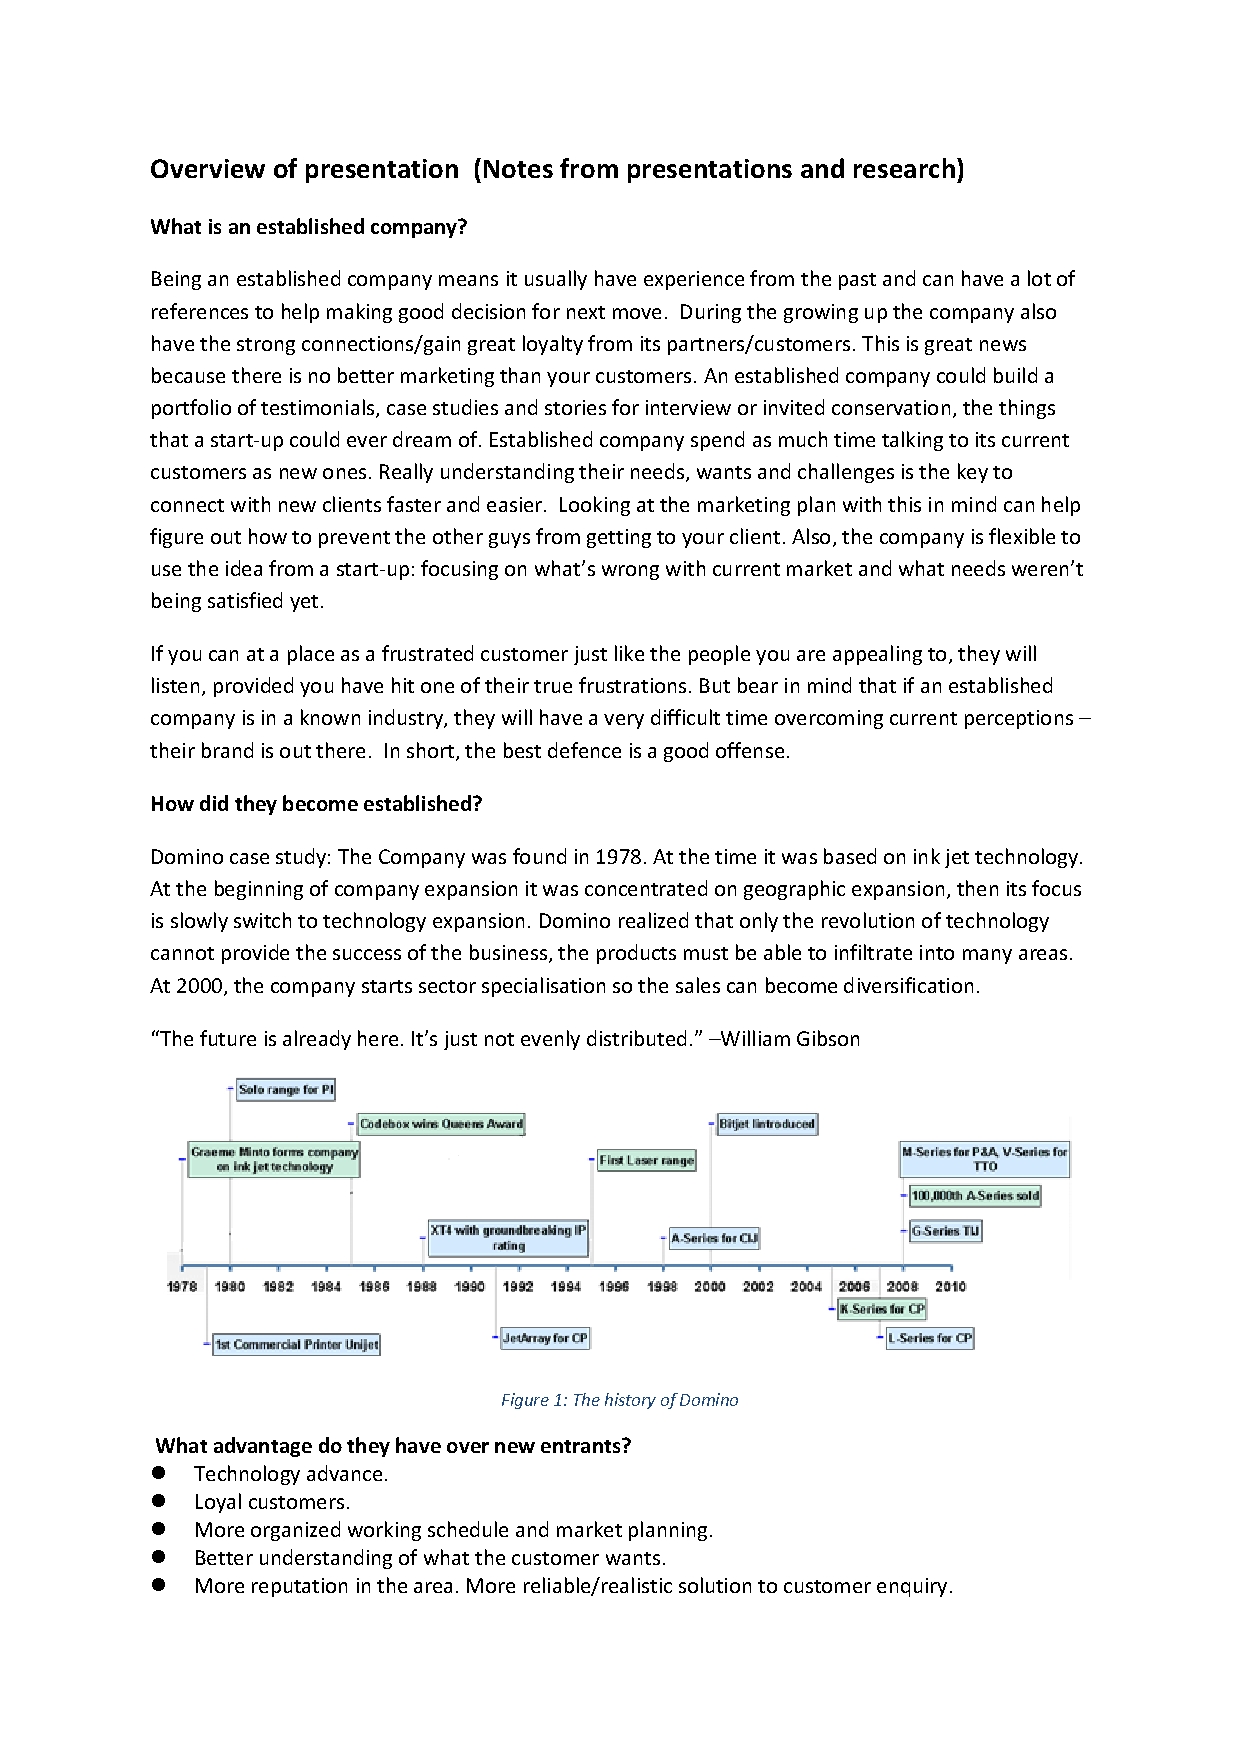
\includegraphics[width = 0.9\textwidth]{Figures/Overview_of_presentations}
		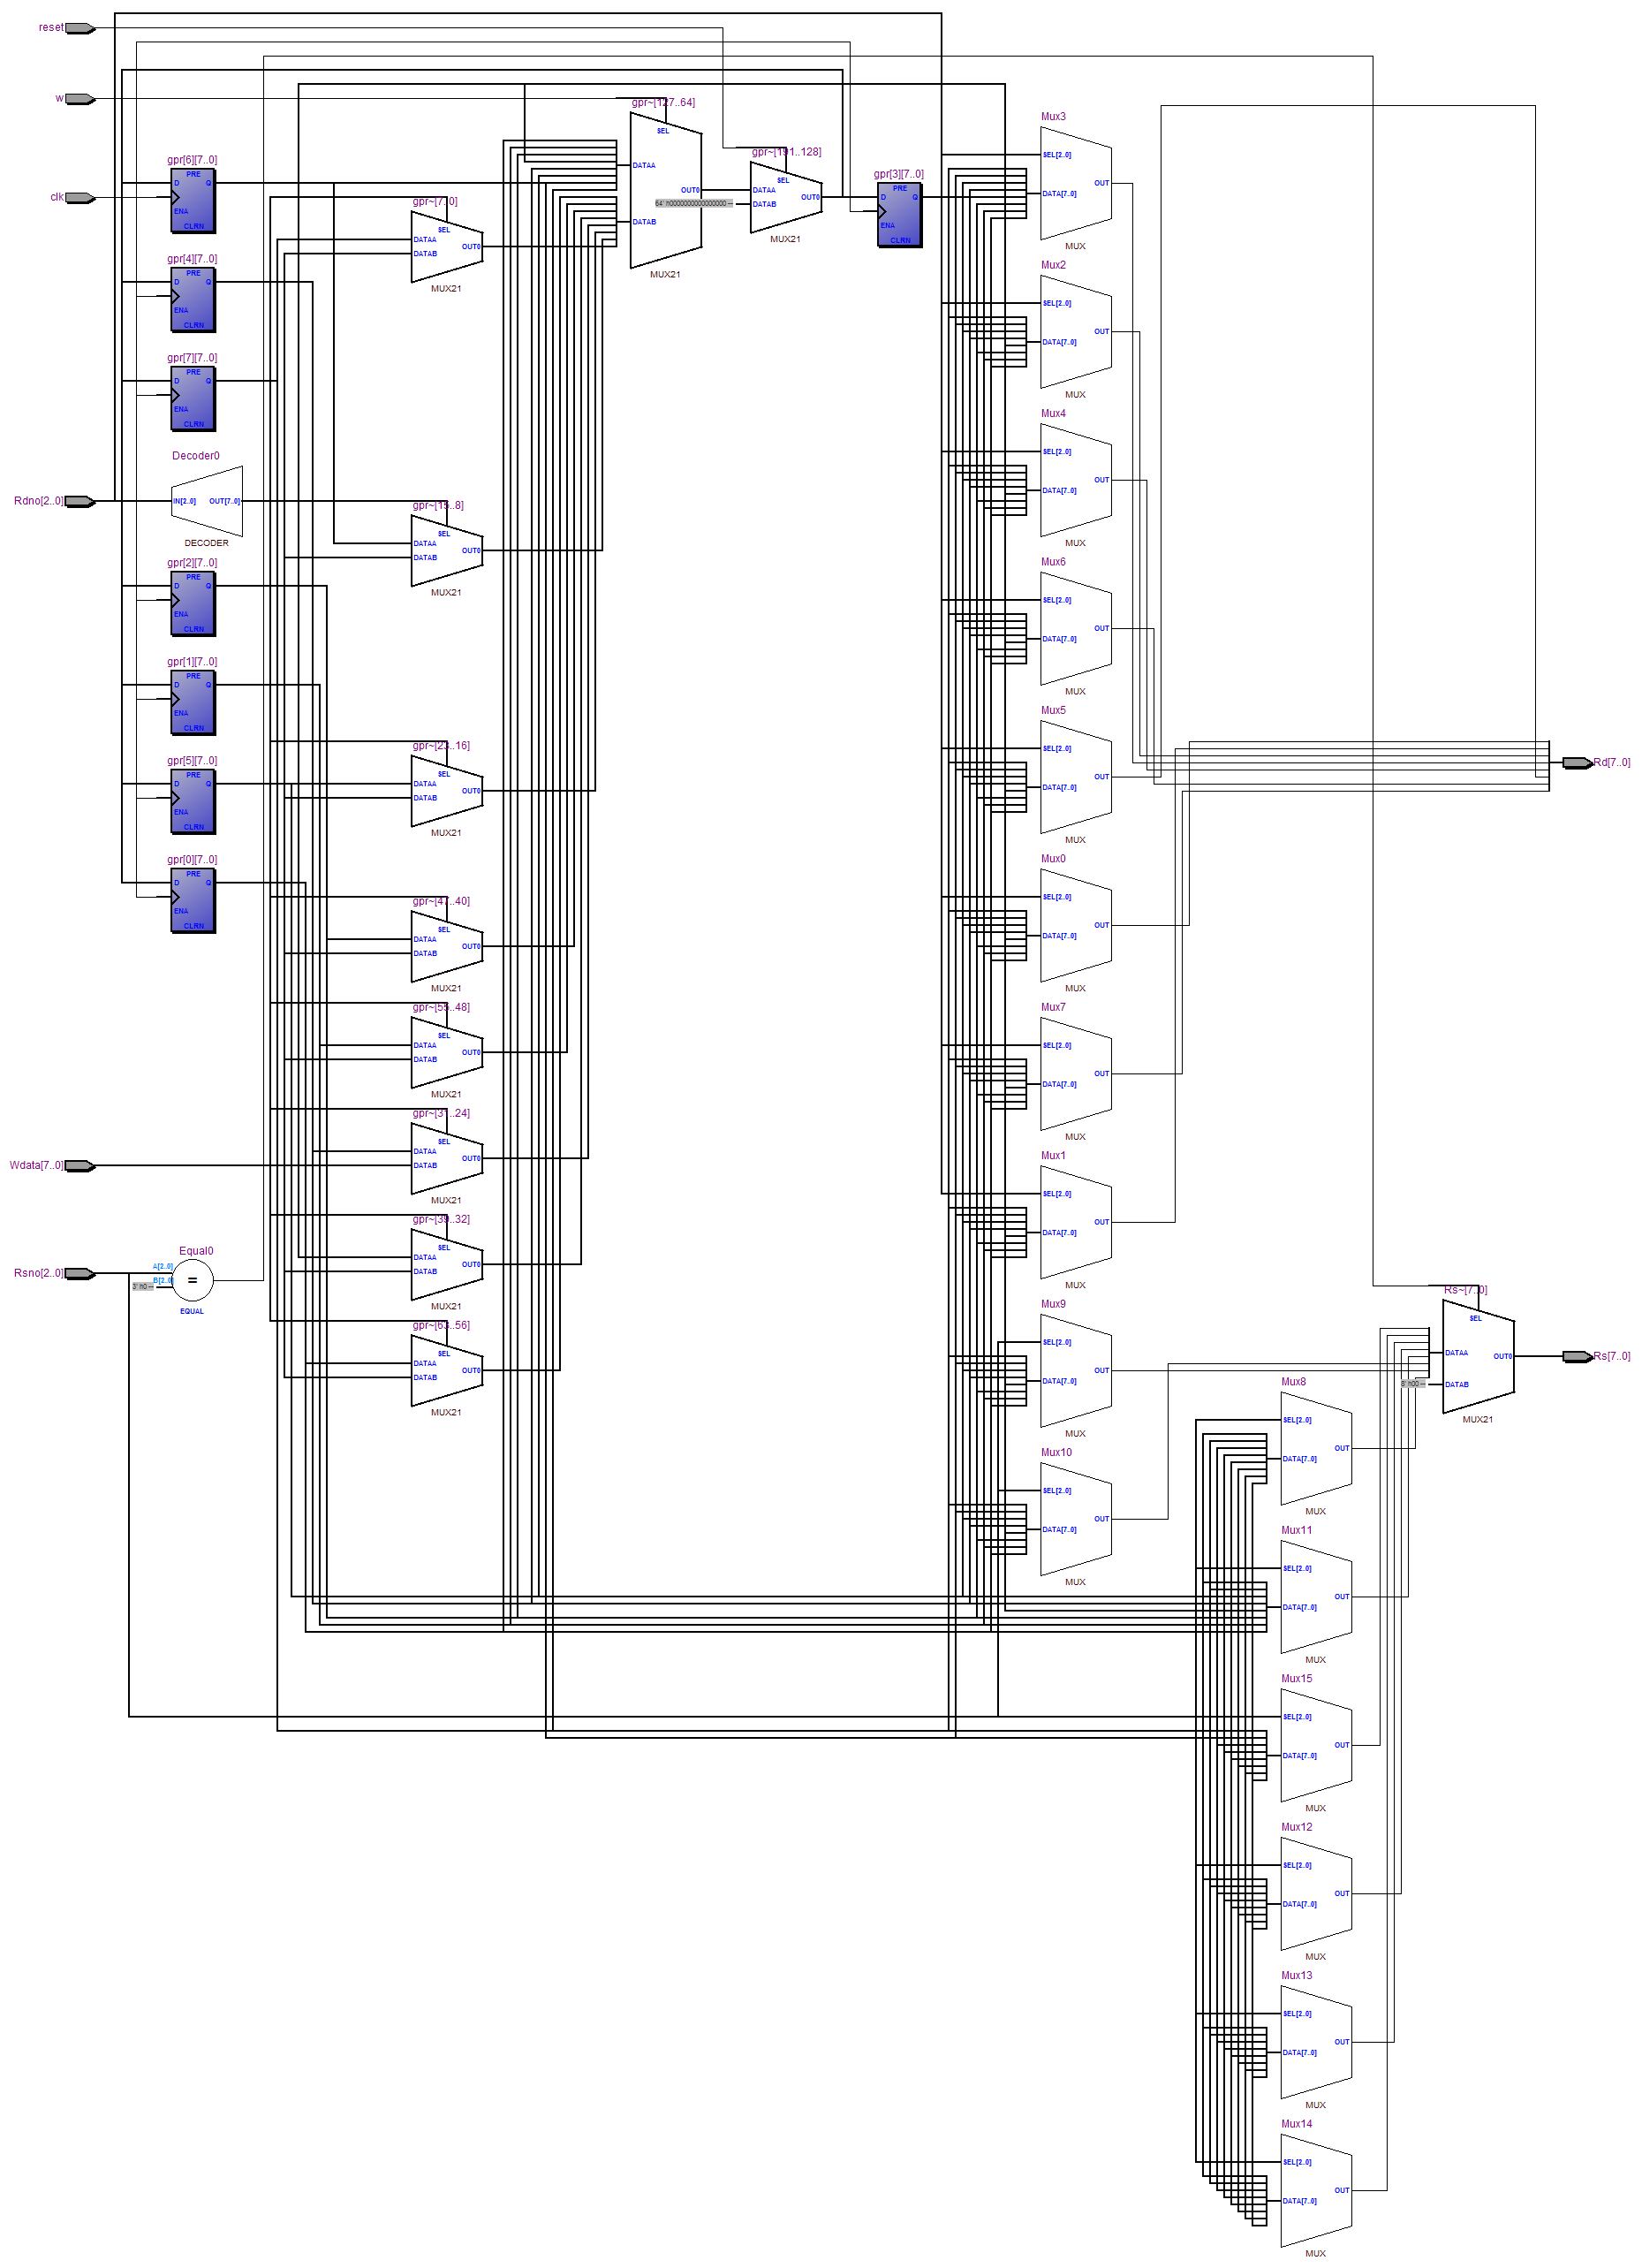
\includegraphics[width = \textwidth]{Figures/regs}		
		\caption{RTL synthesis of General Purpose Register}
		\label {fig:register}
\end{figure}
\newpage

\section{Arithmetic Logic Unit (ALU) and Multiplier design} \label{Arithmetic Logic UnitALU}

ALU is a complex combination logic used to execute all the arithmetic operation. It reads ALU operands from general purpose register or immediate bits in the instructions. The ALU function depends on the control opcode \textit{ALUfunc} given by the decoder. In this project, only addition and multiplication were developed in the ALU, and no sign extension was used. The corresponding ALU opcodes were defined as \textit{RADD} and \textit{RMUX}. When ALU is not used, the input operands can pass it by using ALU opcode \textit{RA} and \textit{RB}. 

\subsection{Multiplier}

A signed \(8\times8\) combinational multiplier was implemented in the ALU to perform the calcuation. The basic operation of the multiplier can be explained with Figure~\ref {fig:combinational multiplier}. In the example, multiplicand X = x\textsubscript{7}x\textsubscript{6}x\textsubscript{5}x\textsubscript{4}x\textsubscript{3}x\textsubscript{2}x\textsubscript{1}x\textsubscript{0} and multiplier Y = y\textsubscript{7}y\textsubscript{6}y\textsubscript{5}y\textsubscript{4}y\textsubscript{3}y\textsubscript{2}y\textsubscript{1}y\textsubscript{0}. In each row Each bit of the multiplier is multiplied against the shifted multiplicand. Each small box represents the partial product y\textsubscript{i}x\textsubscript{i}, which is the logical \textit{AND} of multiplier bit y\textsubscript{i} and multiplicand bit x\textsubscript{j}. And it is aligned according to the position of the bit within the multiplier. The final product P = p\textsubscript{15}p\textsubscript{14}...p\textsubscript{2}p\textsubscript{1}p\textsubscript{0} is obtained at the bottom by adding all the partial products. The 8‐bit number multiplication yields a 16‐bit result.

\begin{figure}[H]
		\centering
		%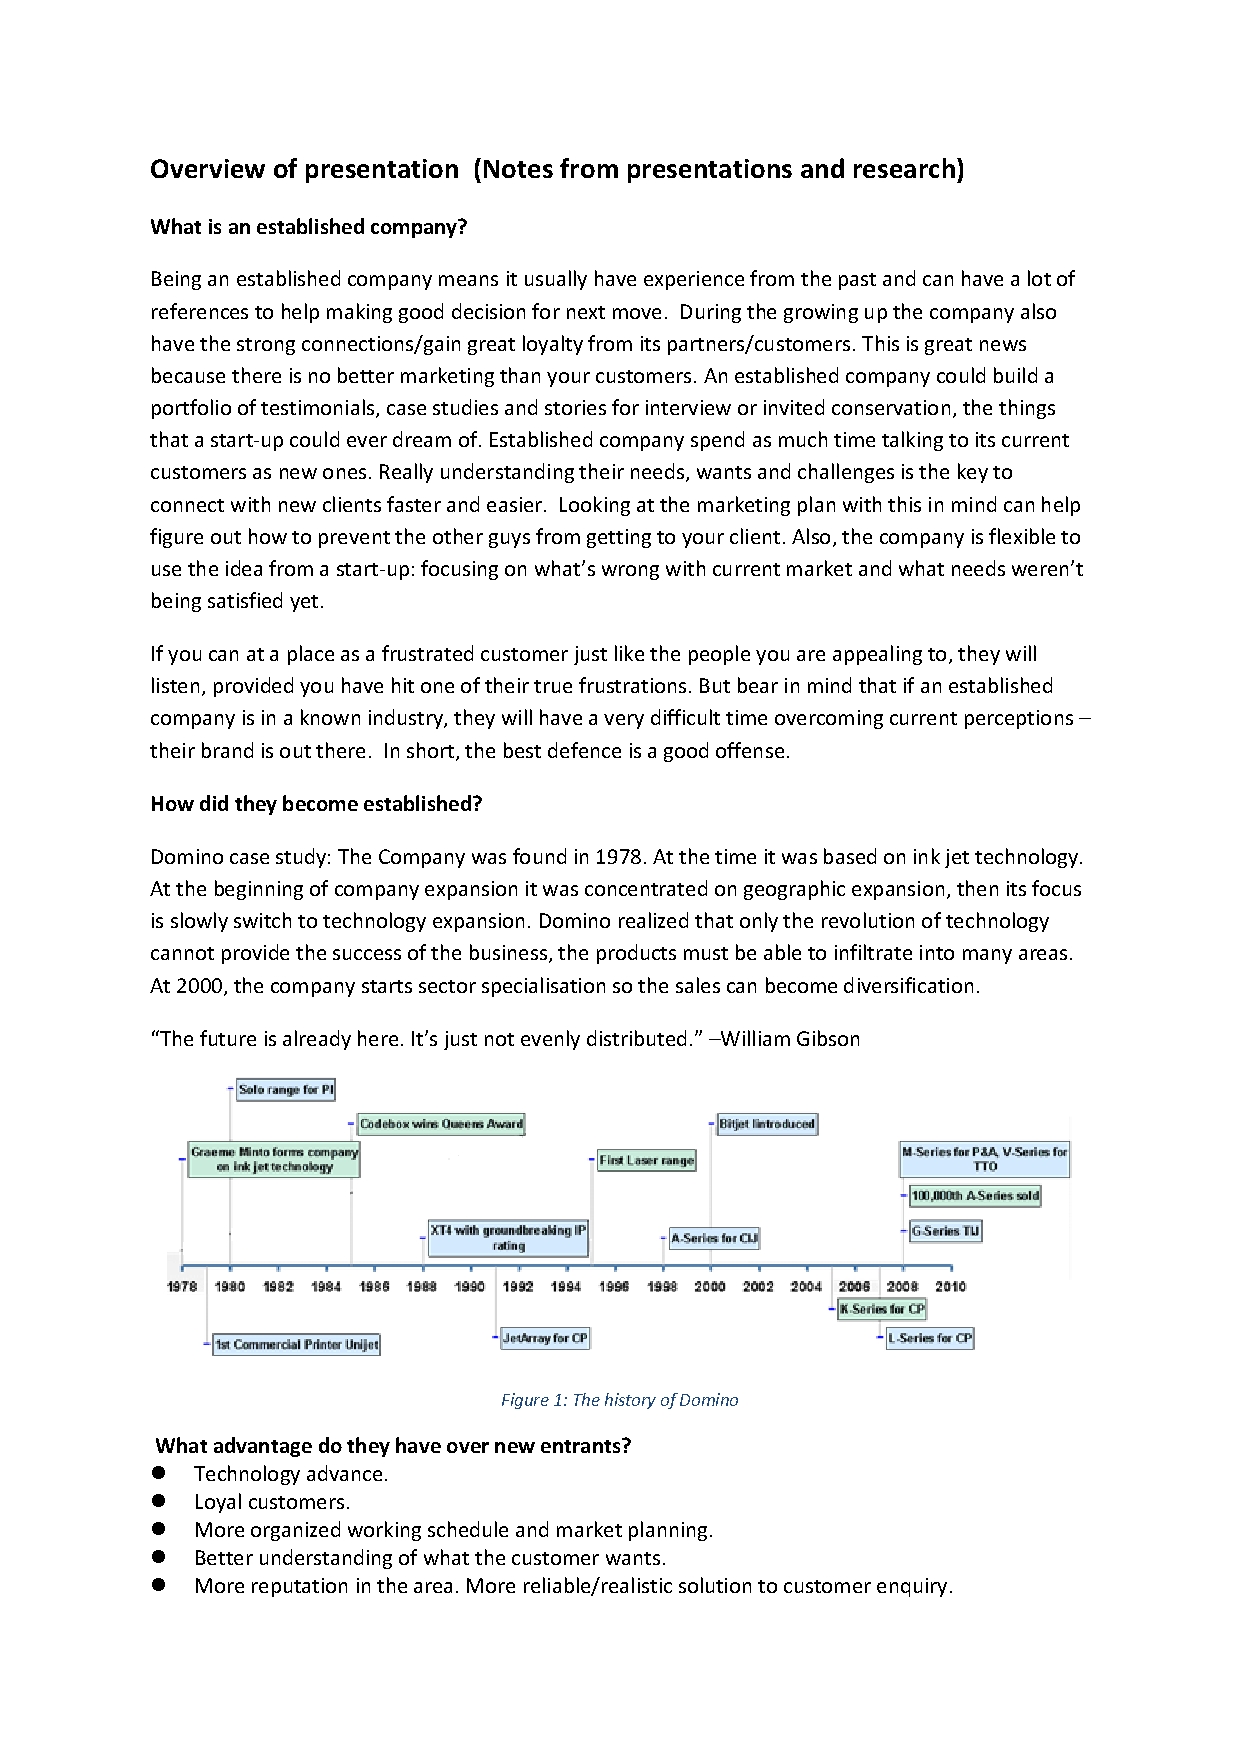
\includegraphics[width = 0.9\textwidth]{Figures/Overview_of_presentations}
		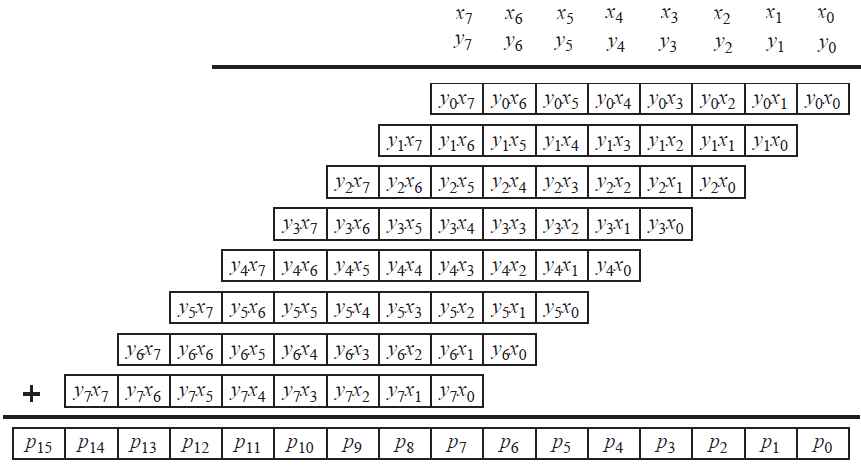
\includegraphics[width = \textwidth]{Figures/multiplier}		
		\caption{Explaination of combinational multiplier \cite{mux}}
		\label {fig:combinational multiplier}
\end{figure}
\newpage

In this project, only the integers are involved in the addition. But the matrix coefficients for the multiplication in the affine transform are 2’s complement signed fixed‐point fractions, which have the radix point positioned after the most significant bits. Therefore the fifteenth and eighth bits of the multiplication result were extracted in order to represent the correct integer of the calculation, and the fraction part was discarded entirely.  The weight of the leading bit of the truncated representation is considered as \(-2^7\) so both positive and negative number can be correctly represented.\\\\
The testbench of ALU is shown in listing~\ref{ALU}. ALU opcode is shown in listing~\ref{alucode}.

\lstset{language=verilog,caption={alucode.sv},label=alucode}
\begin{lstlisting}
// alu function bits
`define Fsize  2

`define RA   2'b00
`define RB   2'b01
`define RADD 2'b10
`define RMUX 2'b11
\end{lstlisting}

\lstset{language=verilog,caption={Arithmetic Logic Unit testbench},label=ALU}
\begin{lstlisting}
`include "alucodes.sv"  
module alutest;
  parameter n =8; // data bus width
  logic signed[n-1:0] a, b; // ALU input operands
  logic [`Fsize-1:0] func; // ALU function code
  logic [n-1:0] result; // ALU result

alu  #(.n(n)) r(.*);

//------------- code starts here ---------
initial
begin
  a= 8'b11100000;
  b= 8'b00010100;
		
  // test all functions
  #10 func = `RA;     // result = a
  #10 func = `RB;     // result = b
  #10 func = `RADD;   // result = a+b 
  #10 func = `RMUX;   // result = a*b
	
end
endmodule 
\end{lstlisting}

\begin{figure}[H]
		\centering
		%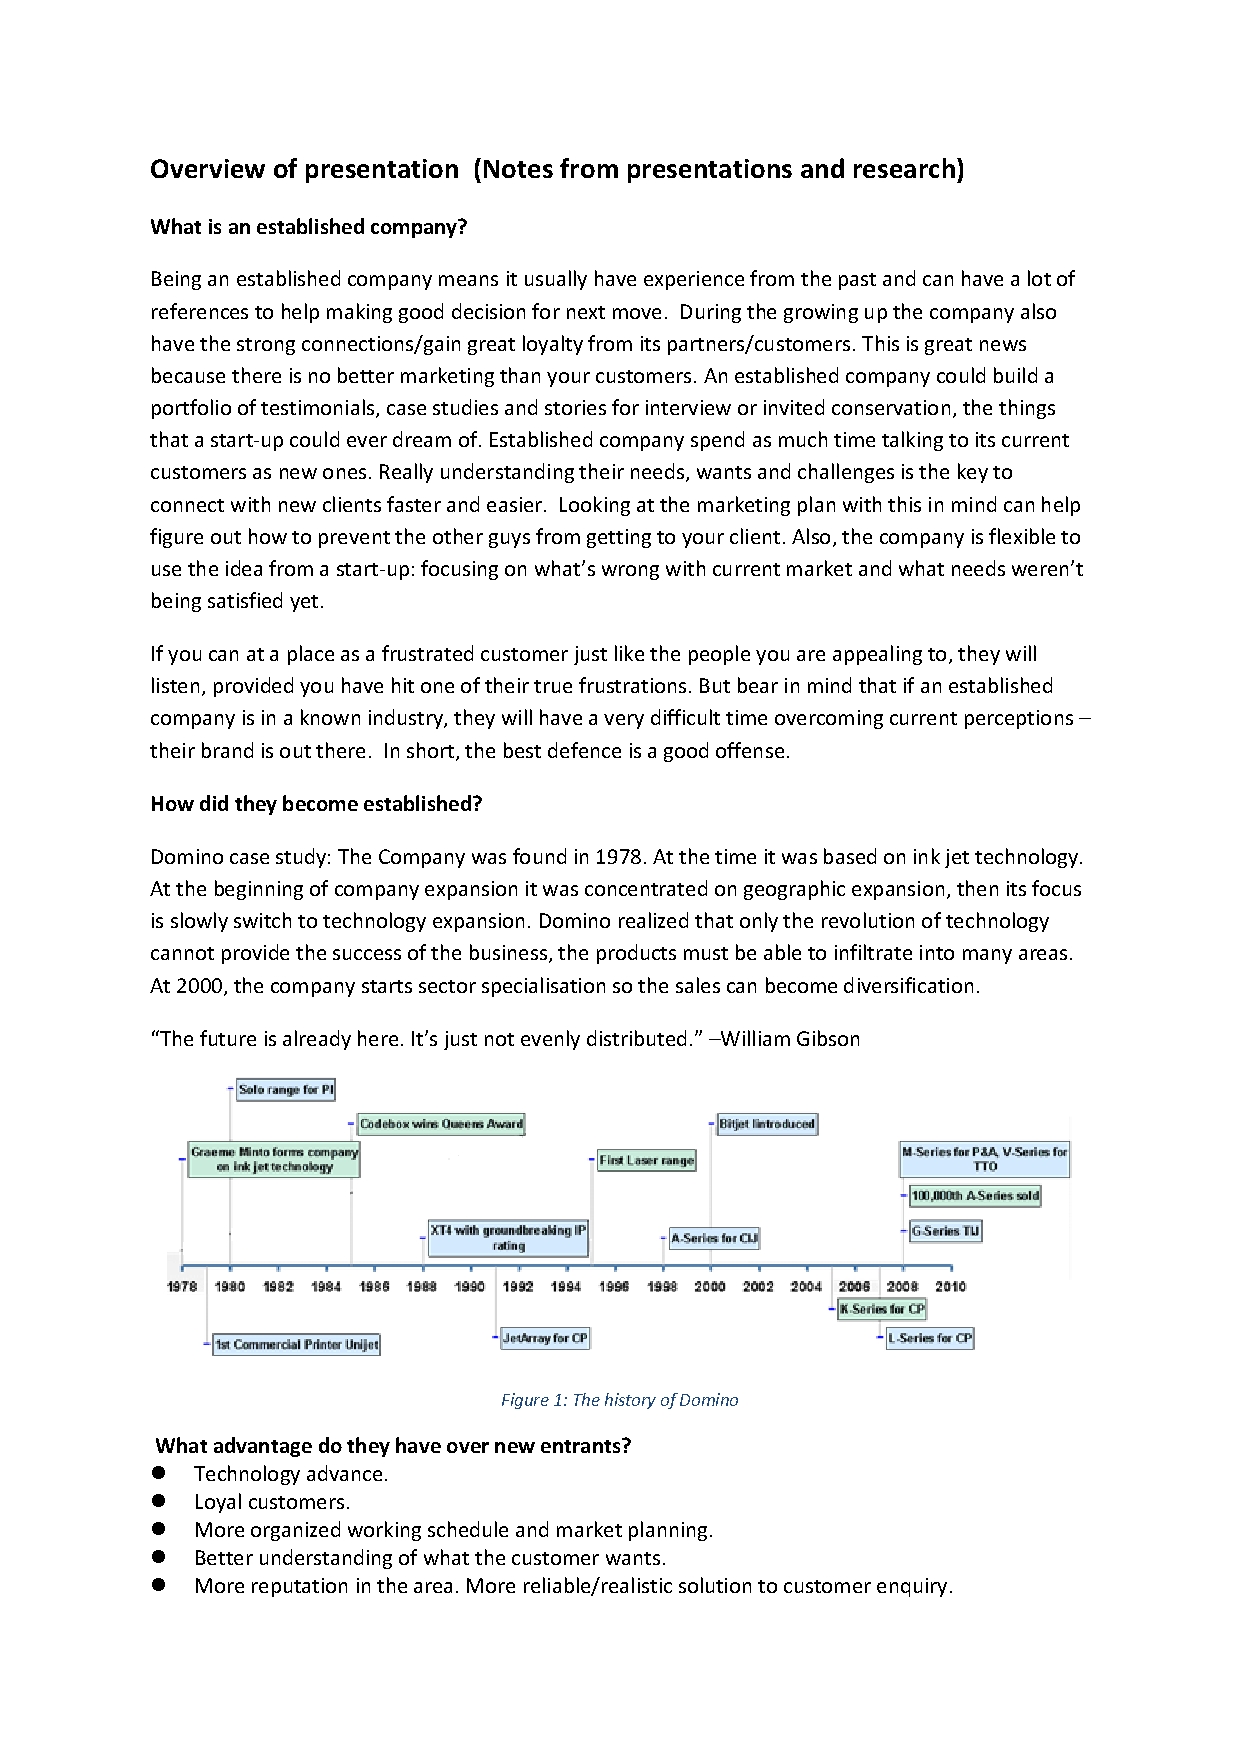
\includegraphics[width = 0.9\textwidth]{Figures/Overview_of_presentations}
		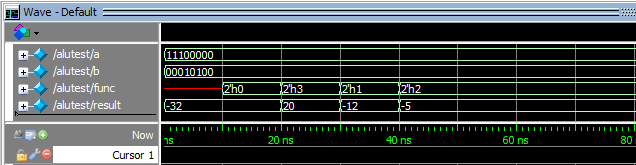
\includegraphics[width = \textwidth]{Figures/ALU}		
		\caption{Simulation results of Arithmetic Logic Unit}
		\label {fig:ALUtest}
\end{figure}

The testbench simulated Pass-the-ALU, addition and multiplication function with two numbers. Number A was considered as -0.25 for a fractional number or -32 for an integer and B was treated only as 20 for an integer. At the 10ns and 20ns, the ALU was commanded to pass -0.25 and 20 without any calculation. At the 30ns, an addition was executed and -12 was the result of -32 plus 20. At the 40ns, -5 was shown as the result of a multiplication between -0.25 and 20. The manual calculation confirmed the ALU test results were all correct.\\\\
The RTL synthesis of ALU is shown in Figure~\ref{fig:ALU}. The ALU is quite compact without other redundant arithmetic logics. The multiplier is synthesised as an embedded hardware unit of Altera Cyclone III.

\begin{figure}[H]
		\centering
		%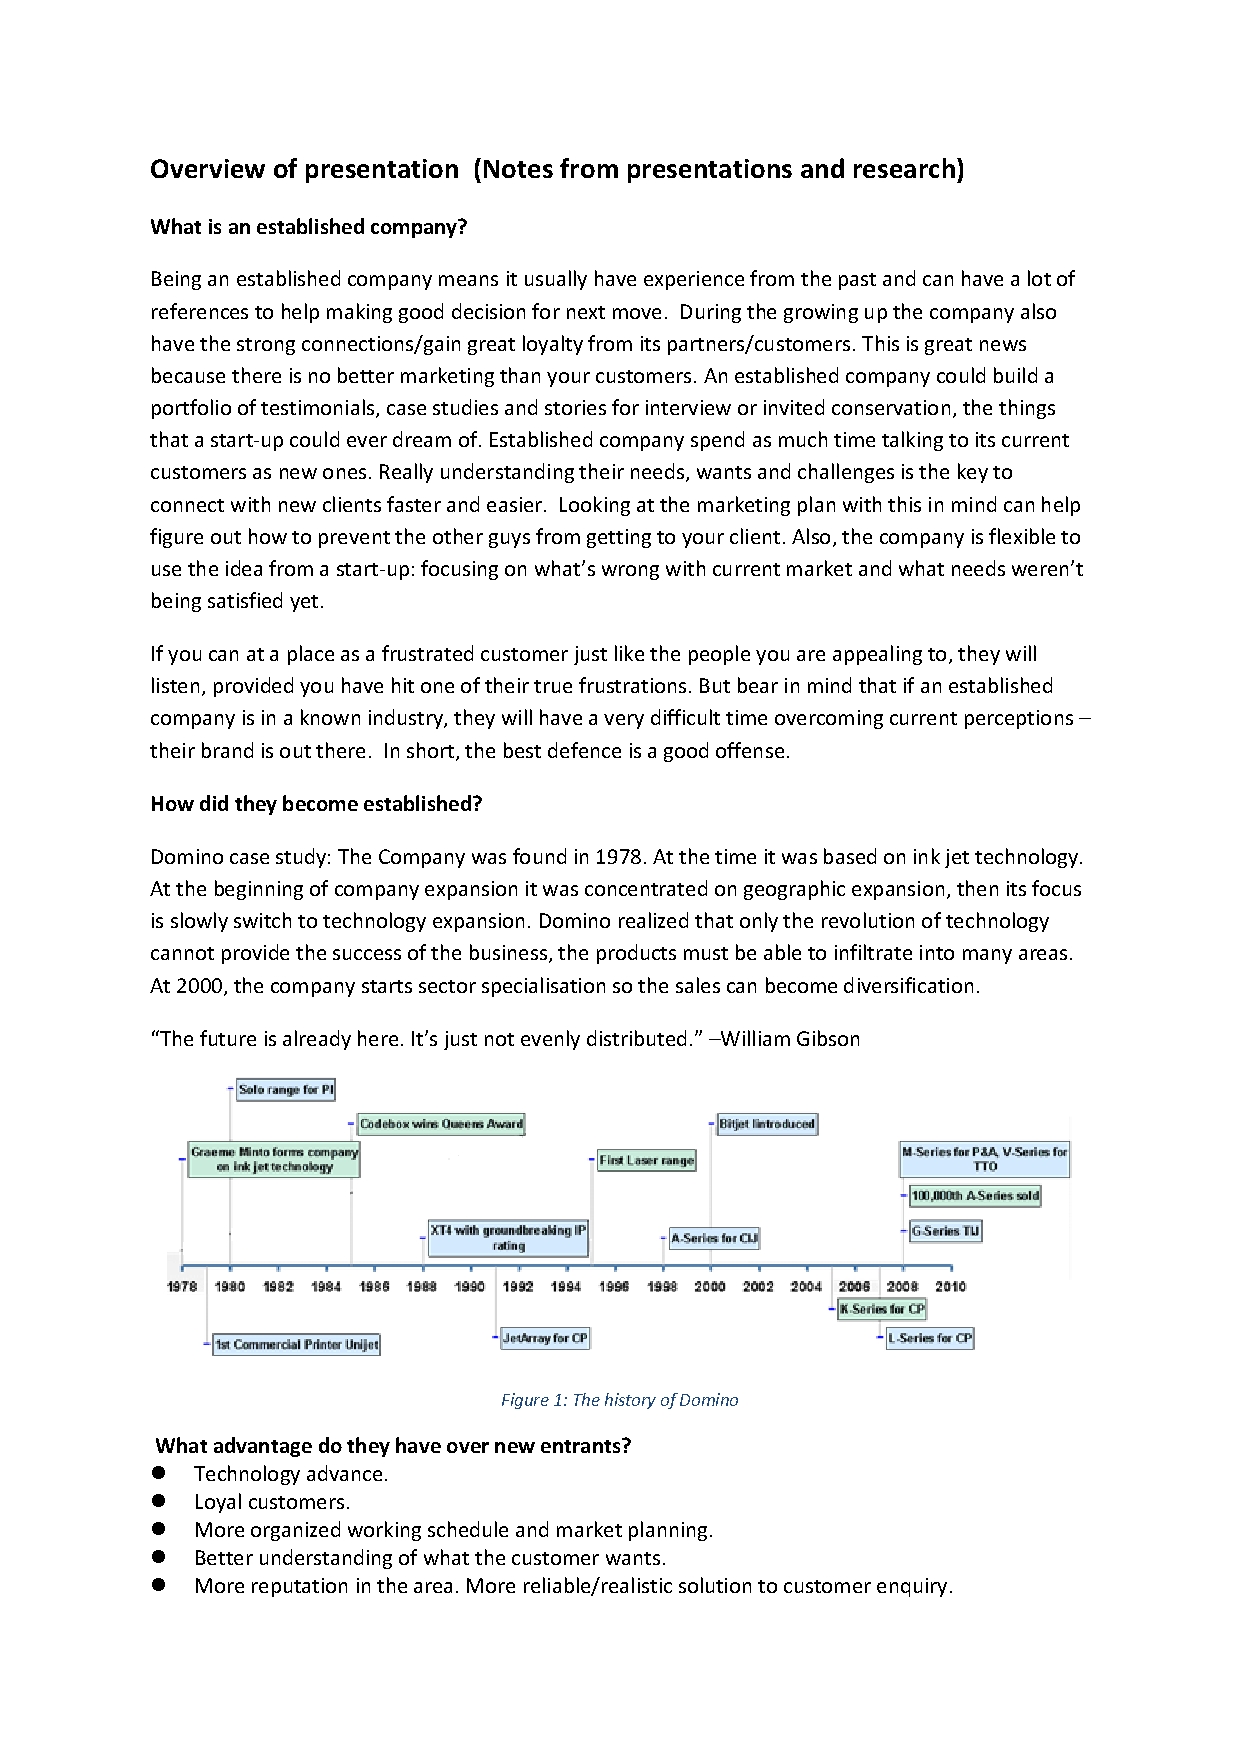
\includegraphics[width = 0.9\textwidth]{Figures/Overview_of_presentations}
		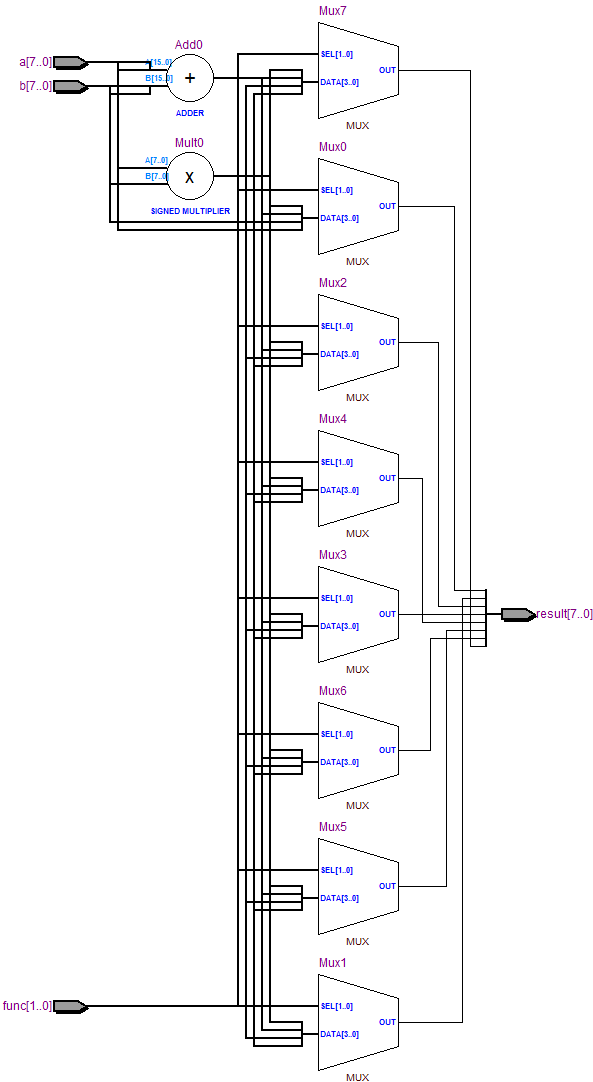
\includegraphics[width = 0.6\textwidth]{Figures/aluu}		
		\caption{RTL synthesis of Arithmetic Logic Unit}
		\label {fig:ALU}
\end{figure}

\section{Altera DE0 implementation and optimization} \label{Altera DE0 implementation}
\subsection{Original design DE0 implementaion}
A top level picoMIPS CPU module was implemented to encapsulate all sub-level individual modules. The CPU reads ten switches SW [9:0] from FPGA device, and outputs the results directly to the LEDs to save some hardware. Additional multiplexer \textit{imm} selects the data between immediate bits and source register output, and the multiplexer \textit{sel} selects switches [7:0] or ALU output. A simple counter \cite{slowcounter} was added to slow down the Altera DE0 embedded 50MHz clock to around 10Hz for the demonstration of the design.\\\\
The testbench for the complete CPU is shown in listing~\ref{cputest}. A pixel coordinates [16 20] were used as the example in the simulation.\\\\
\lstset{language=verilog,caption={Testbench for CPU},label=cputest}
\begin{lstlisting}
module cputest;
parameter n = 8;
logic clk;                               //counter clock
logic [9:0] SW;                          //input SW 
logic[n-1:0] outport;                    //output port (ALU output)
logic reset;                             //master reset

// ALU
logic [1:0] ALUfunc;                     // ALU function
logic imm;                               // immediate operand signal
logic [n-1:0] Alub;                      // output from imm MUX

// registers
logic [n-1:0] Rd, Rs, WdataALU, Wdata;   // Register data
logic w;                                 // register write control

// Program Counter  
parameter Psize = 5;                     // up to 32 instructions
logic PCincr,PCabsbranch;                // program counter control
logic [Psize-1 : 0]ProgAddress;          // program memory address

// Program Memory
parameter Isize = n+10;                  // Isize - instruction width
logic [Isize-1:0] I;                     // I - instruction code (hex)

cpu2  #(.n(n)) mydesign(.*);

//------------- code starts here ---------
initial
begin
  clk =  0;
  #5ns  forever #5ns clk = ~clk;
end

initial
begin
  SW[9:0] = 10'b1000000000;  
  #50ns SW[9] = 0;
  #50ns SW[7:0] = 8'b00010000;            //x1
  #50ns SW[8] = 1;
  #50ns SW[8] = 0;
  #50ns SW[7:0] = 8'b00010100;            //y1
  #50ns SW[8] = 1;  
  #50ns SW[8] = 0;
  #50ns SW[8] = 1;
  #50ns SW[8] = 0;                        //stop the processor to start a new calculation
end
endmodule 
\end{lstlisting}

\begin{figure}[H]
		\centering
		%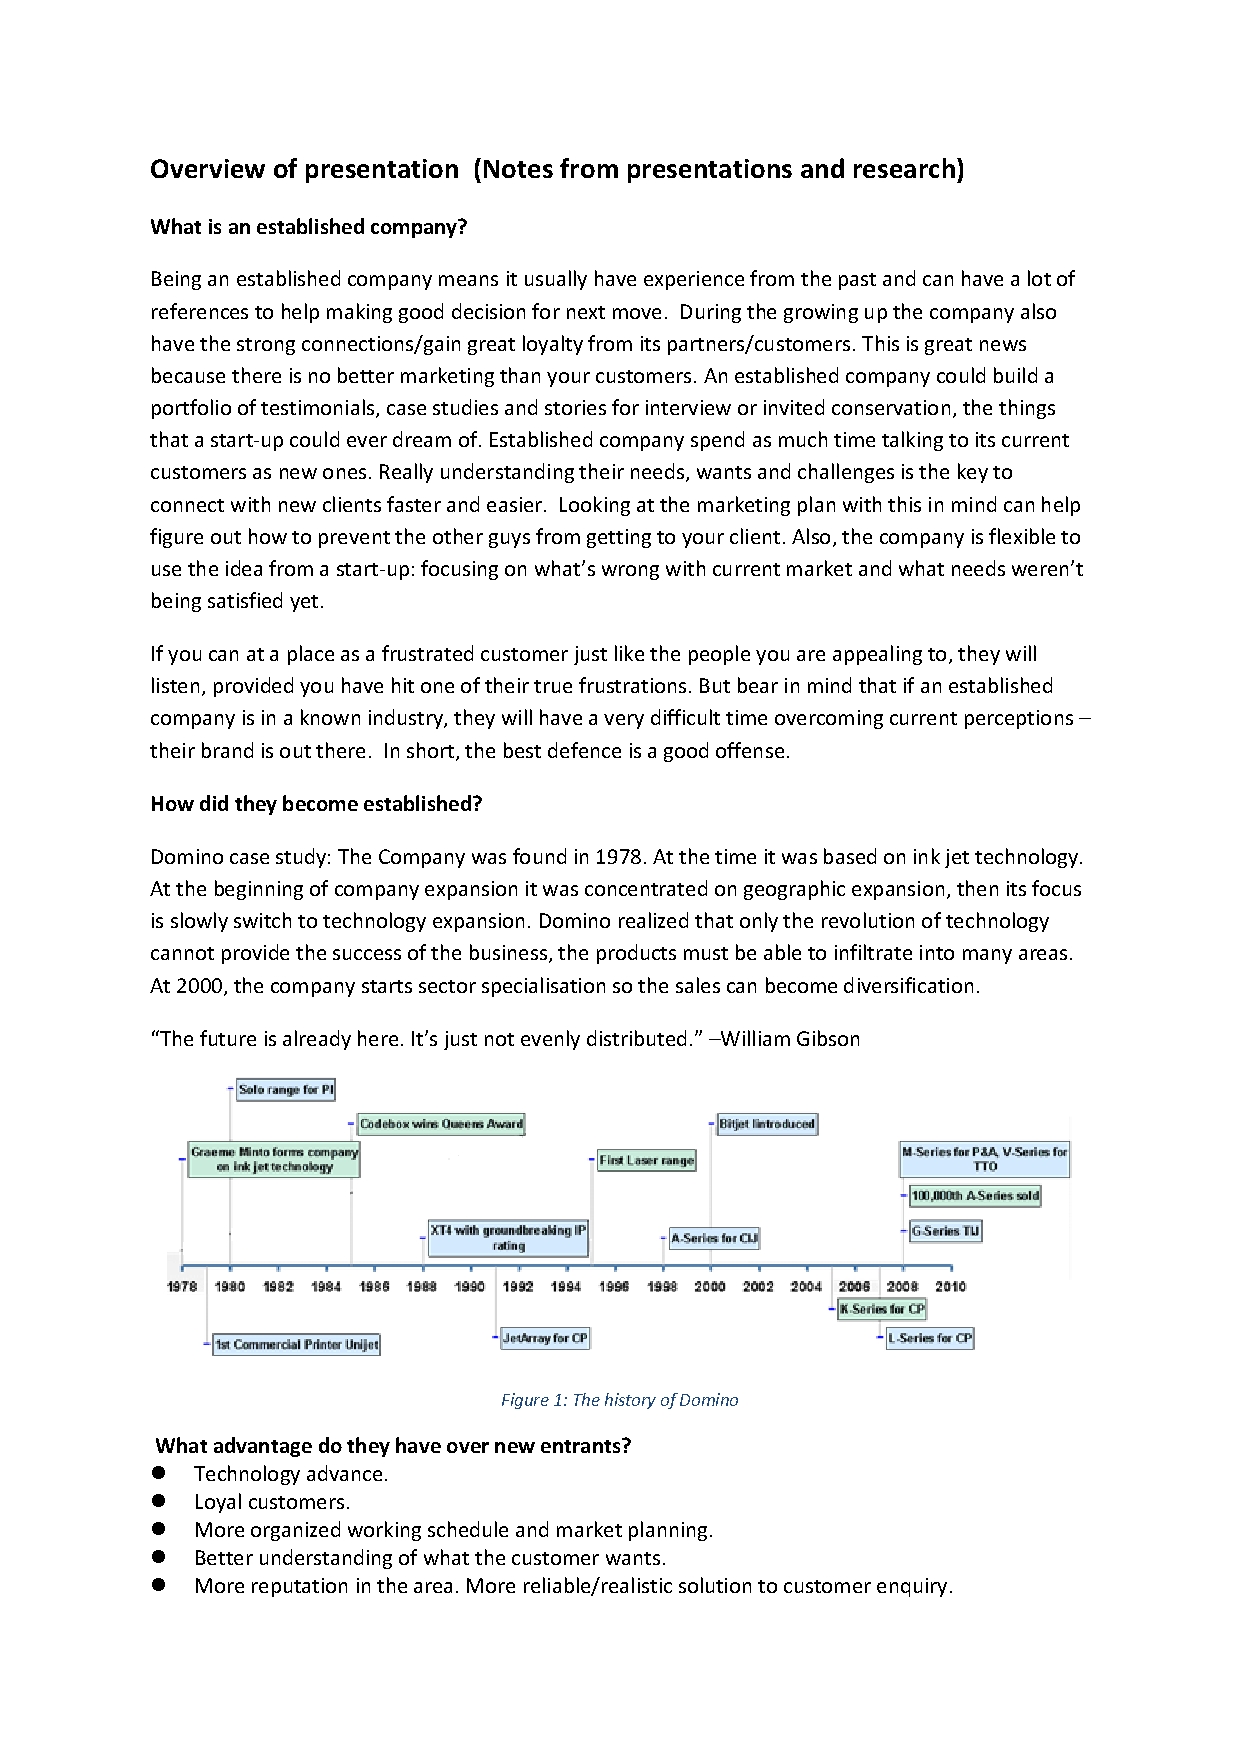
\includegraphics[width = 0.9\textwidth]{Figures/Overview_of_presentations}
		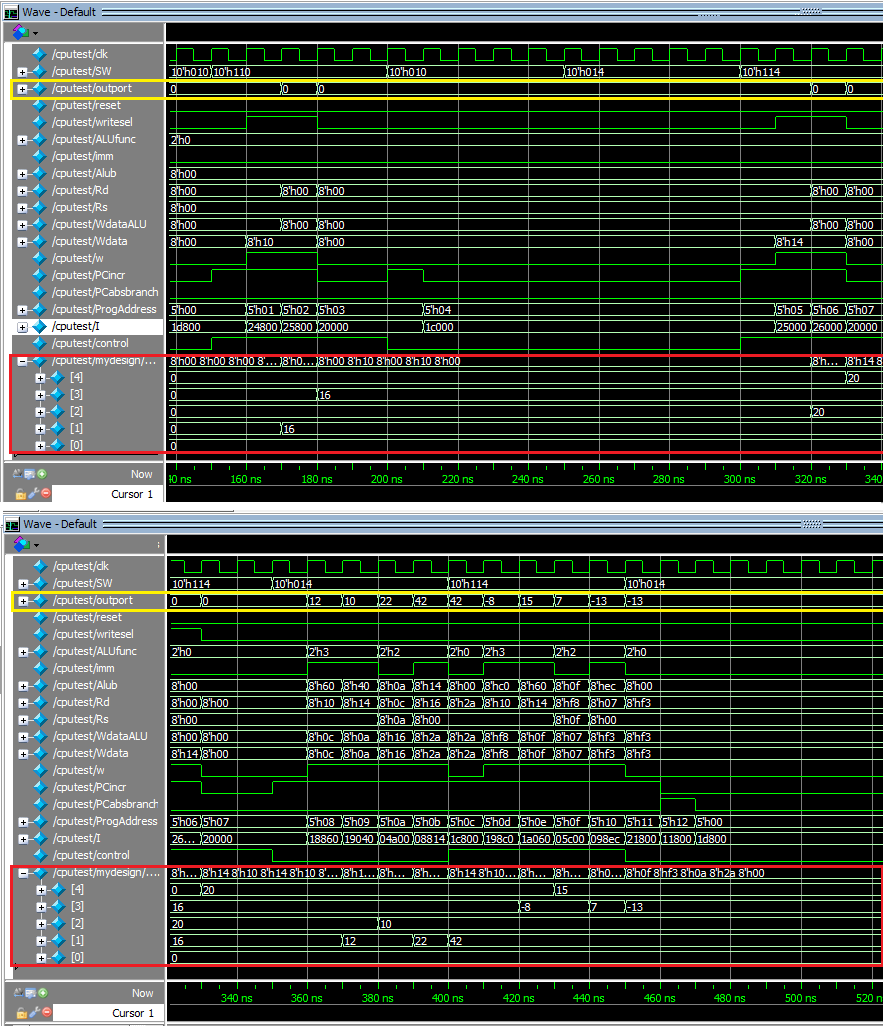
\includegraphics[width = \textwidth]{Figures/original_CPU}		
		\caption{Simulation result of original CPU. (register values in the red box, output in the yellow box)}
		\label {fig:ocpu}
\end{figure}

As indicated in Figure~\ref{fig:ocpu}, the CPU successfully completed the affine transform. In details, at 150ns and 300ns, the WAIT instructions paused the operation until the required switch signal \textit{control (SW[8])} has appeared. The coordinates were correctly loaded into the register with LOAD instruction at 160ns and 310ns. The transform started from 360ns. It was executed by a series of addition and multiplication and output result was checked correct with manual calculation (at 390ns and 440ns).\\\\
The CPU module was synthesised by software \textit{Quartus II}. It was then programmed into chip EP3C16F484C6 (Cyclone III) on FPGA through the Quartus II programmer. The CPU modules was also re-synthesised using Cyclone IV E as the target to obtain the cost figure. For the FPGA test, the test coordinates were exactly the same as in the testbench. After the algorithm, the LEDs outputted the same results from the testbench, as shown in Figure~\ref{fig:fpga}.

\begin{figure}[H]
		\centering
		%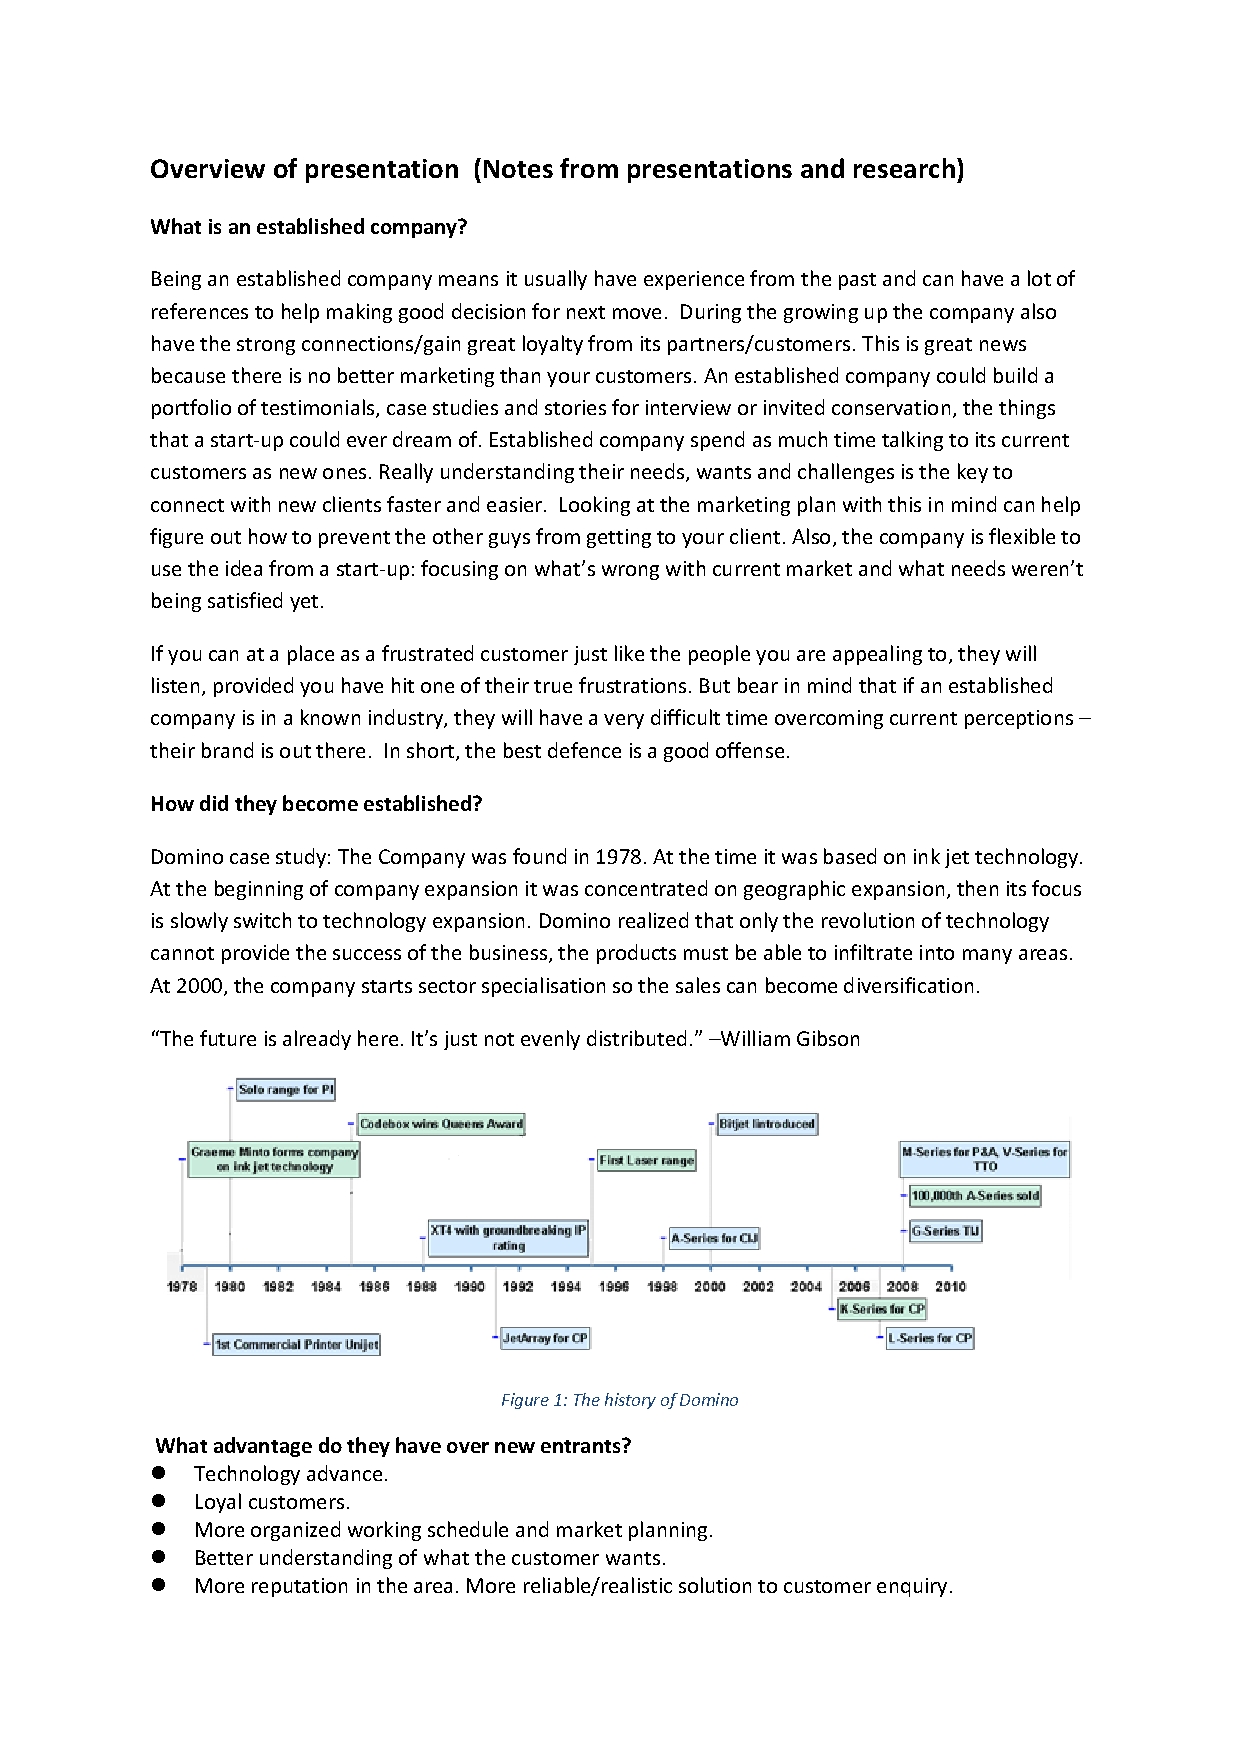
\includegraphics[width = 0.9\textwidth]{Figures/Overview_of_presentations}
		\includegraphics[width = \textwidth]{Figures/FPGA}		
		\caption{\textit{Left}: x\textsubscript{2} = 42 (00101010) \textit{Right}: y\textsubscript{2} = -13 (11110011)}
		\label {fig:fpga}
\end{figure}

Although the original picoMIPS processor successfully performed the affine transform, the cost figure was unsatisfying high (Figure~\ref{fig:cputest}). The general purpose register occupied the most logic units in the design, and long instruction length also enlarge the program counter and memory. Thus they were the major targets at the optimization stage.

\begin{figure}[H]
		\centering
		%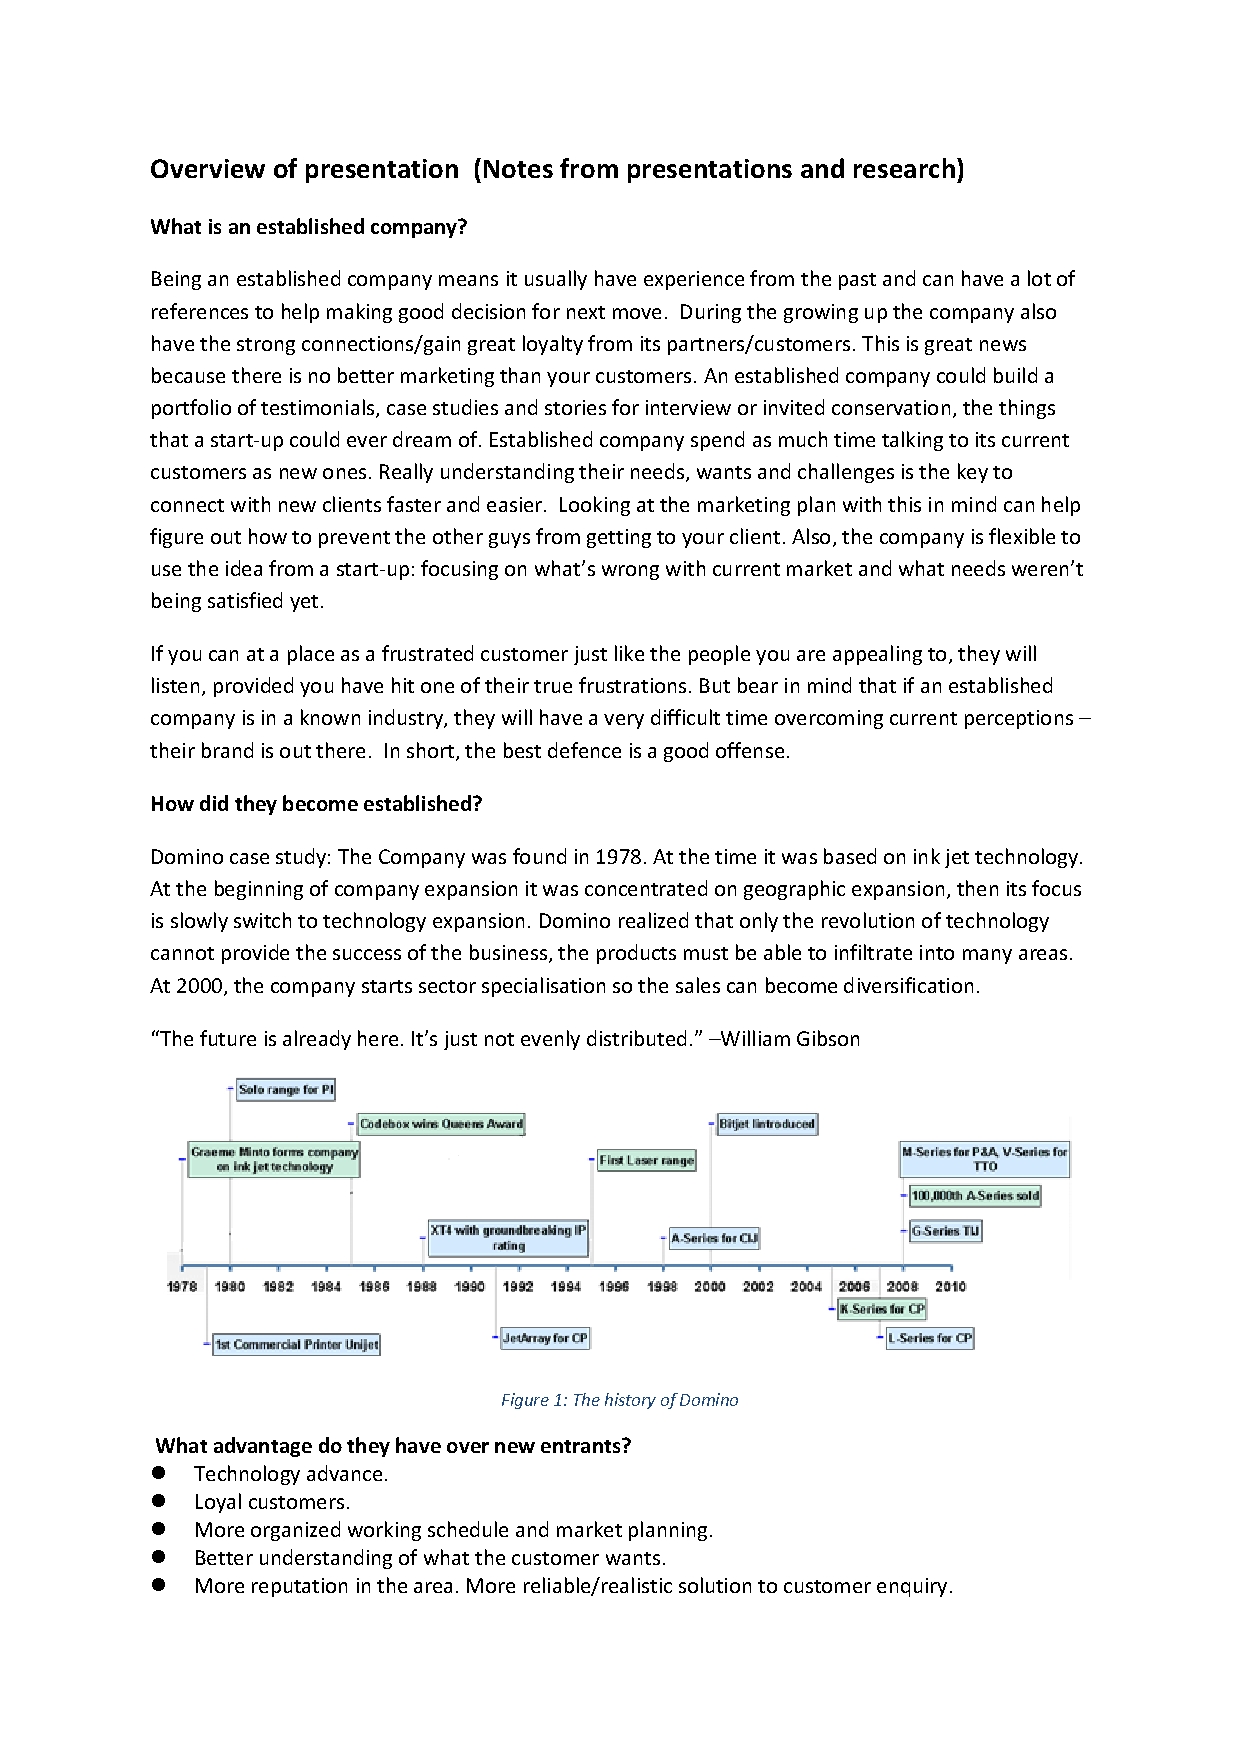
\includegraphics[width = 0.9\textwidth]{Figures/Overview_of_presentations}
		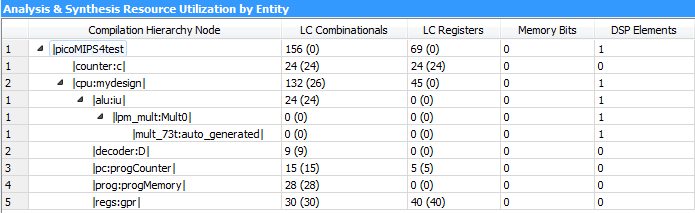
\includegraphics[width = \textwidth]{Figures/ocpucost}		
		\caption{synthesis statistics of the original CPU}
		\label {fig:cputest}
\end{figure}

\subsection{General purpose register optimization}

Using the embedded memory in the FPGA could significantly reduce the usage of combinational logic in the register. However, it is synchronous. Therefore the asynchronous read was replaced by synchronous one in the systemverliog file to describe new register. In total there were ten registers declared, although only four registers were used in the affine transform. Otherwise the synthesis tool would prefer to use combinational logics rather than the embedded memory to build the desgin. 

\begin{figure}[H]
		\centering
		%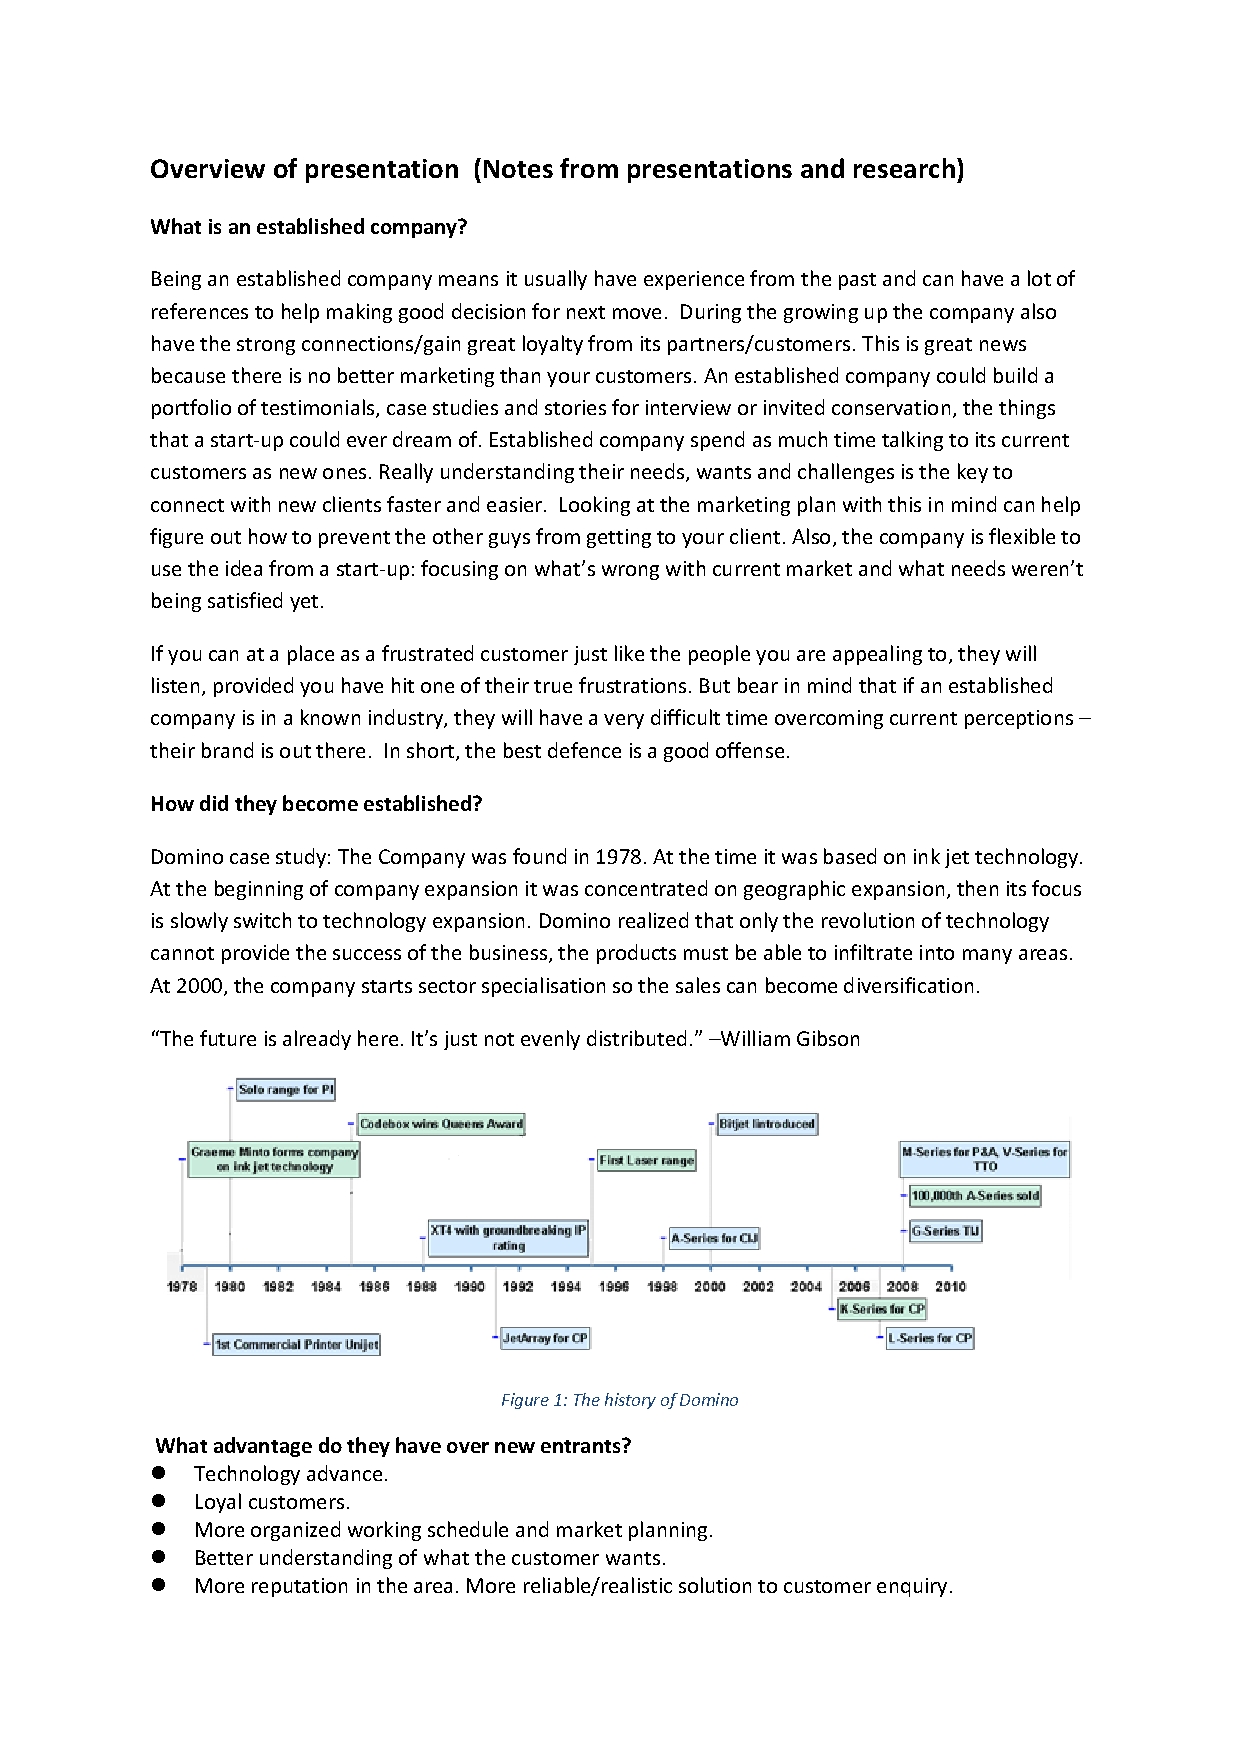
\includegraphics[width = 0.9\textwidth]{Figures/Overview_of_presentations}
		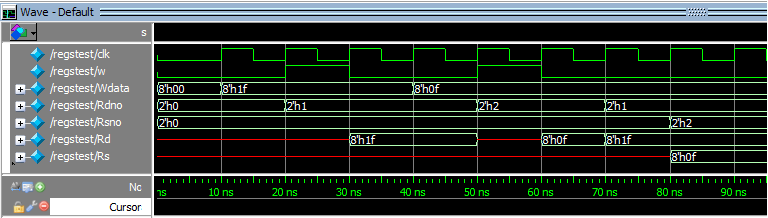
\includegraphics[width = \textwidth]{Figures/newGPR}		
		\caption{Simulation results of the new General Purpose Register}
		\label {fig:newGPRtest}
\end{figure}

The testbench for the new register is identical to the original one. However the simulation result from Figure~\ref{fig:newGPRtest} indicates that the register requires two clock cycles to output the newly written data due to the synchronous read (at 20nns and 50ns). During the affine transform, this behaviour will cause correct calculation result from ALU to appear only after the second clock cycle. 
As the result, the new register was synthesised as one embedded 32 bits memory block with no extra logic units used, as shown in Diagram~\ref{fig:newregister}.

\begin{figure}[H]
		\centering
		%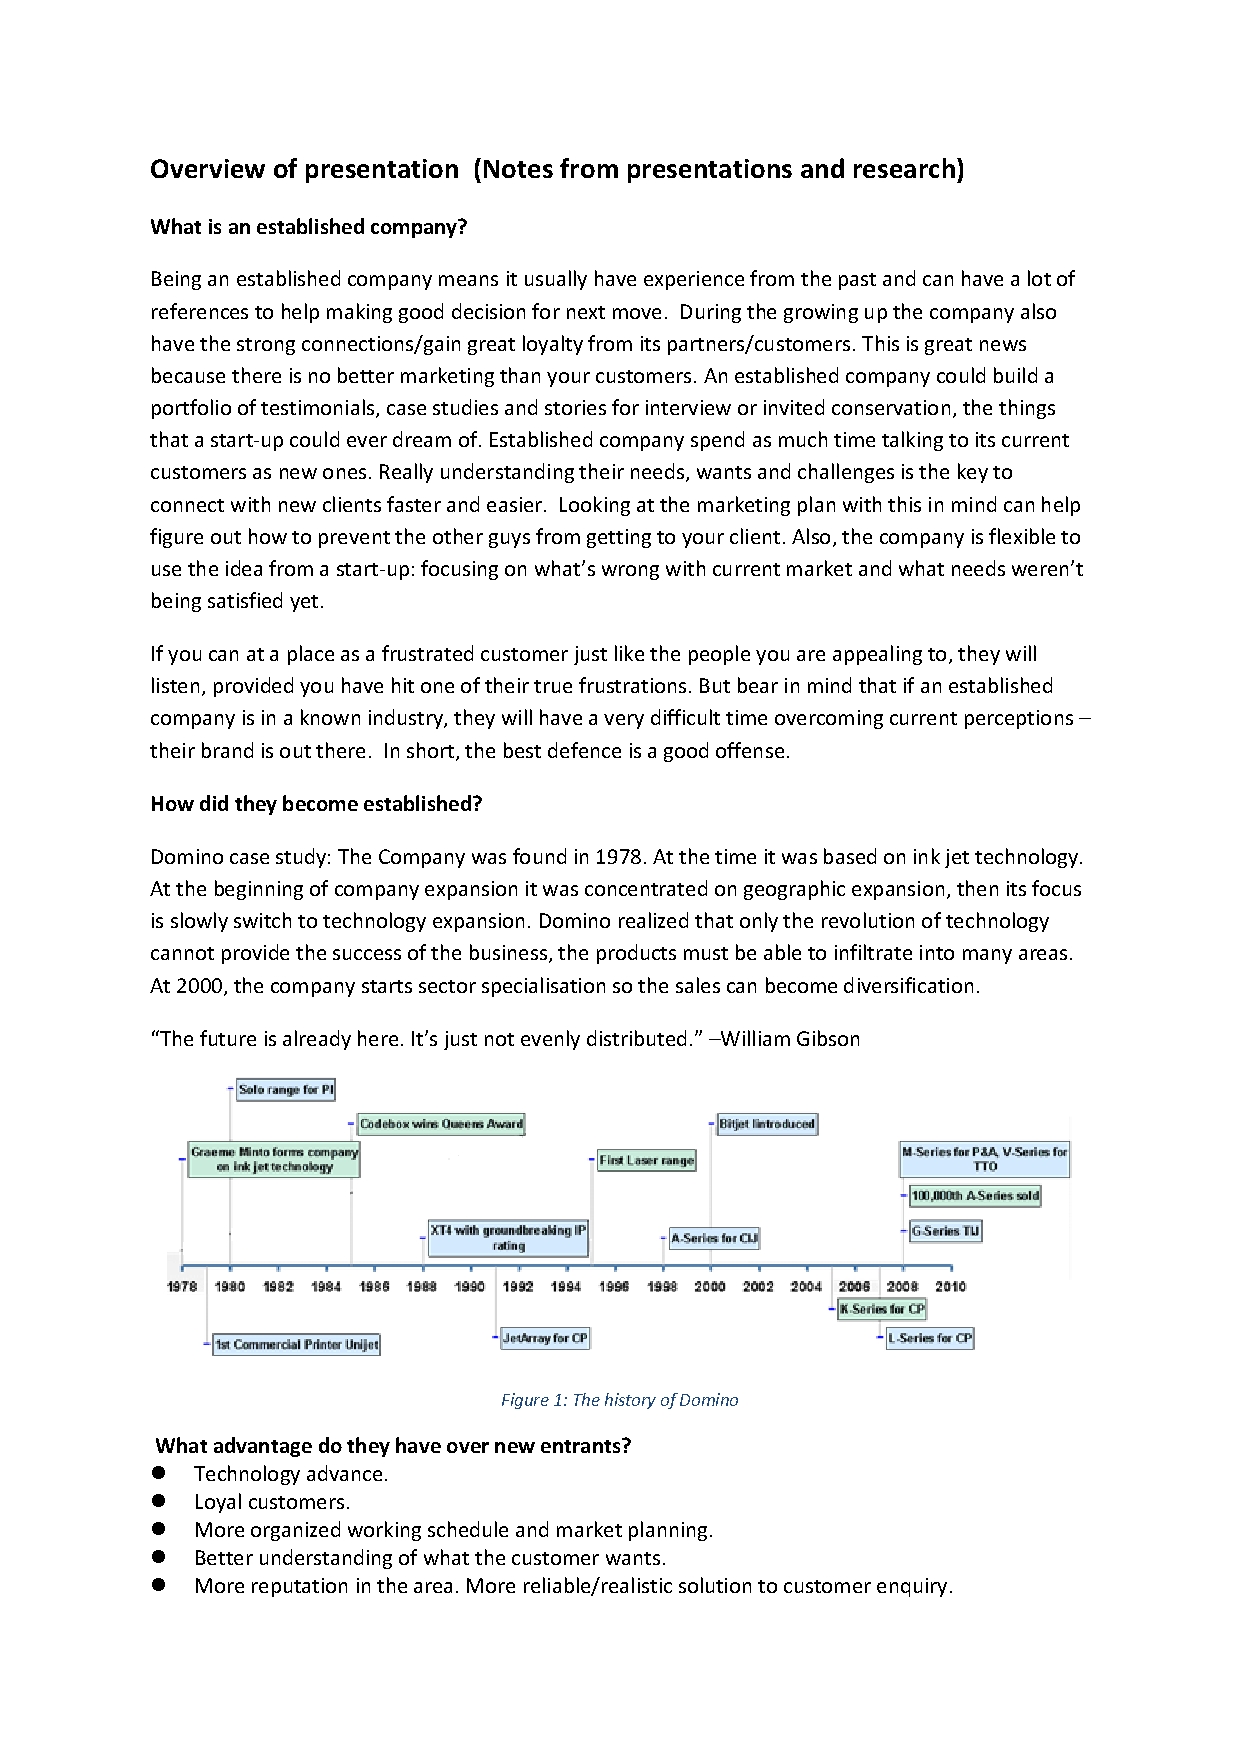
\includegraphics[width = 0.9\textwidth]{Figures/Overview_of_presentations}
		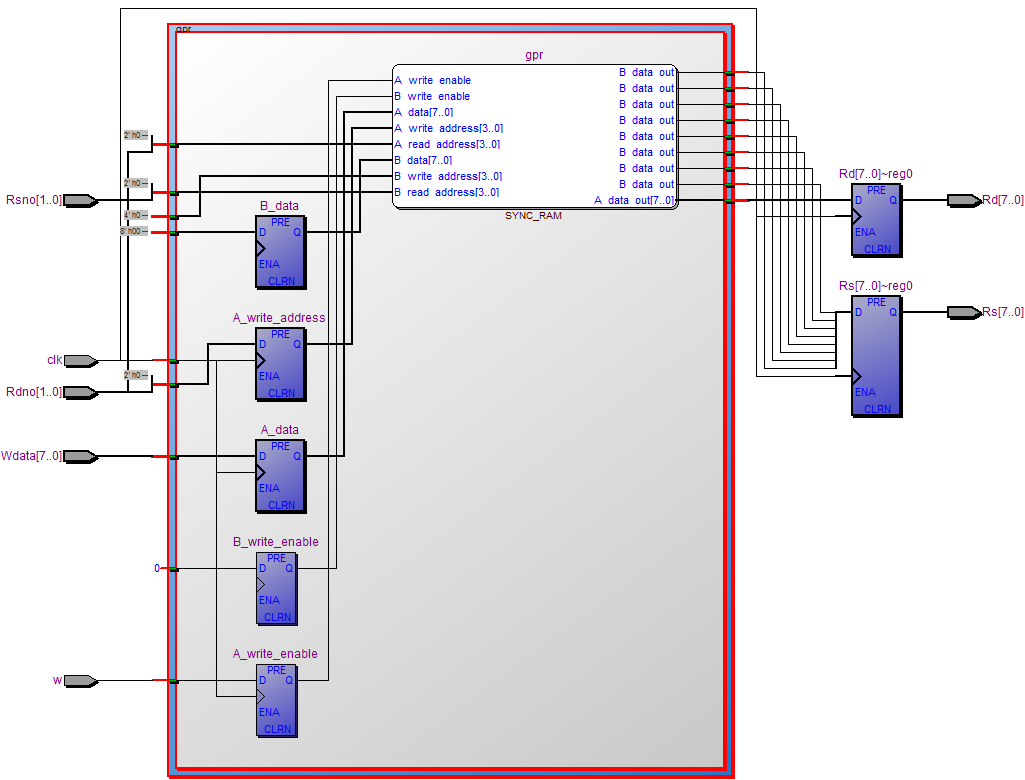
\includegraphics[width = \textwidth]{Figures/newregs}		
		\caption{RTL synthesis of the new General Purpose Register}
		\label {fig:newregister}
\end{figure}
\newpage

\subsection{Decoder optimization}
A two-stage state machine (listing~\ref{newdecoder}) was added to the original decoder to address the problem caused by the new register. 
\lstset{language=verilog,caption={state machine part of the new decoder code},label=newdecoder}
\begin{lstlisting}
module decoder
.....
always_ff @ (posedge clk or posedge reset)
begin
  if (reset)
      state = `FETCH;
  else
  begin
    case(state)
      `FETCH: state <= `EXECUTE;
      `EXECUTE: state <= `FETCH;
    endcase
  end
end
.....

endmodule 
\end{lstlisting}

The write-register signal will rise only at \textit{EXECUTE} state to ensure the register could store the correct data, as shown in the Figure~\ref{fig:newDCtest} at 150ns. The PC increment signal will also rise at \textit{EXECUTE} state to avoid the clock cycle mismatch when a \textit{WAIT} instruction moves to the next one, which may happens at 180ns. Additional signal \textit{selfirst} was implemented to select 4bits instruction immediate as the upper part to form the complete 8bits immediate value because of the new instruction format. Otherwise the 4bits immediate will be used as the lower part. It only rises to high in instruction \textit{ADDIF} and \textit{MUXI} (at 220ns and 260ns). 

\begin{figure}[H]
		\centering
		%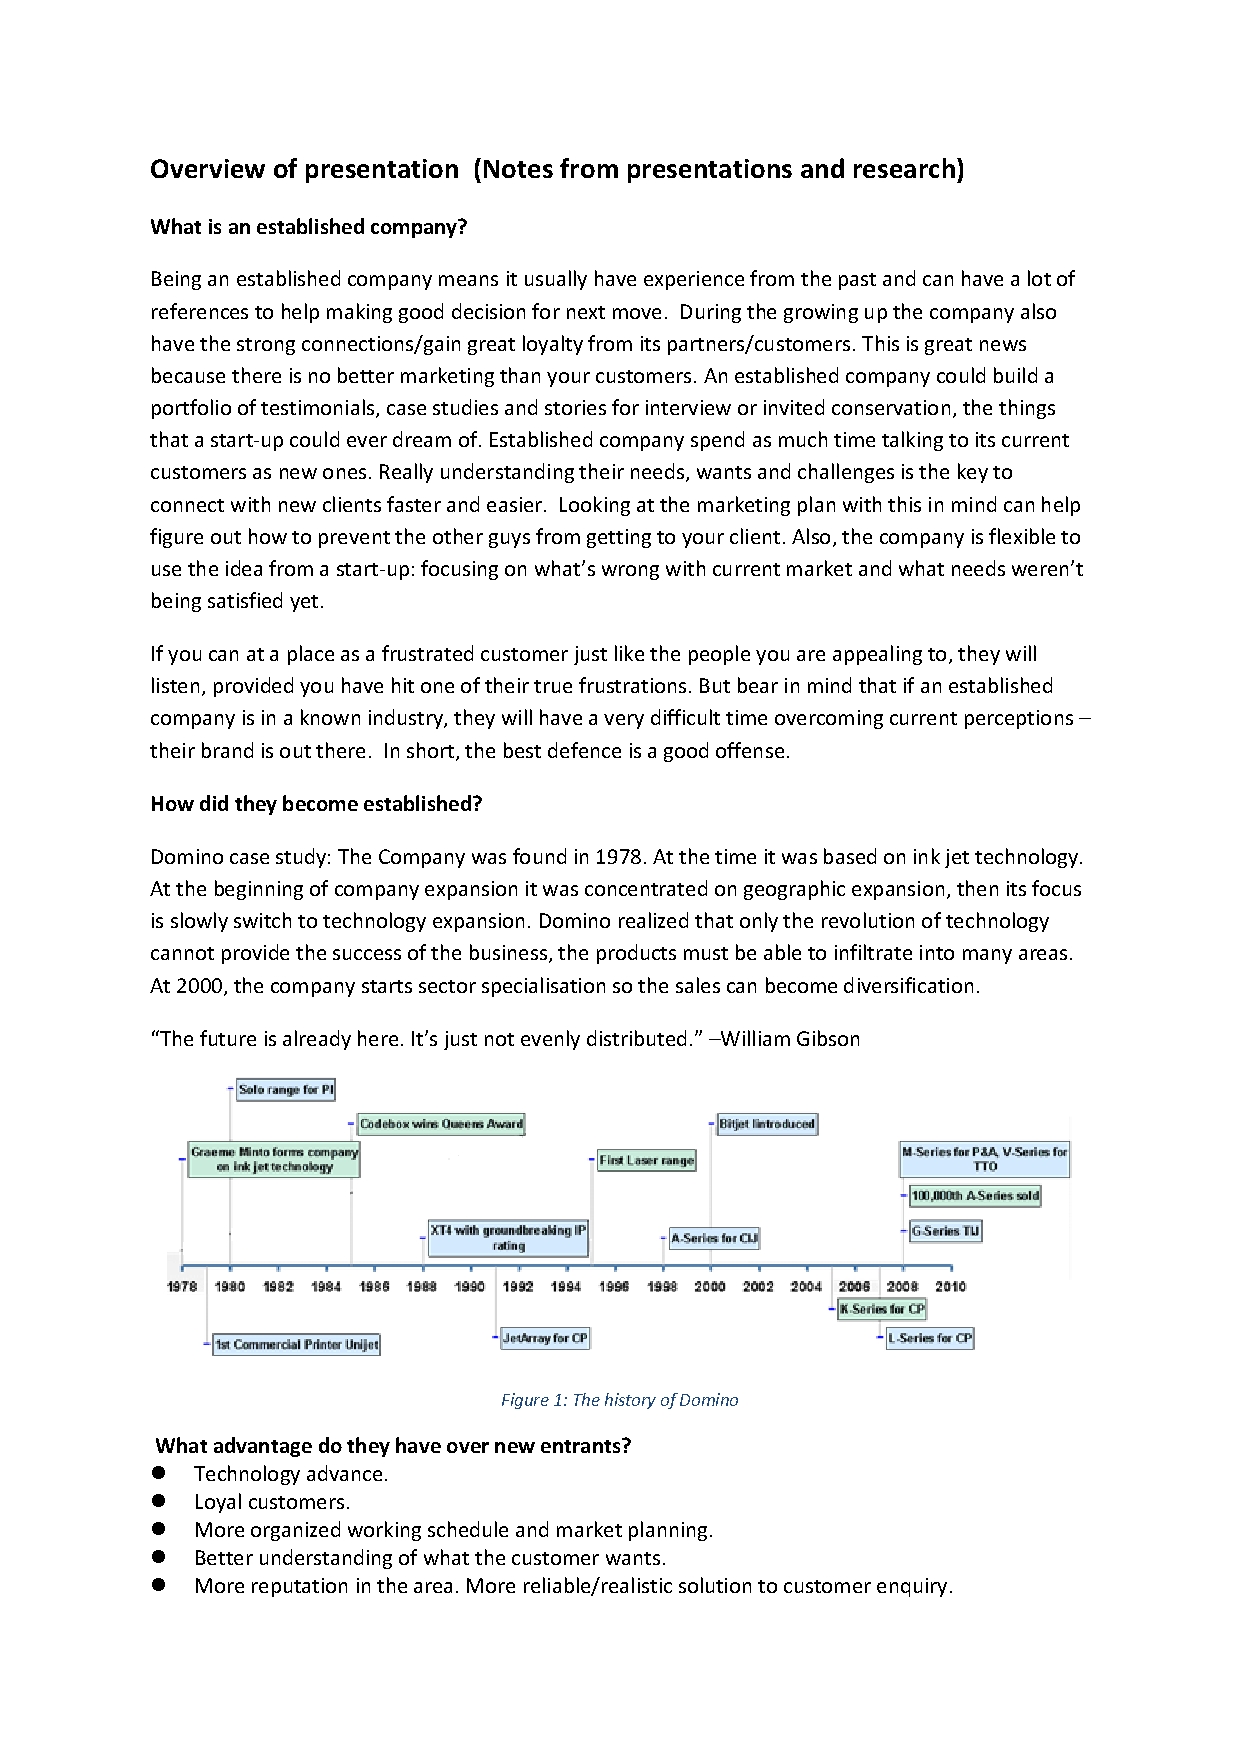
\includegraphics[width = 0.9\textwidth]{Figures/Overview_of_presentations}
		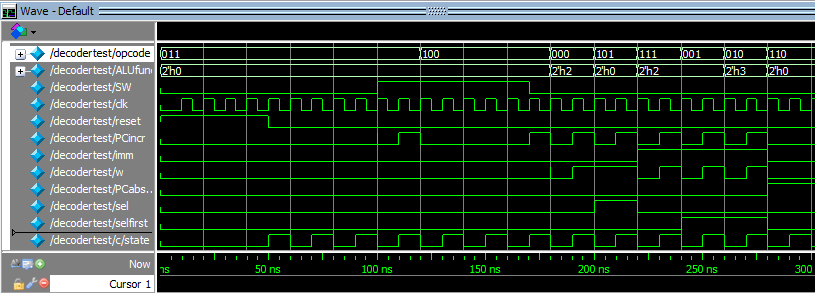
\includegraphics[width = \textwidth]{Figures/newdecodertest}		
		\caption{Simulation results of the new Decoder}
		\label {fig:newDCtest}
\end{figure}

The testbench for the new decoder is shown in listing~\ref{newDCtest}.

\lstset{language=verilog,caption={New Decoder testbench},label=newDCtest}
\begin{lstlisting}
`include "alucodes1.sv"
`include "opcodes.sv"
`include "states.sv"

module decodertest;

logic [2:0] opcode;
logic [1:0] ALUfunc;
logic SW,clk,reset;
logic PCincr,imm,w,PCabsbranch,sel,selfirst;

decoder c(.*);
//------------- code starts here ---------
initial
begin
  clk =  0;
  #5ns  forever #5ns clk = ~clk;
end
initial 
begin
  SW = 0;	
  reset=1;
  opcode =3'b011;//WAIT0
  #50ns reset =0; 
  #50ns SW=1;    
  #20ns opcode =3'b100; //WAIT1
  #50ns SW=0;
  #10ns opcode =3'b000; //ADD
  #20ns opcode =3'b101; //LOAD 
  #20ns opcode =3'b111; //ADDIL
  #20ns opcode =3'b001; //ADDIF
  #20ns opcode =3'b010; //MUXI
  #20ns opcode =3'b110; //JUMP  
  end
endmodule 
\end{lstlisting}

The RTL synthesis of the new decoder is shown in Figure~\ref{fig:newdecoder}. It has an extra state machine.

\begin{figure}[H]
		\centering
		%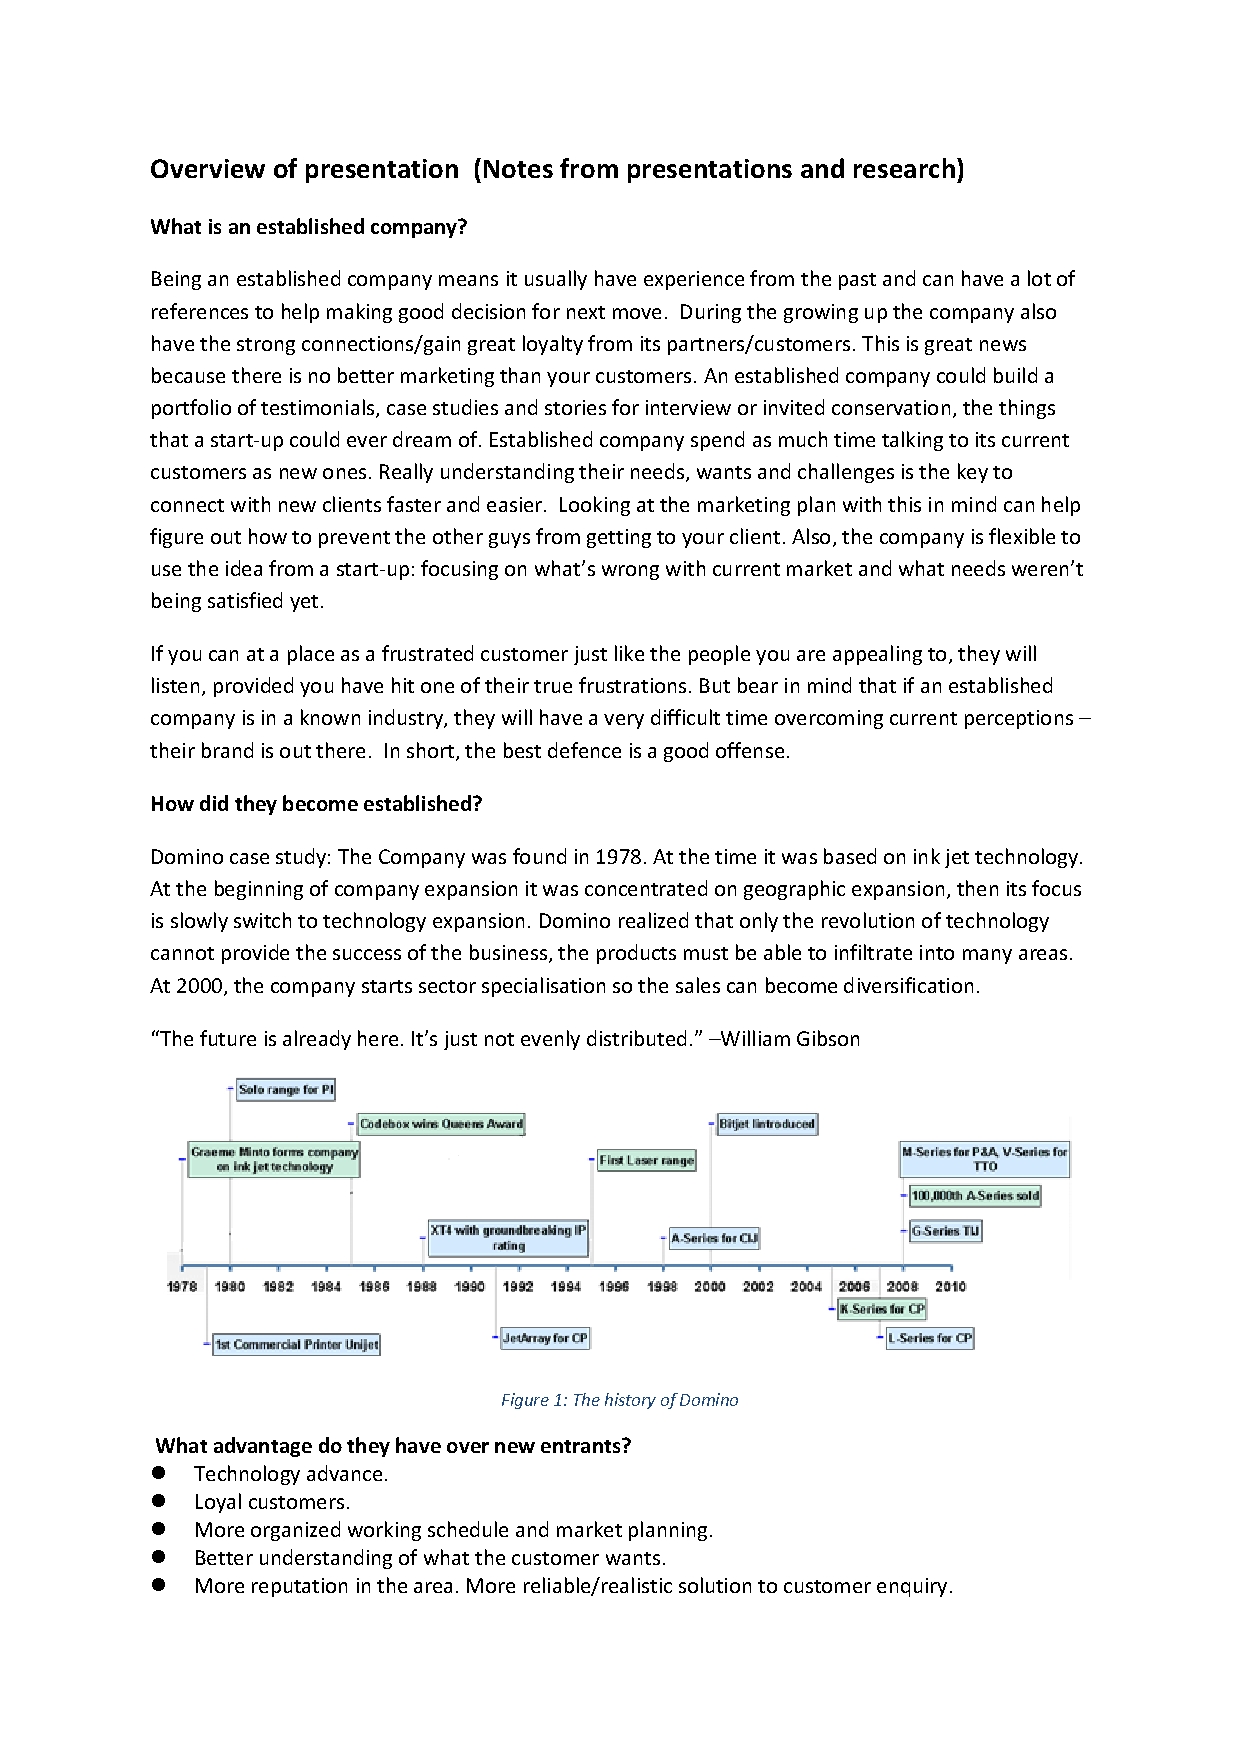
\includegraphics[width = 0.9\textwidth]{Figures/Overview_of_presentations}
		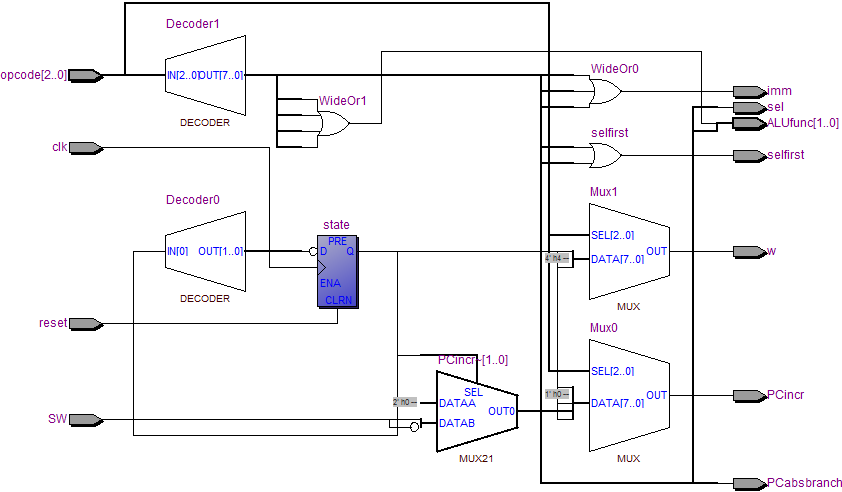
\includegraphics[width = 0.9\textwidth]{Figures/newdecoder}		
		\caption{RTL synthesis of the new Decoder}
		\label {fig:newdecoder}
\end{figure}

\subsection{Instruction optimization}
Non-used instructions such as NOP and MUX were removed so the opcode could be reduced to 3 bits. The register address bits were reduced to 2 bits since there were only four registers needed. The source register address bits was also shared as the part of the immediate bits when the register was not in use. The immediate was reduced to 4 bits and a new signal \textit{selfirst} was added in the decoder to decide it as the upper or lower 4 bits of the whole immediate value. Accordingly, the instruction \textit{ADDI} was divided into two. Instruction \textit{ADDIL} loads 4bits as lower part of immediate and instruction \textit{ADDIF} uses them as upper part of immediate. The improved instruction now has only 9 bits in total. The modified picoMIPS architecture is shown in Figure~\ref{fig:newarc}. 

\begin{figure}[H]
		\centering
		%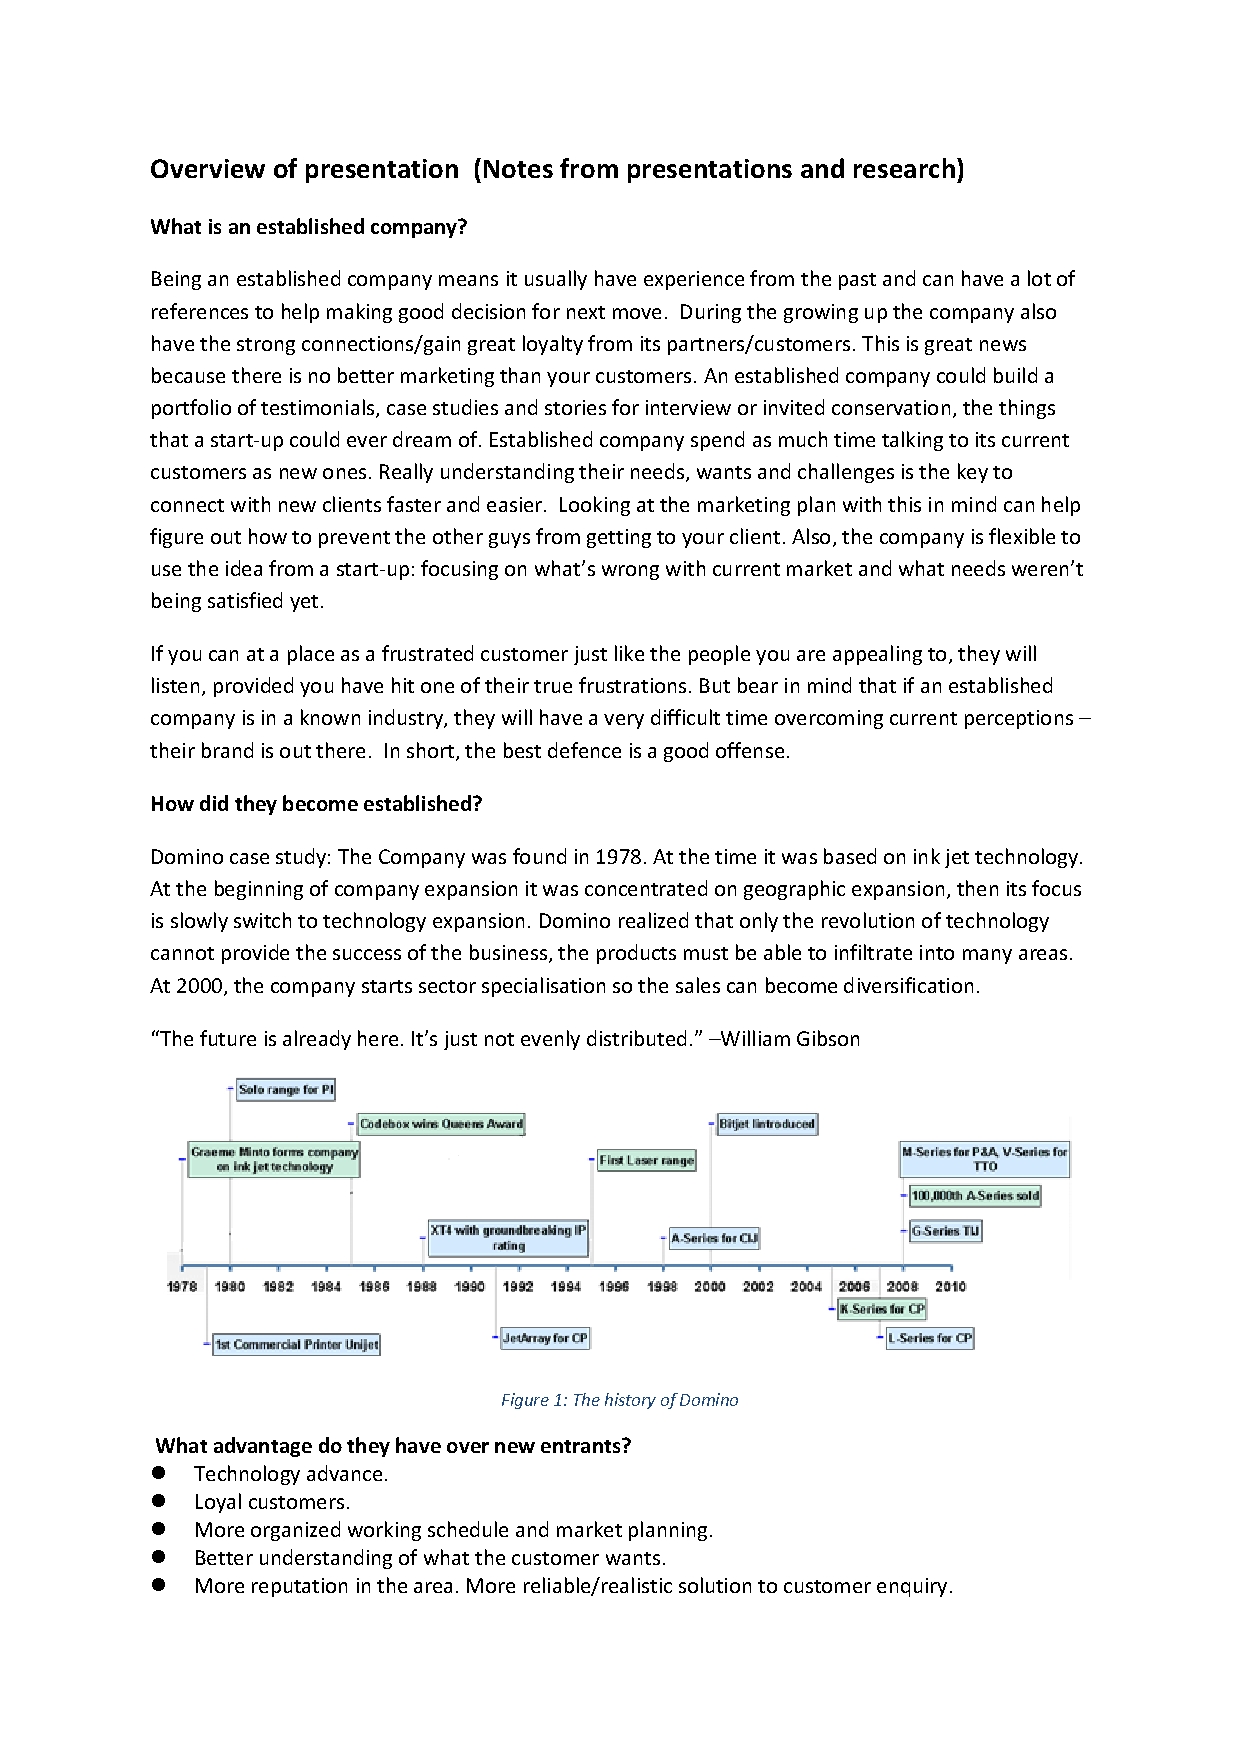
\includegraphics[width = 0.9\textwidth]{Figures/Overview_of_presentations}
		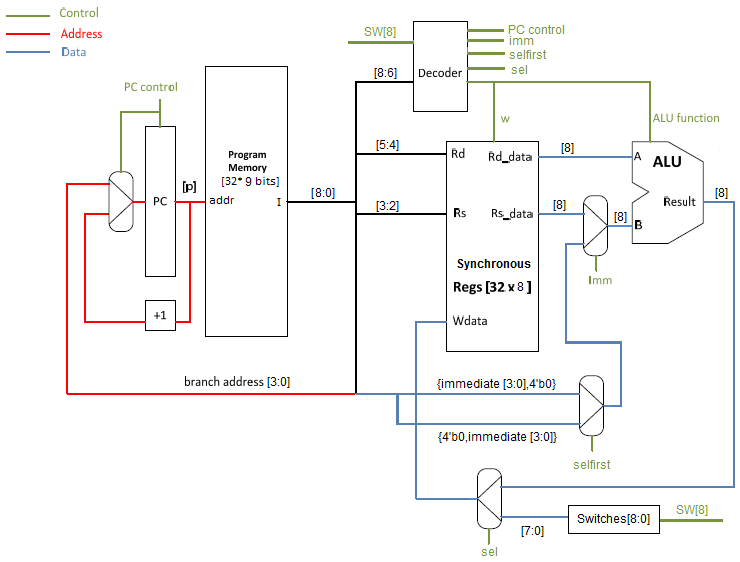
\includegraphics[width = \textwidth]{Figures/newarch}		
		\caption{The optimized picoMIPS architecture \cite{oldarcdigram}}
		\label {fig:newarc}
\end{figure}

\subsection{Improved design DE0 implementaion}
The simulation of new CPU is shown in Figure~\ref{fig:icputest}. The testbench is almost identical to the original one, expect it uses shorter instruction length.\\\\
The simulation results illustrates the same transform result as the original CPU. The immediate operand signal Alub shows that immediate value was correctly reformed despite the short immediate bits. The new behaviour of register was also well sorted by the new decoder as designed. The writing and read procedure were working properly during the affine transform from 450ns to 730ns. Because of the hexadecimal format, the instructions were extended to 12 bits with 0s to avoid the lenght truncation warning by the synthesis tool. 

\begin{figure}[H]
		\centering
		%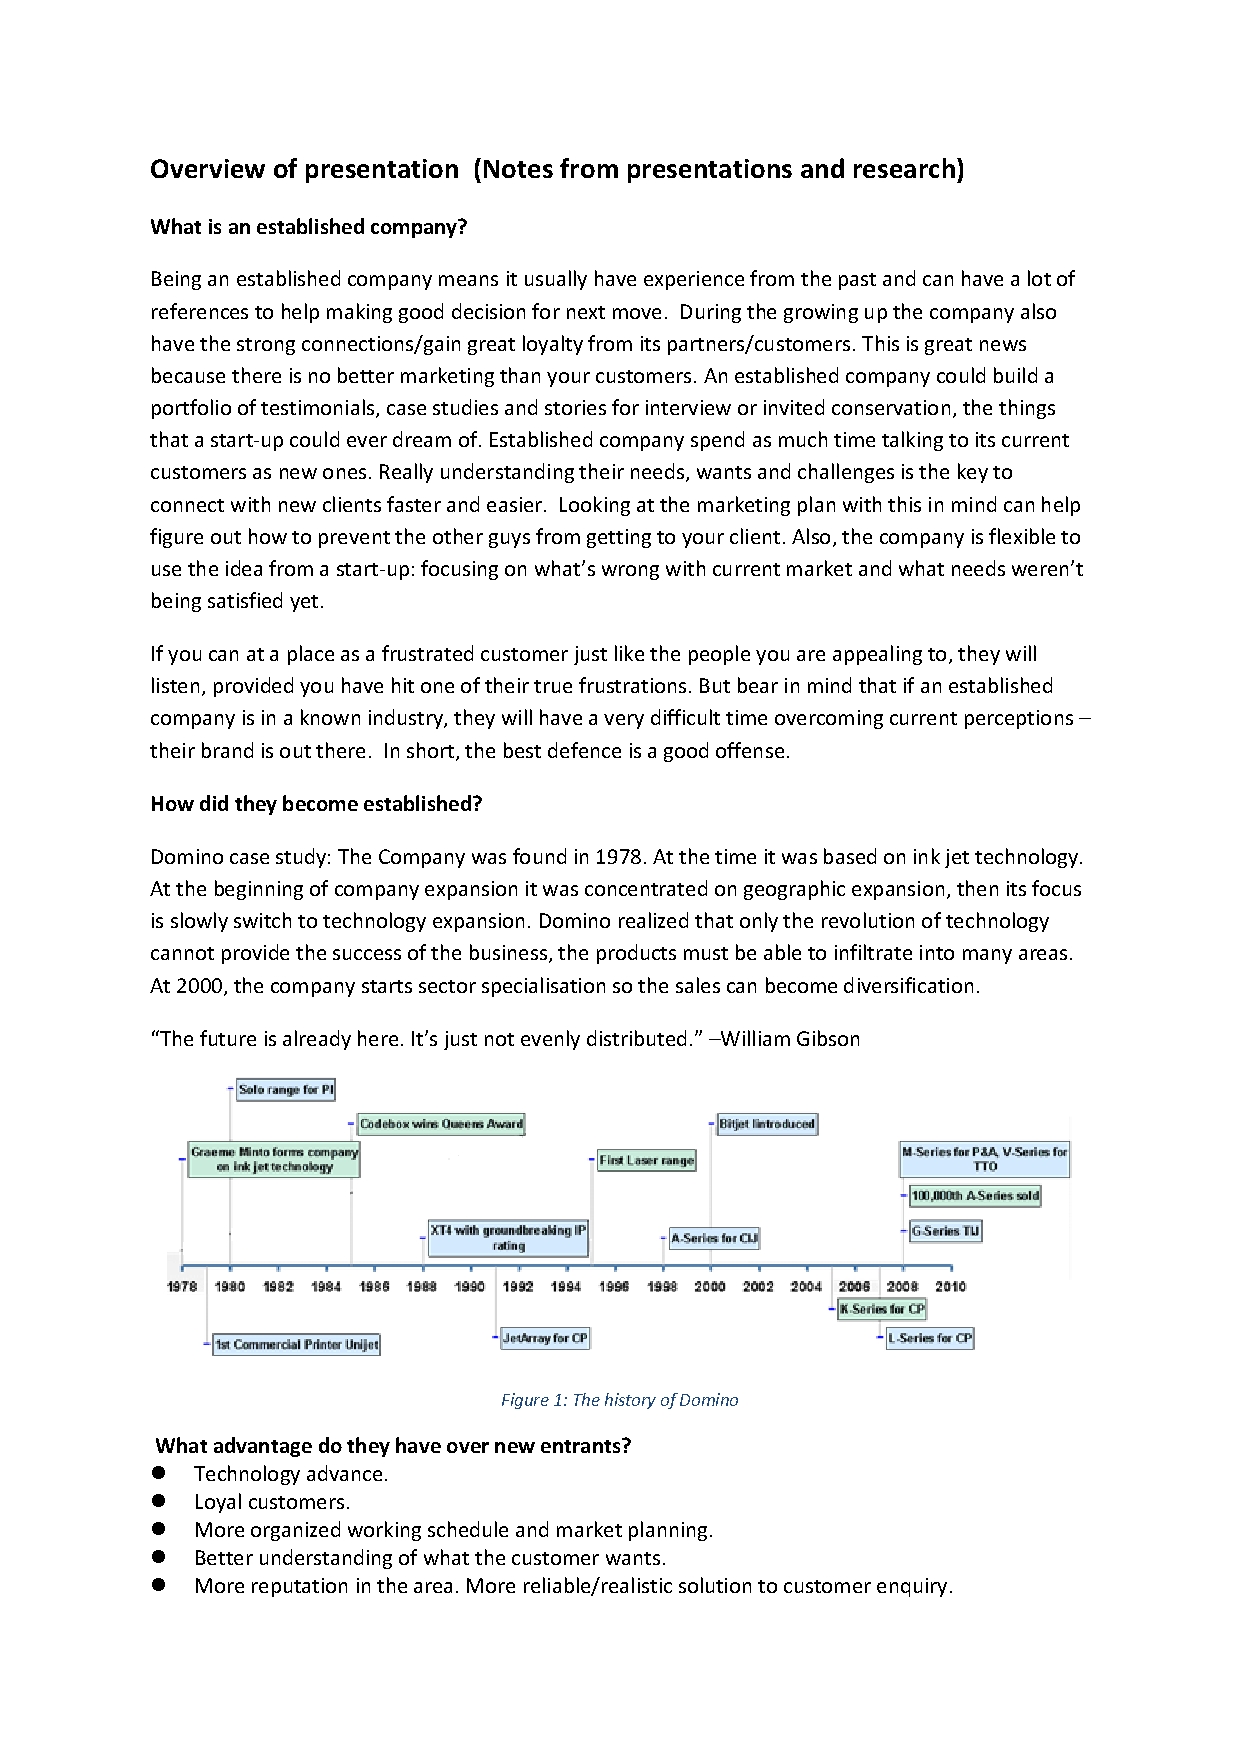
\includegraphics[width = 0.9\textwidth]{Figures/Overview_of_presentations}
		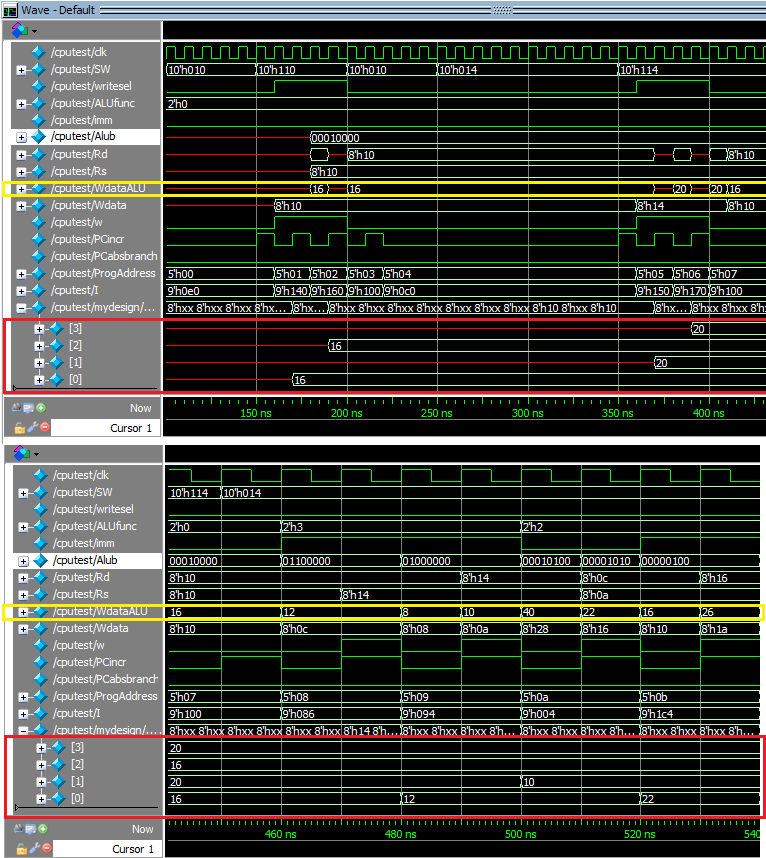
\includegraphics[width = \textwidth]{Figures/icputest_1}		
		%\caption{Simulation result of New CPU. (register values in the red box, output in the yellow box, immediate signal Alub is white highlighted)}
		%\label {fig:icputest}
\end{figure}

\begin{figure}[H]
		\centering
		%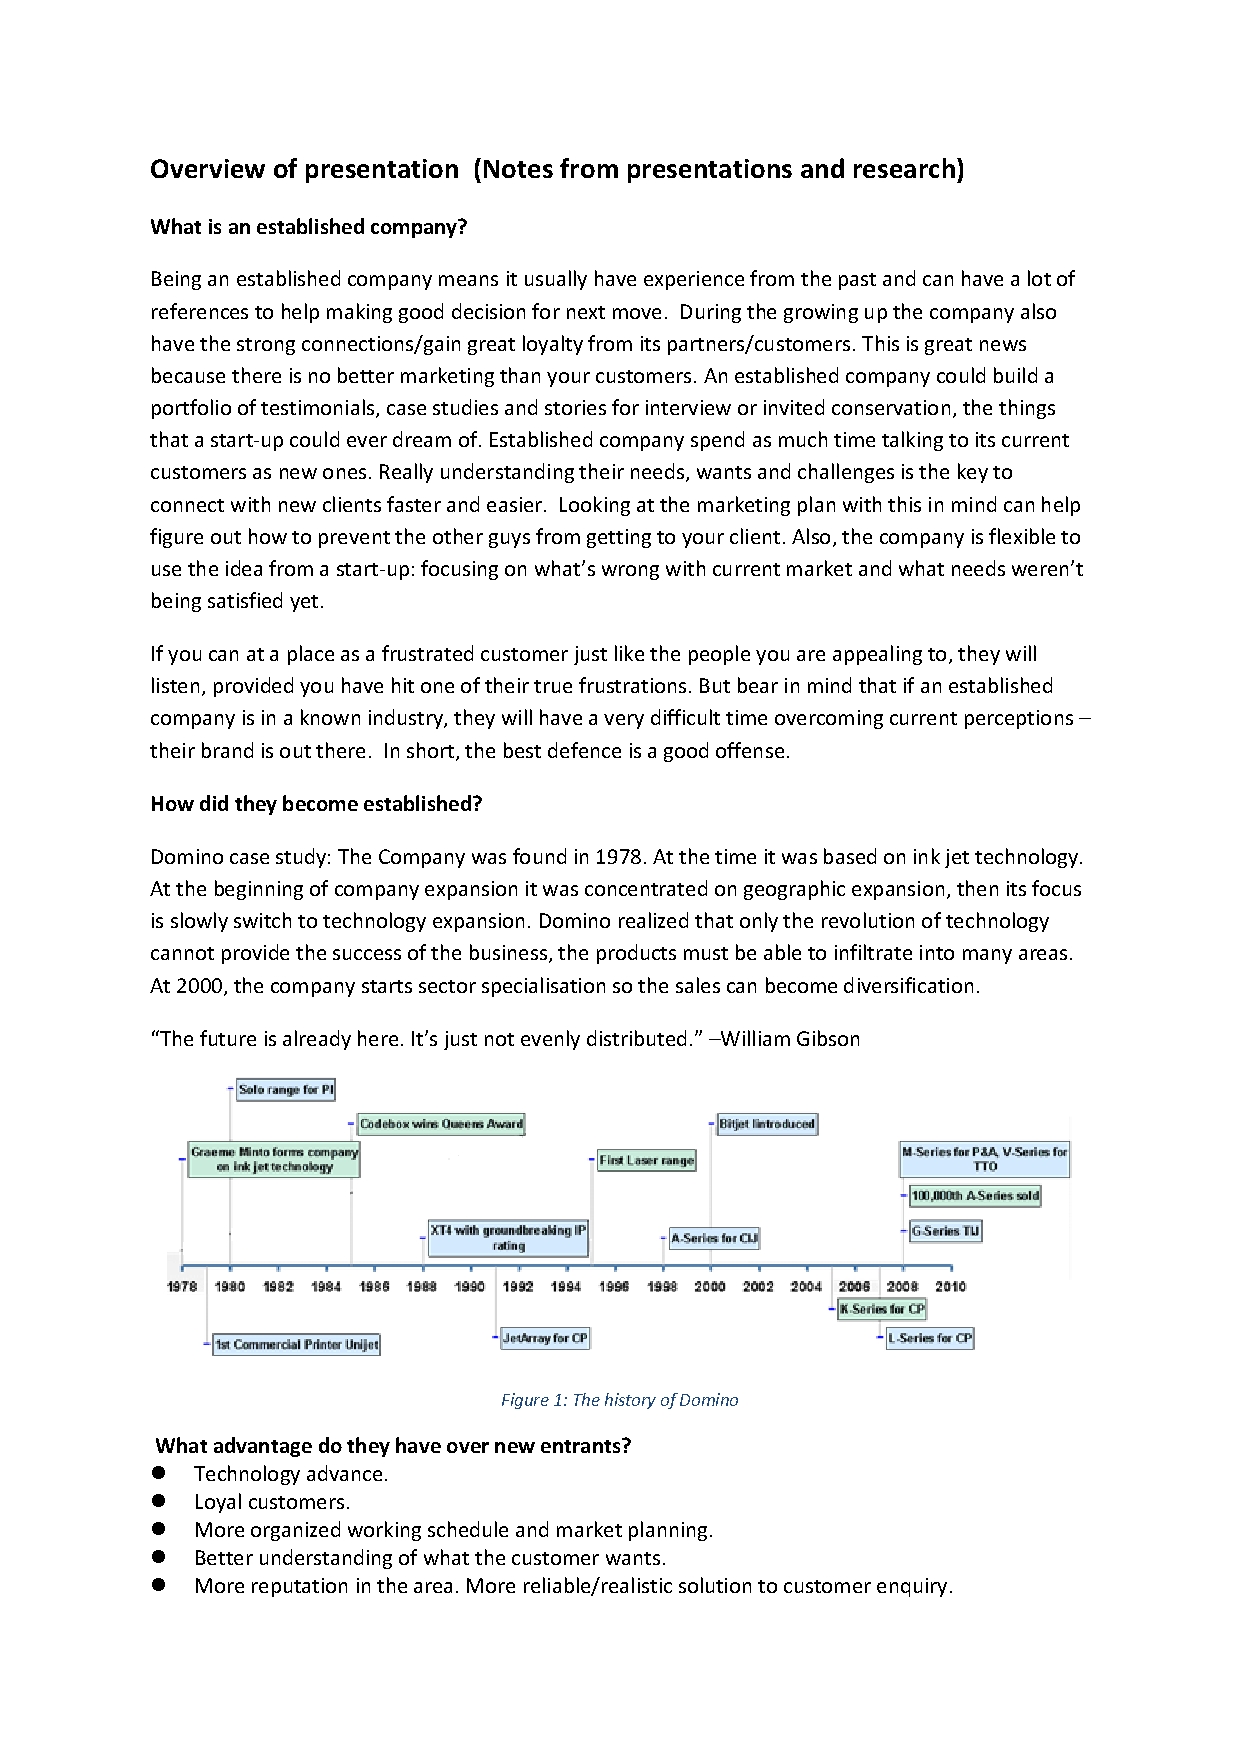
\includegraphics[width = 0.9\textwidth]{Figures/Overview_of_presentations}
		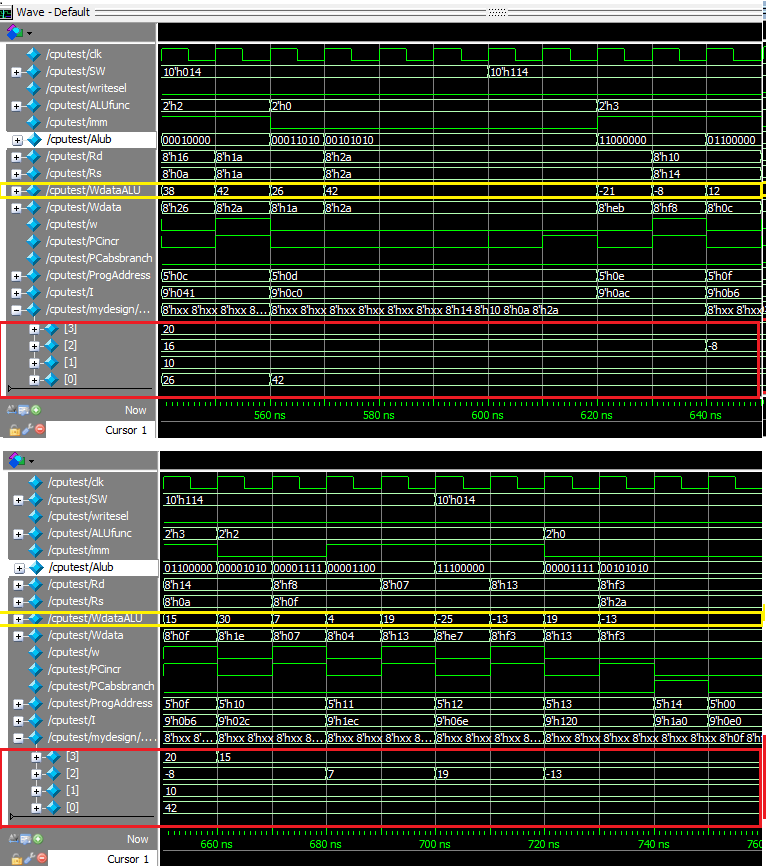
\includegraphics[width = \textwidth]{Figures/icputest_2}		
		\caption{Simulation result of New CPU. (register values in the red box, output in the yellow box, immediate signal Alub is highlighted in white box)}
		\label {fig:icputest}
\end{figure}

The improved picoMIPS processor generated the same results as the original one on the FPGA, by using the identical pixel coordinates, but the cost figure was significantly reduced (Figure~\ref{fig:icpugood}).

\begin{figure}[H]
		\centering
		%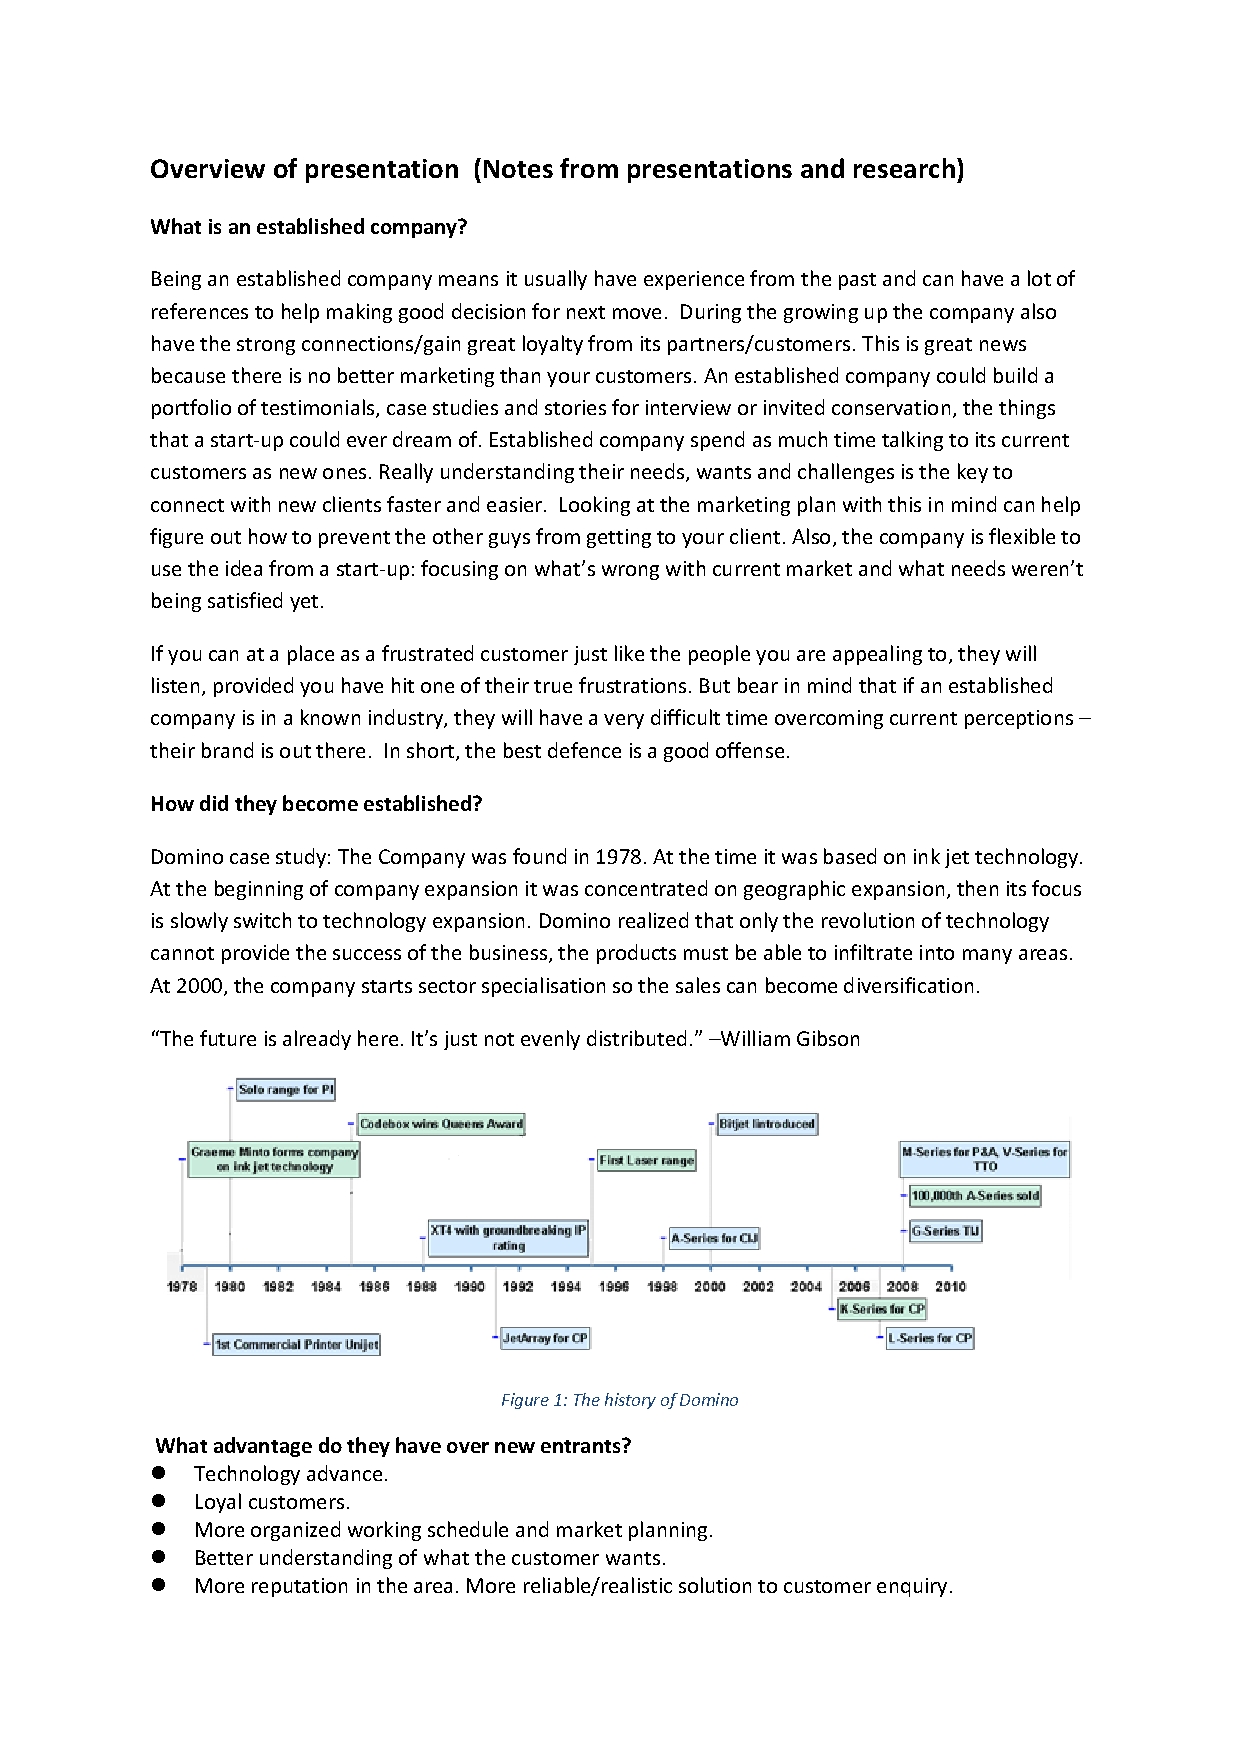
\includegraphics[width = 0.9\textwidth]{Figures/Overview_of_presentations}
		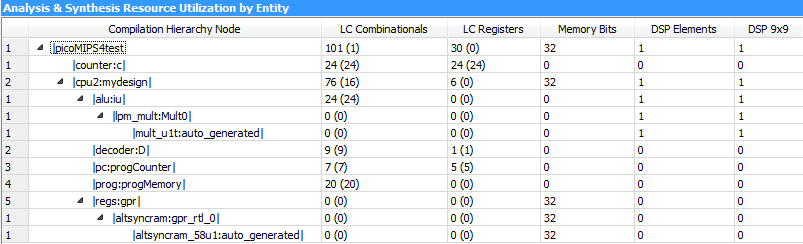
\includegraphics[width = \textwidth]{Figures/icpucost_1}		
		\caption{synthesis statistics of the improved CPU}
		\label {fig:icpugood}
\end{figure}
\chapter{Conclusions}




%\addcontentsline{toc}{chapter}{References}
\bibliographystyle{ieeetran}
\bibliography{Special/First_References}
%\end{document}
%% ----------------------------------------------------------------


%\appendix
%\appendixpage
%\addappheadtotoc
%%% ----------------------------------------------------------------
%% AppendixA.tex
%% ---------------------------------------------------------------- 


%\chapter{Something} \label{Chapter:Something}
\section{Statement of Contribution} \label{Section:Contribution}

Tables \ref{tab:jobs} and \ref{tab:jobs2} below detail the contributions of team members to the project.  While Ken Payne served as Team lead, Xuan Ban and Arinze Ekwosimba worked under his able leadership to ensure the project was delivered as required.  All members did significant research and contributed to the report writing as well.  The relative contribution of all authors is approximately equal.

\begin{table}
\begin{center}
\renewcommand{\arraystretch}{1.3}
\setlength{\tabcolsep}{7pt}
\begin{tabular}{ll}
\hline
\textbf{Group Member} & \textbf{Writing Task}\\
\hline
Arinze Ekwosimba & General editing of report, Wrote Abstract and Section Two (BT). \\
Kenneth Payne & Team Lead, wrote Introduction, Section One and Section Two (Intel) \\
Xuan Ban & Wrote Section Two (Nokia), Conclusion and Additional Notes \\
\hline
\end{tabular}
\caption{Report writing task allocation}
\label{tab:jobs}%
\end{center}
\end{table}

\begin{table}
\begin{center}
\renewcommand{\arraystretch}{1.3}
\setlength{\tabcolsep}{7pt}
\begin{tabular}{ll}
\hline
\textbf{Group Member} & \textbf{Research Task}\\
\hline
Arinze Ekwosimba & Gathered evidence on BT and Intel \\
Kenneth Payne & Gathered evidence on Intel \\
Xuan Ban & Gathered evidence on Nokia \\
\hline
\end{tabular}
\caption{Evidence Collation task allocation}
\label{tab:jobs2}%
\end{center}
\end{table}
%%% ----------------------------------------------------------------
%% AppendixB.tex
%% ---------------------------------------------------------------- 


%\chapter{Something} \label{Chapter:Something}
\section{Meeting Minutes} \label{Section:Minutes}

	\begin{figure}[ht!]
		\centering
		\includegraphics[width = 0.9\textwidth]{Figures/Minutes_1}
		\caption[Minutes I]{Minutes of the first group meeting}
		\label {fig:minutes:one}
	\end{figure}
	
		\begin{figure}[ht!]
		\centering
		\includegraphics[width = 0.9\textwidth]{Figures/Minutes_2}
		\caption[Minutes II]{Minutes of the second group meeting}
		\label {fig:minutes:two}
	\end{figure}
	
		\begin{figure}[ht!]
		\centering
		\includegraphics[width = 0.9\textwidth]{Figures/Minutes_3}
		\caption[Minutes III]{Minutes of the third group meeting}
		\label {fig:minutes:three}
	\end{figure}
%%% ----------------------------------------------------------------
%% AppendixC.tex
%% ---------------------------------------------------------------- 


%\chapter{Something} \label{Chapter:Something}
\section{Additional Notes} \label{Section:Notes}


	\begin{figure}[ht!]
		\centering
		%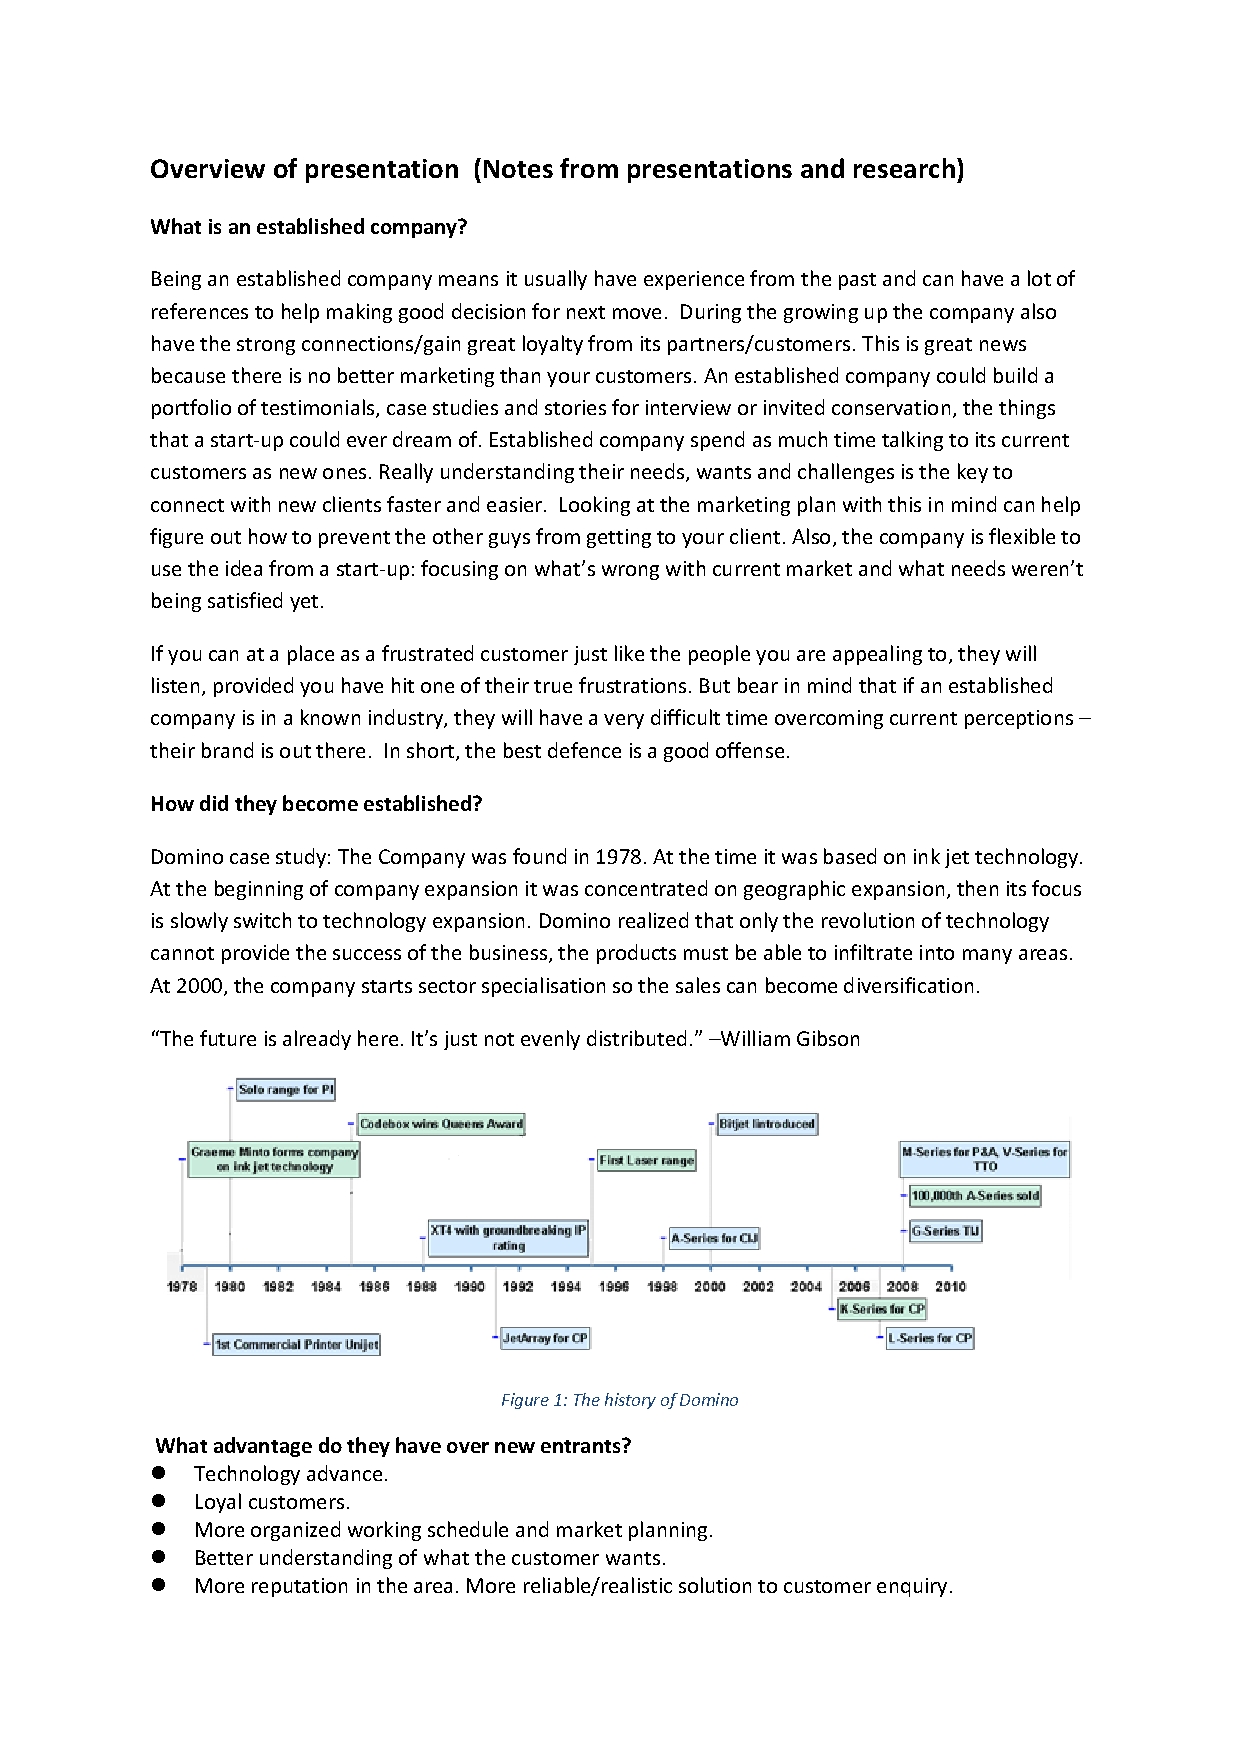
\includegraphics[width = 0.9\textwidth]{Figures/Overview_of_presentations}
		\includegraphics[width = 0.9\textwidth, page=1]{Figures/Overview_of_presentations}		
		%\caption[Additional Notes]{Notes taken for given presentations and independent research}
		\label {fig:additional:notes1}
	\end{figure}
	
		\begin{figure}[ht!]
		\centering
		%\includegraphics[width = 0.9\textwidth]{Figures/Overview_of_presentations}
		\includegraphics[width = \textwidth, page=2]{Figures/Overview_of_presentations}		
		%\caption[Additional Notes]{Notes taken for given presentations and independent research}
		\label {fig:additional:notes2}
	\end{figure}
	
		\begin{figure}[ht!]
		\centering
		%\includegraphics[width = 0.9\textwidth]{Figures/Overview_of_presentations}
		\includegraphics[width = \textwidth, page=3]{Figures/Overview_of_presentations}		
		%\caption[Additional Notes]{Notes taken for given presentations and independent research}
		\label {fig:additional:notes3}
	\end{figure}
	
		\begin{figure}[ht!]
		\centering
		%\includegraphics[width = 0.9\textwidth]{Figures/Overview_of_presentations}
		\includegraphics[width = \textwidth, page=4]{Figures/Overview_of_presentations}		
		%\caption[Additional Notes]{Notes taken for given presentations and independent research}
		\label {fig:additional:notes4}
	\end{figure}
	
		\begin{figure}[ht!]
		\centering
		%\includegraphics[width = 0.9\textwidth]{Figures/Overview_of_presentations}
		\includegraphics[width = \textwidth, page=5]{Figures/Overview_of_presentations}		
		\caption[Additional Notes]{Notes taken for given presentations and independent research}
		\label {fig:additional:notes5}
	\end{figure}
%\include{Appendices/AppendixD}
%\include{Appendices/AppendixE}

\end{document}